
\documentclass[xcolor=table]{beamer}
\usepackage[spanish,es-tabla]{babel}
\usepackage[utf8x]{inputenc}
\usepackage{adjustbox}
\usepackage[labelformat=empty]{caption}
\usepackage[justification=centering]{caption}

\mode<presentation> {

\usetheme{Boadilla}



\setbeamertemplate{footline}[page number] % To replace the footer line in all slides with a simple slide count uncomment this line

\setbeamertemplate{navigation symbols}{} % To remove the navigation symbols from the bottom of all slides uncomment this line 
}

\usepackage{amsmath} 
\usepackage{graphicx} % Allows including images
\usepackage{booktabs} % Allows the use of \toprule, \midrule and \bottomrule in tables
\usepackage[table]{xcolor}

%\usepackage[style=ieee]{biblatex} %Use if necessary for citation
%\addbibresource{biblatex-examples.bib}


%----------------------------------------------------------------------------------------
%	TITLE PAGE
%----------------------------------------------------------------------------------------

\title{Probabilistic shaping\\ \small Practica Profesional Supervisada} % The short title appears at the bottom of every slide, the full title is only on the title page

\author{\small Dipre Ivan\\ \small Viglianco Kevin H.\\ \vspace{0.2cm} \small Supervisior: Dr. Ariel L. Pola} % Your name

\date{\today} % Date, can be changed to a custom date

\begin{document}

\begin{frame}
\titlepage % Print the title page as the first slide
\begin{figure}[H]
\centering

\includegraphics[width=45mm]{fulgor_logo1.png}
\end{figure}

\end{frame}

\begin{frame}
\frametitle{\'Indice} 
\tableofcontents 
\end{frame}

\section{Introducci\'on}
\begin{frame}{Introducción}
    \begin{itemize}
        \item La técnica `probabilistic shaping' permite modificar la probabilidad de ocurrencia de cada símbolo en una transmisión digital, modificando la forma de su constelación.

        \item Para esto se utiliza el método `distribution matching' el cual permite transformar una secuencia de entrada, con distribución uniforme, a una secuencia de salida con una distribución diferente. 
    \end{itemize}
\end{frame}

% \begin{frame}{Introducción}
% Esto es necesario porque permitirá:
%     \begin{itemize}
%         \item Reducir la potencia de transmisión 
%         \item Disminuir la tasa de error total
%     \end{itemize}
% \end{frame}

\section{Desarrollo}

\begin{frame}{Flujo de trabajo}

\begin{figure}[H]
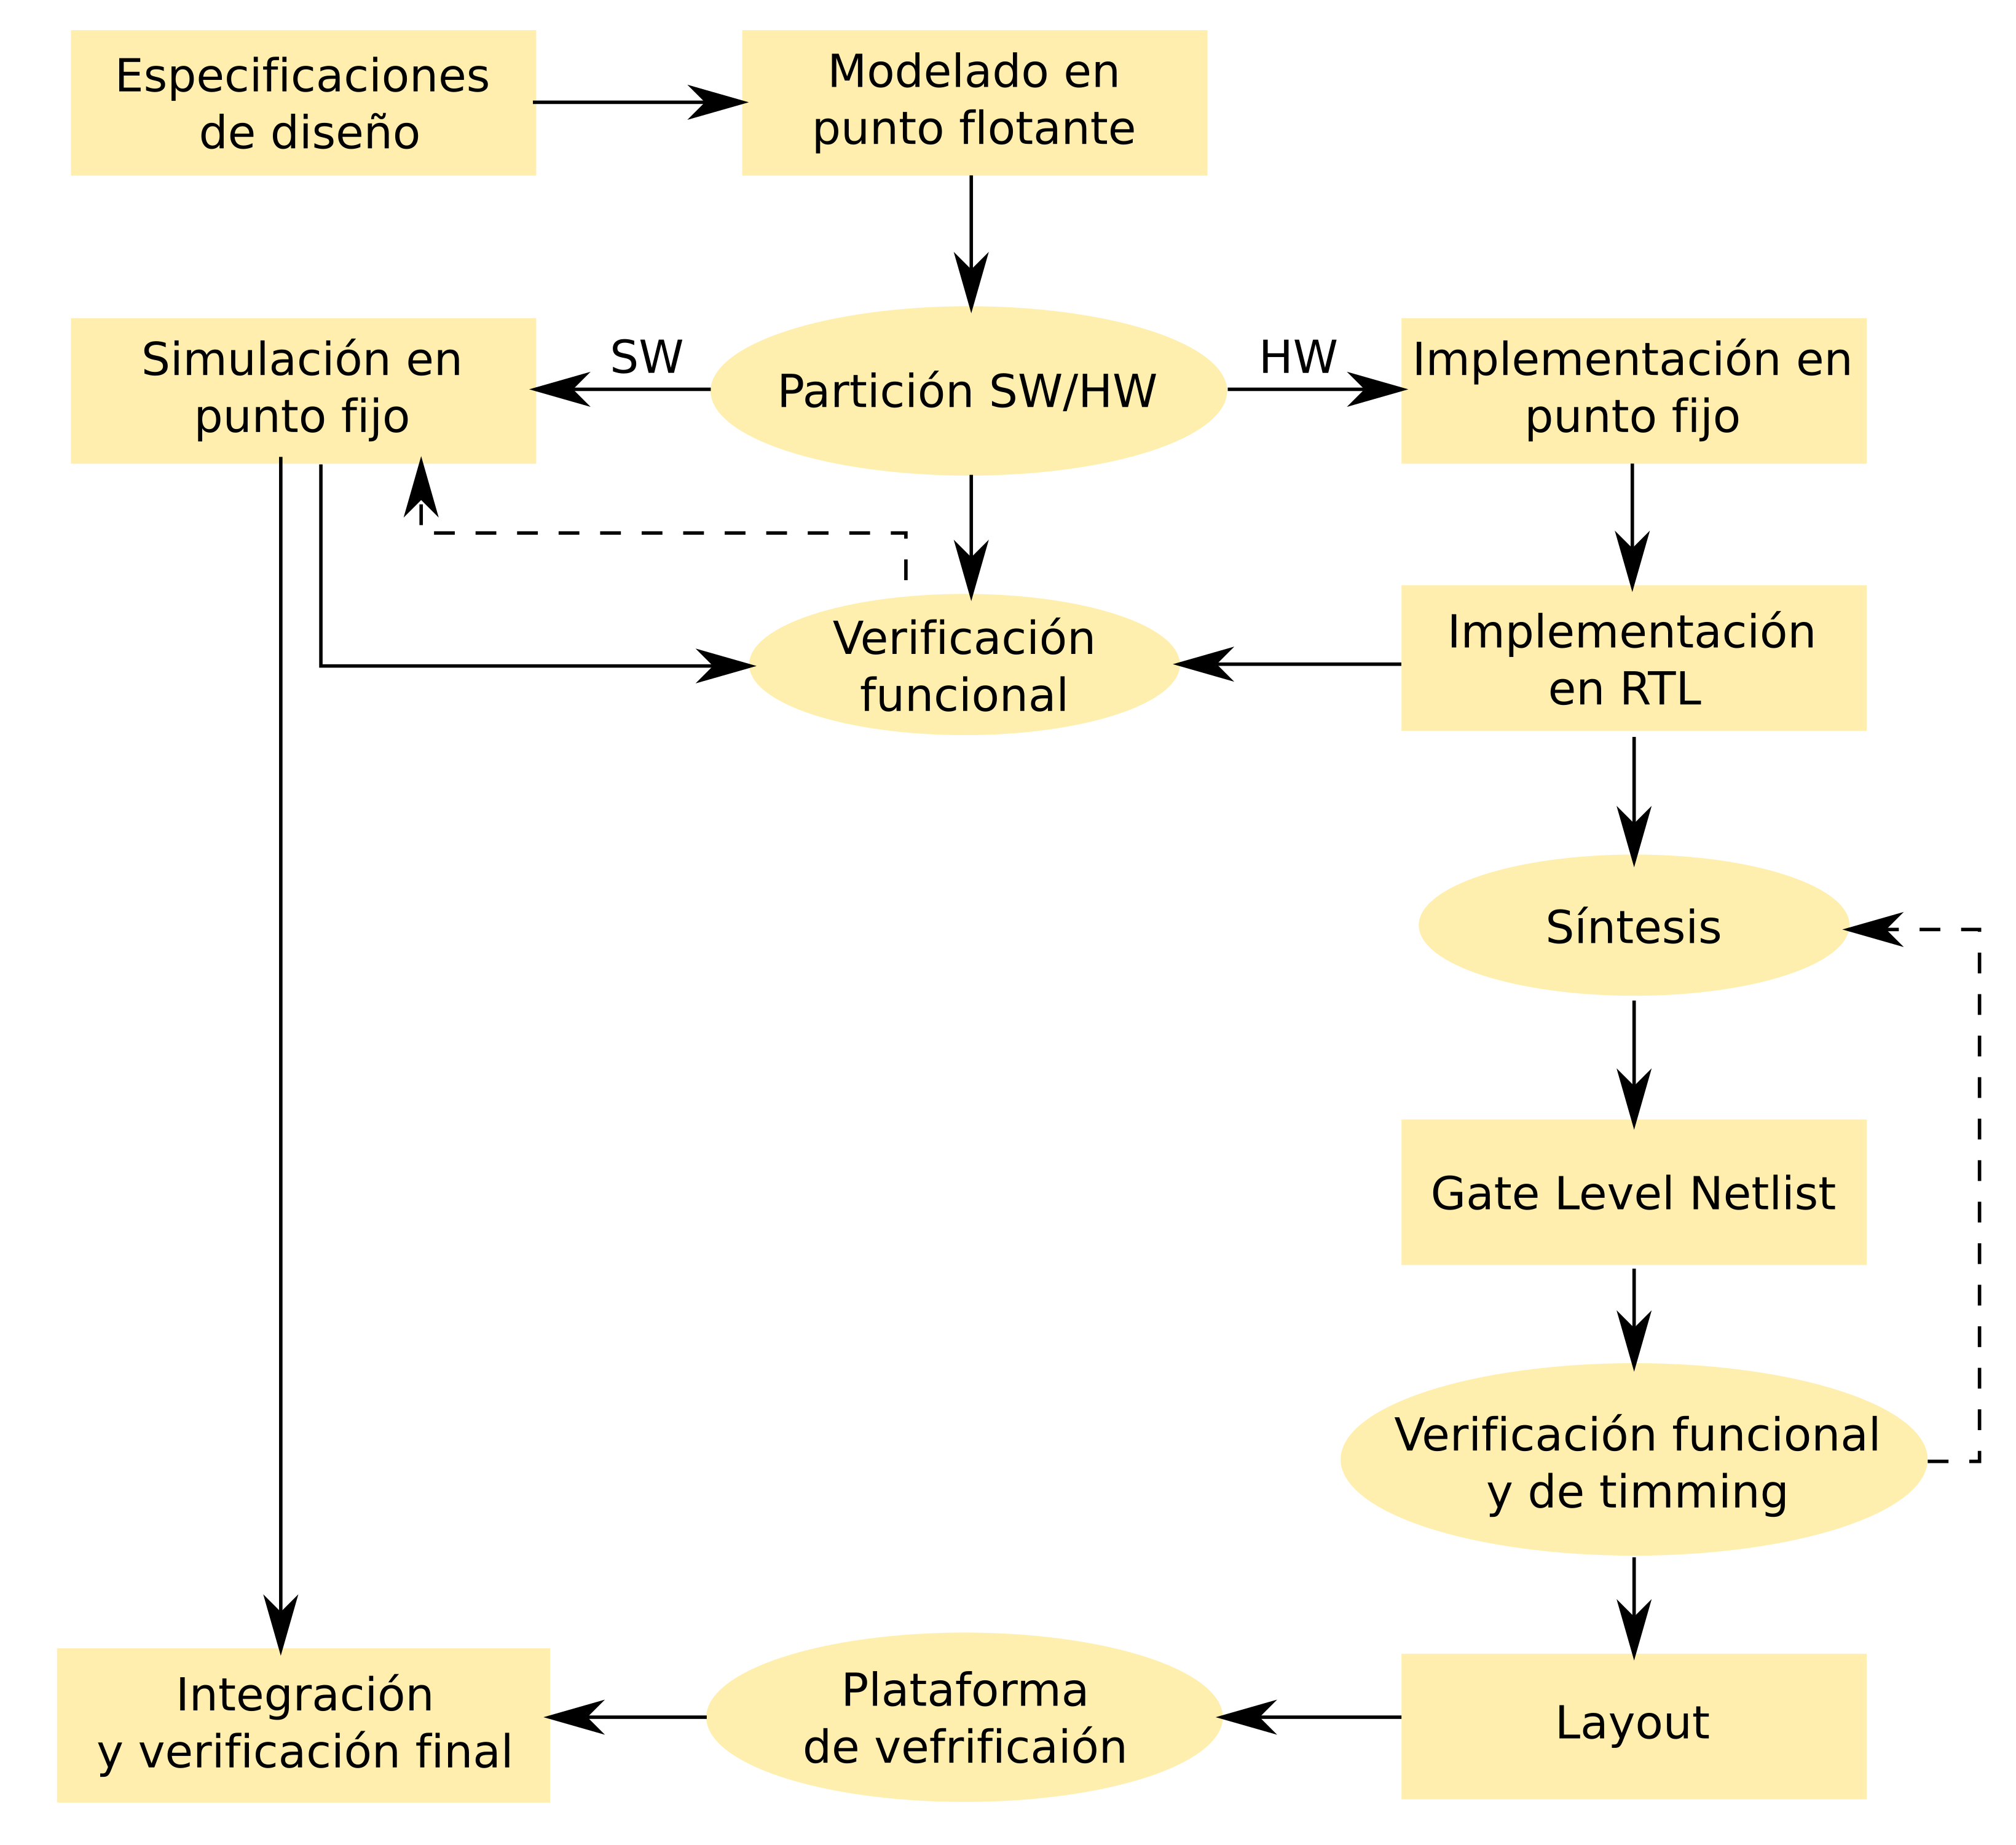
\includegraphics[width=0.65\paperwidth]{Diagramas/diag_flujo.png}
\end{figure}
\end{frame}

\subsection{Investigación y diseño}

\begin{frame}{Método `distribution matching' }
\begin{itemize}
    \item Transforma una salida DMS\footnote{Siglas en ingles de Generador Discreto Sin Memoria} en una secuencia que emula un DMS objetivo \cite{baur}.
\end{itemize}
\begin{figure}[H]
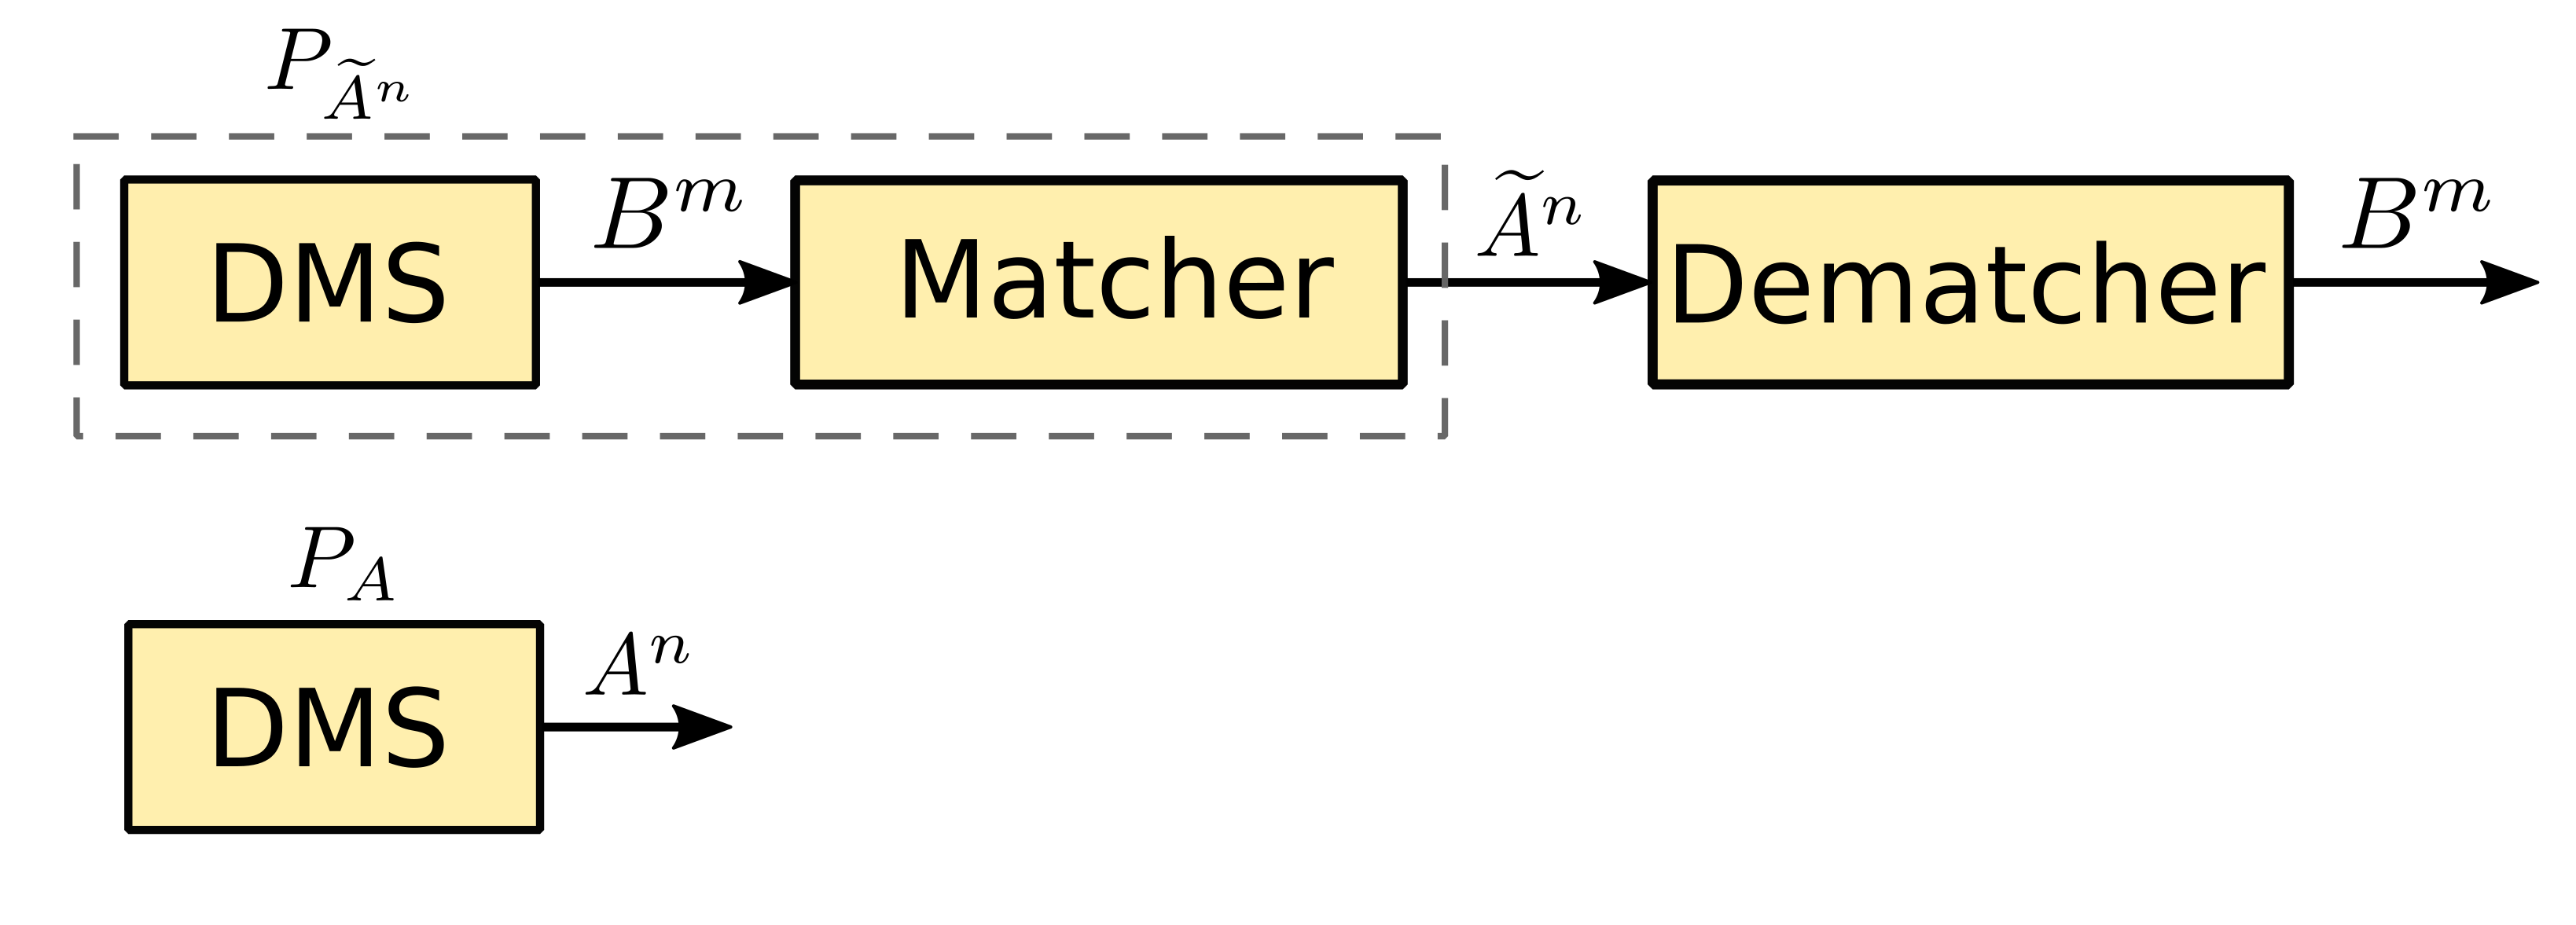
\includegraphics[width=0.70\paperwidth]{Diagramas/matcher.png}
\end{figure}
\end{frame}

\begin{frame}{Tipos de algoritmos}
\begin{itemize}
    \item Según la longitud de la secuencia de datos:
     \begin{itemize}
         \item Longitud variable a longitud variable (v2v).
        \item Longitud variable a longitud fija, o viceversa (v2f o f2v).
        \item Longitud fija a longitud fija (f2f).
     \end{itemize}
    \item Según modo de calculo
    \begin{itemize}
        \item Online, es decir, en tiempo real
        \item Offline, es decir, de forma precalculada
    \end{itemize}
\end{itemize}
\end{frame}



\begin{frame}{Especificaciones de diseño}
\begin{itemize}
    \item A partir de un DMS con distribución $ P_{(x=0)}= P_{(x=1)}=0.5$ obtener una distribución con una probabilidad de ceros de $P_{(x=0)}= 0.75$.
    \item La secuencia de entrada al codificador deberá ser de 4 bits.
    \item Implementar el mismo con una modulación QAM-16.
\end{itemize}
\end{frame}


\begin{frame}{Selección del algoritmo a utilizar}
\begin{itemize}
    \item Se utilizará el algoritmo `Constant Composition Distribution Matching' propuesto en \cite{schulte}
    \item El mismo trabaja con longitudes fijas (f2f) y el calculo es de tipo `online' 
    % \item Es una técnica de complejidad relativamente baja
\end{itemize}
\end{frame}


\begin{frame}{Desarrollo del algoritmo ‘Constant Composition’ }
\begin{enumerate}
    \item Utiliza 'arithmetic coding'.
    \item Asocia un intervalo a cada una de las posibles entradas y salidas en base a su probabilidad
    \item Realiza un mapeo de cada intervalo de entrada a un unico intervalo de salida
    \item Todas las secuencias de salida tienen una composición constante de `0' y `1'.
    % Insertar imagen intervalos
\end{enumerate}
\end{frame}

\begin{frame}{Longitud de palabra de salida}
\begin{itemize}
\item Esta depende de: 
\begin{itemize}
    \item  Cantidad de bits de entrada
    \item La probabilidad $P_{(x=1)}$ deseada
\end{itemize}
    \item Se debe cumplir que:
        \begin{equation*}
        XCY \geq 2^{k}    
        \end{equation*}
    \item Donde:
        \begin{itemize}
            \item [$C$:]  Combinatoria
            \item [$Y$:]  Cantidad de bits de salida en `1'
            \item [$X$:] Longitud de salida
            \item[$k$:]  Longitud de secuencia entrada 
        \end{itemize}
    \item Además se debe mantener la relación:
        \begin{equation*}
        \frac{X}{Y} =  \frac{1}{P_{(x=1)}}  
        \end{equation*}
    
    
    \end{itemize}
\end{frame}

\begin{frame}{Longitud de palabra de salida}
    \begin{itemize}
        \item Para nuestro caso: $k=4$ y $P_{(x=1)} = 0.25$. Por lo tanto:
            \begin{equation*}
            \frac{X}{Y} = \frac{1}{P_{(x=1)}} = 4 \implies X = 4*Y
            \end{equation*}
        \item A su vez:
            \begin{equation*} 
            XCY \geq 16 \implies X=8 \implies \frac{X-k}{k} = 100\% 
            \end{equation*}
        \item Supongamos $k=16$ y $P_{(x=1)} = 0.25$. Tendremos
            \begin{equation*} 
            24C6 \geq 2^{16} \implies X=24 \implies \frac{X-k}{k} = 50\% 
            \end{equation*}
        \item Por otro lado, si $k=4$ y $P_{(x=1)} = 0.285$. Tendremos:
            \begin{equation*} 
            7C2 \geq 2^{4} \implies X=7 \implies \frac{X-k}{k} = 75\% 
            \end{equation*}
    \end{itemize}
\end{frame}


%\begin{frame}{Calculo de intervalo de entrada de bloque codificador}
%\begin{enumerate}
%    \item Se inicializan los limites superior e inferior: $u_i=1.0$ y $l_i=0.0$
%    \item Se selecciona un subintervalo en base al bit de entrada
%    \begin{itemize}
%        \item Si  $Xi_{cod}=1 \implies [0,5;1,0)$ 
%        \item Si  $Xi_{cod}=0 \implies (0,0;0,5]$ 
%    \end{itemize}
%    \item Se repiten los pasos anteriores tantas veces como bits de entrada se tengan
%    \item Se toma como salida el valor inferior del subintervalo final $l_i$
%\end{enumerate}
%\end{frame}
\begin{frame}{Calculo de intervalo de entrada de bloque codificador}

\begin{figure}
  \centering
  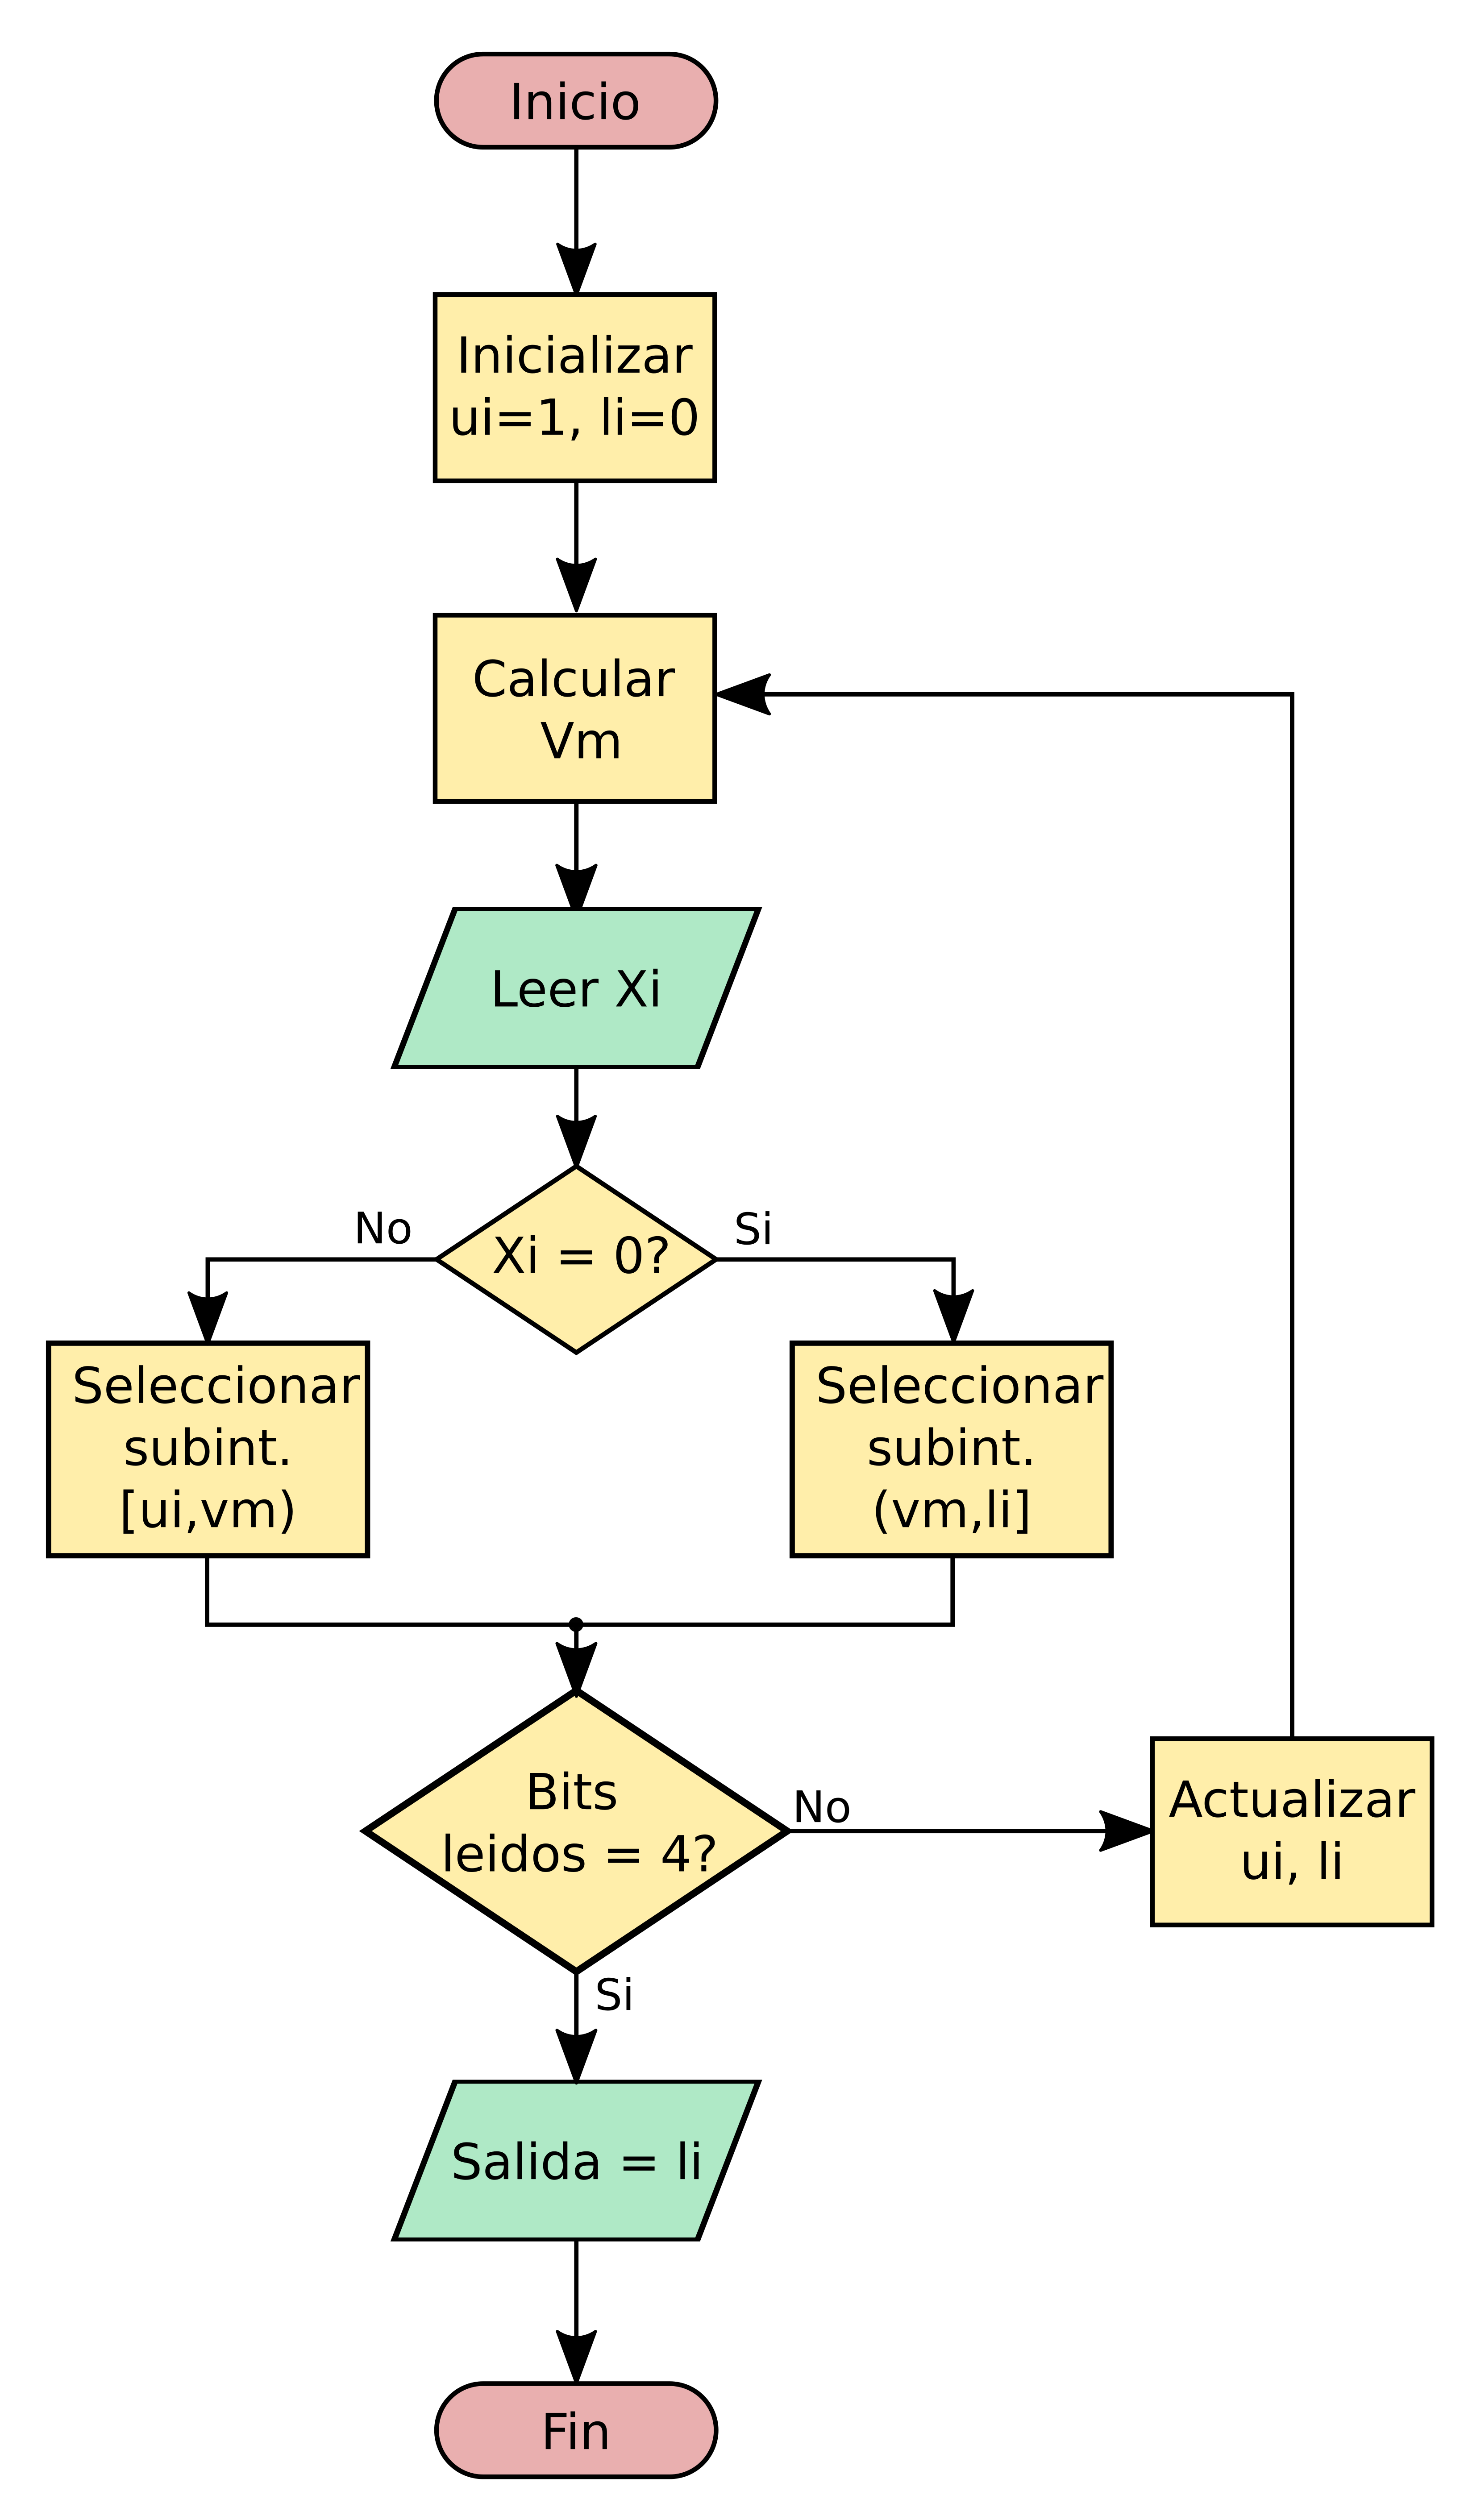
\includegraphics[ height=0.85\textheight]{Diagramas/diag_ciec.png}%
   \end{figure}

\end{frame}

\begin{frame}{Ejemplo de calculo de intervalo de entrada del bloque codificador}
\begin{itemize}
    \item Para $Xi_{cod} = 1010$ y $P_{(x=0)}=0.75$: 
\end{itemize}
\begin{figure}[H]
  \centering
  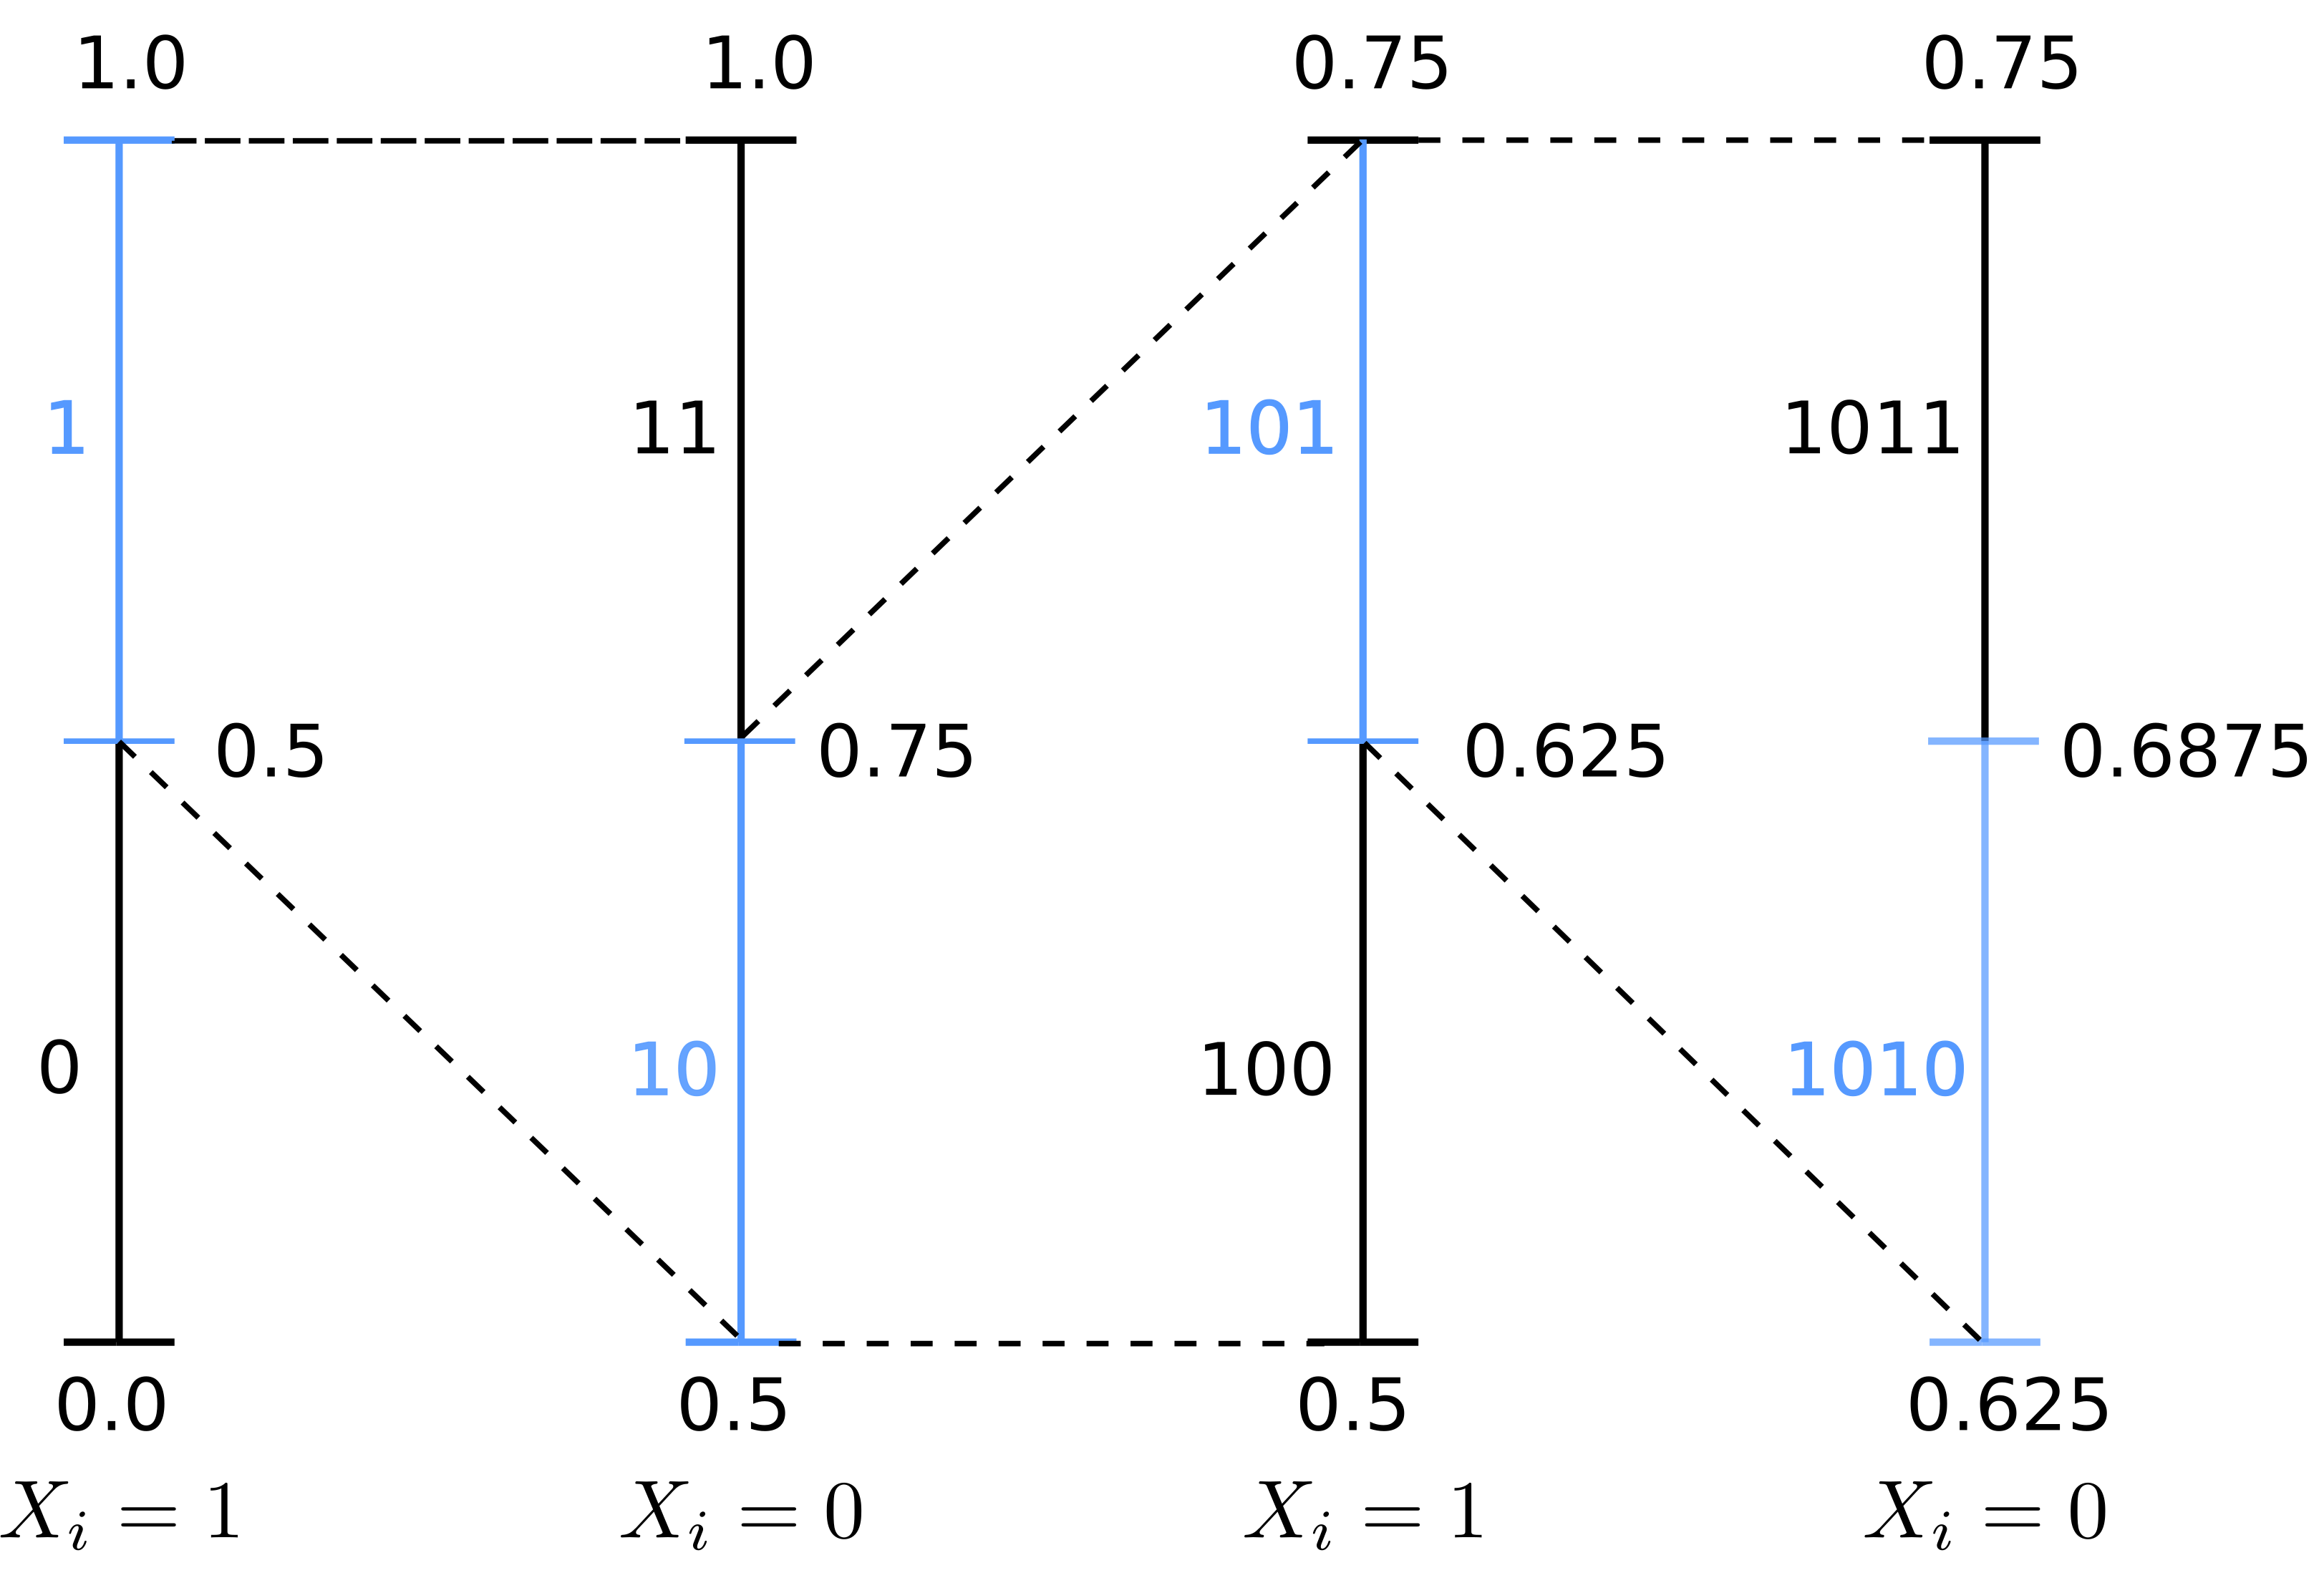
\includegraphics[width=0.80\paperheight]{Diagramas/int_ent_cod.png}%
   \end{figure}
\end{frame}

\begin{frame}{Calculo de intervalo de salida de bloque codificador}
\begin{itemize}
    \item Se utiliza el concepto de 'bolsa de bits' propuesto en \cite[Sec.\ 4]{schulte}
    \item En cada iteración se elimina un bit, obteniendo una nueva probabilidad $P_{(x=0)}$ 
\end{itemize}
\begin{figure}[H]
  \centering
  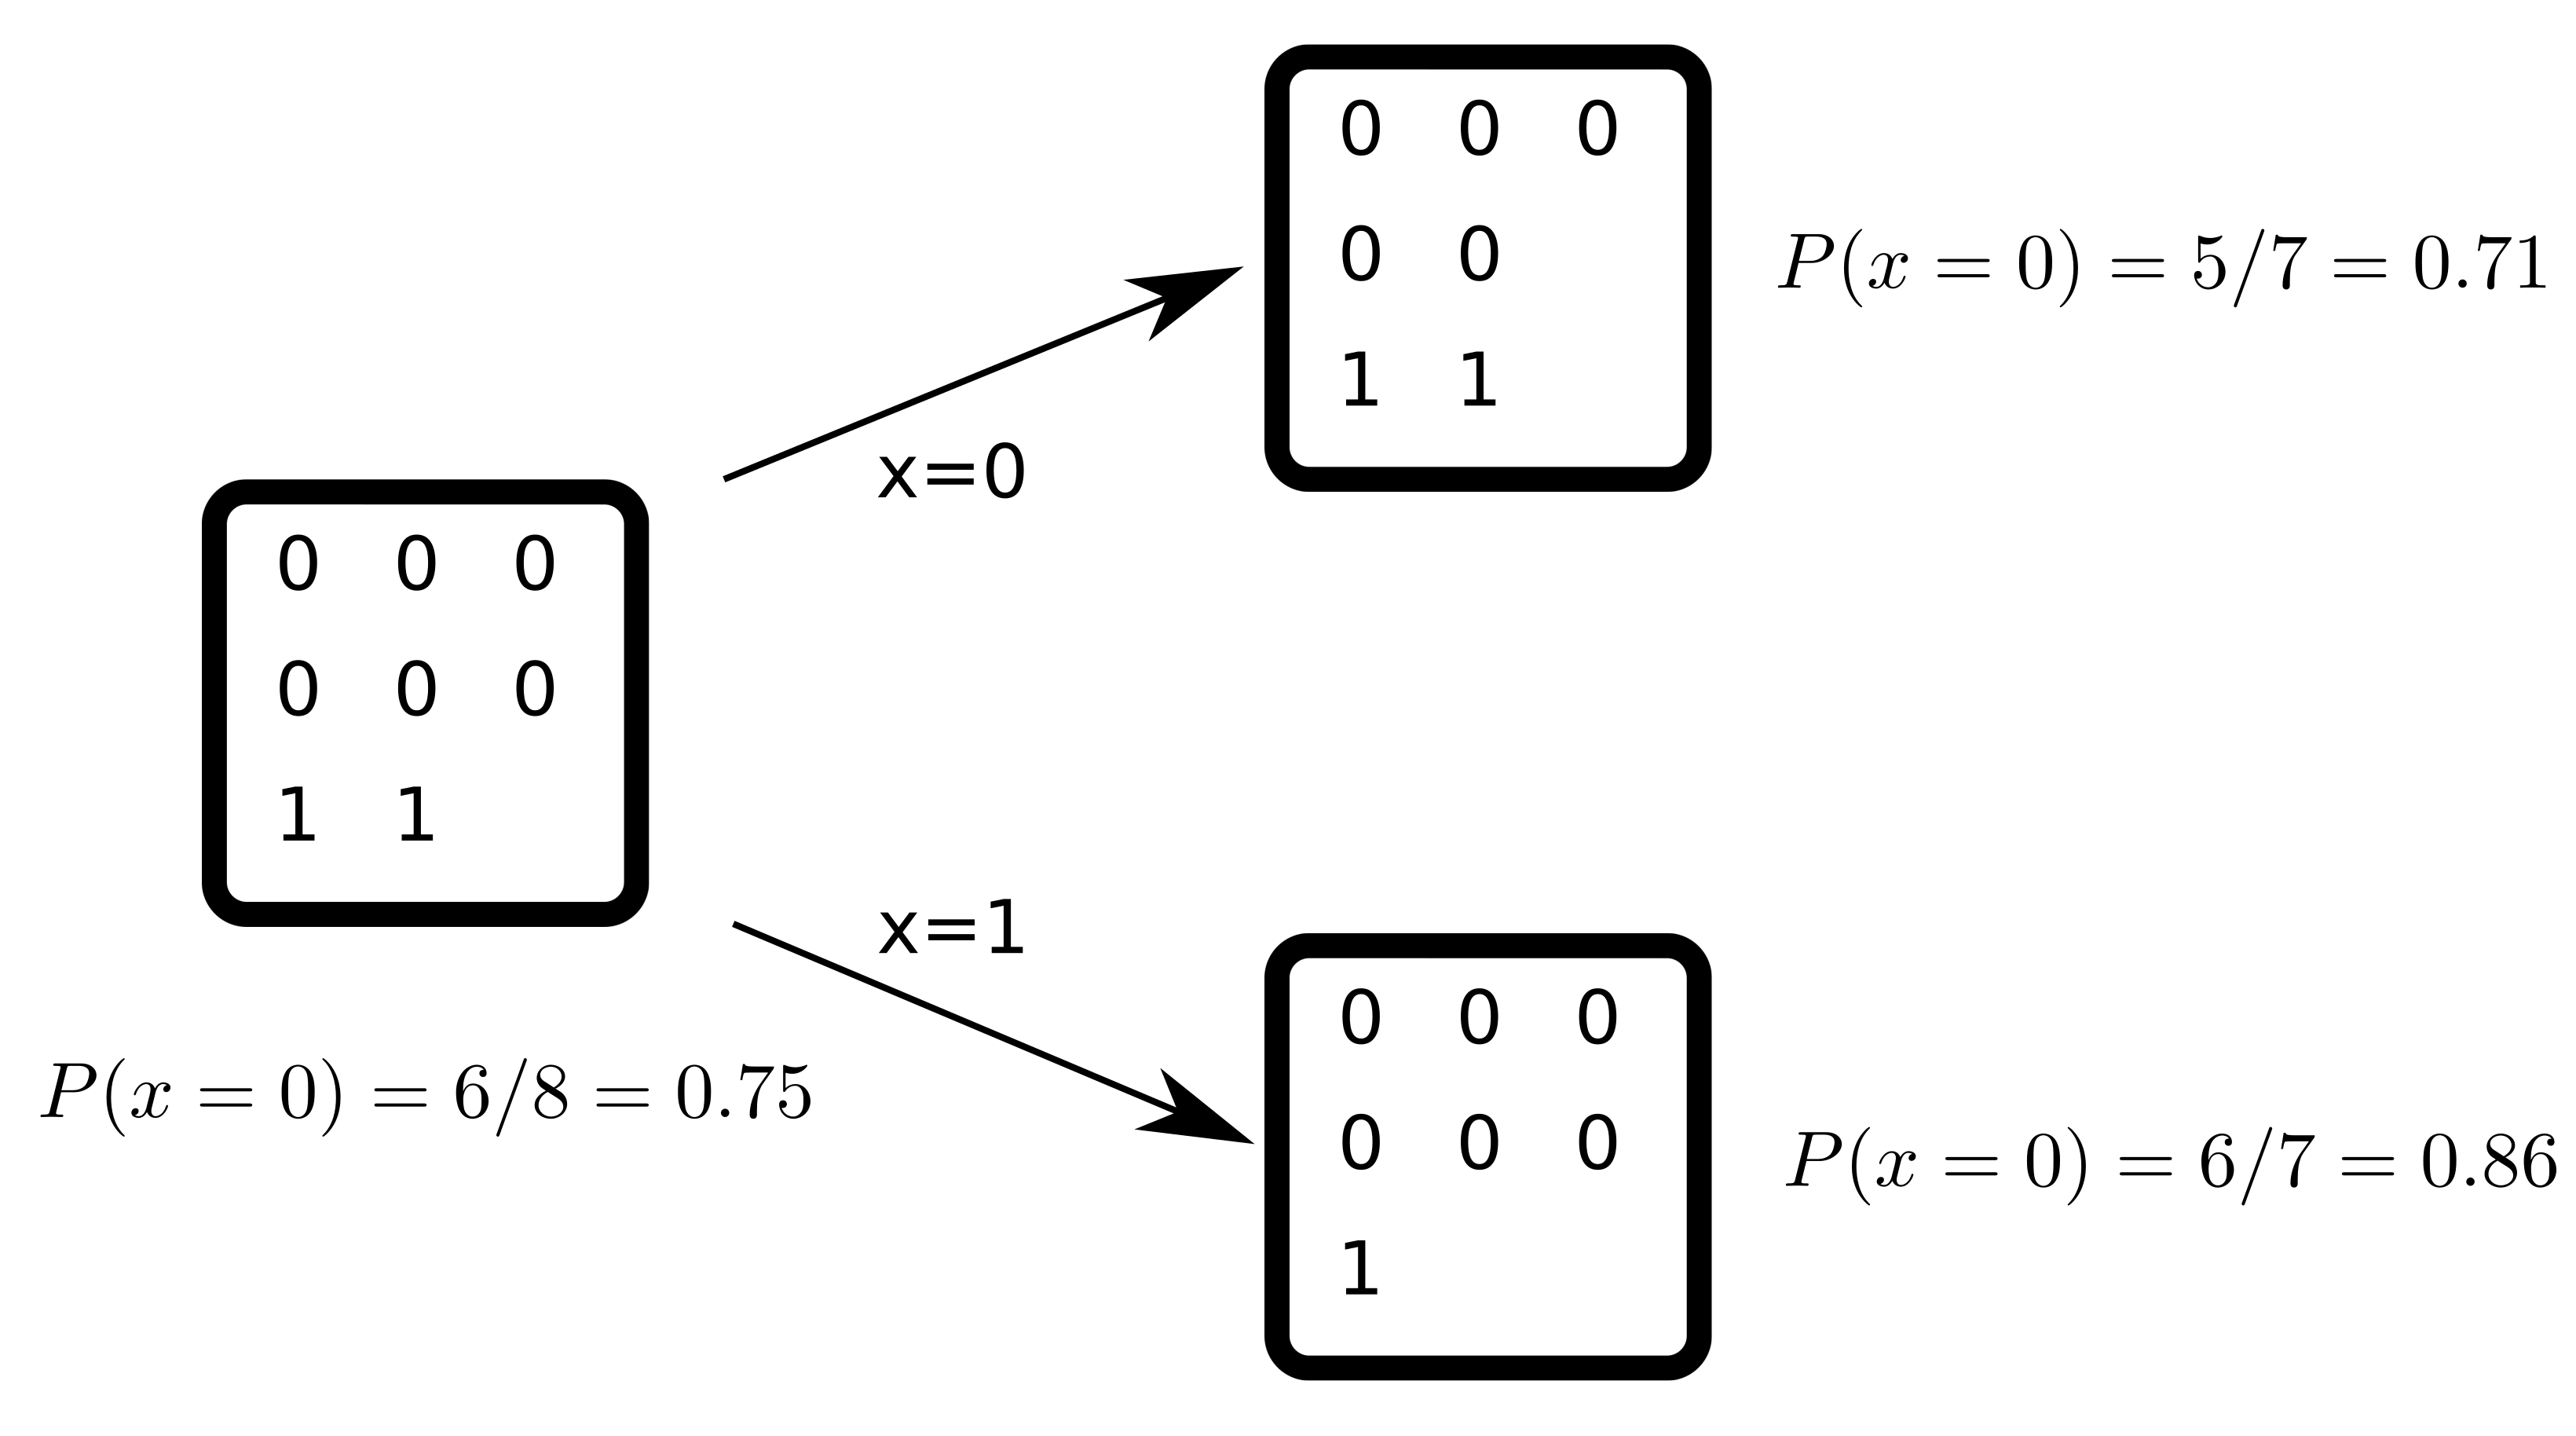
\includegraphics[width=0.70\paperwidth]{Diagramas/bag.png}%
   \end{figure}
\end{frame}

\begin{frame}{Calculo de intervalo de salida del bloque codificador}
\begin{itemize}
    \item Se utiliza el concepto de `escalado' propuesto en \cite[Sec.\ 4] {schulte}
    \item Permite aumentar los límites de los subintervalos cuando estos cumplen con las siguientes condiciones:
\begin{itemize}
    \item Si $u_s \leq 0.5$:
        \begin{itemize}
            \item $u_s' = 2 * u_s$
            \item $l_s' = 2 * l_s$
            \item $l_i' = 2 * l_i$
        \end{itemize}
    \item Si $l_s > 0.5$: 
        \begin{itemize}
            \item $u_s' = 2 * (u_s - 0.5)$
            \item $l_s' = 2 * (l_s - 0.5)$
            \item $l_i' = 2 * (l_i - 0.5)$
        \end{itemize}
    \end{itemize}
    \item Esto permitirá optimizar la cantidad de bits en la implementación
\end{itemize}
\end{frame}

%\begin{frame}{Calculo de intervalo de salida de bloque codificador}
%Para obtener una probabilidad $P_{(x=0)}=0.75$:
%\begin{enumerate}
%    \item Se inicializa la bolsa con ocho bits de los cuales dos son `1'
%    \item Se inicializan los limites superior e inferior: $u_s=1.0$ y $l_s=0.0$
%    \item Se selecciona un subintervalo en base al limite del intervalo de entrada $l_i$ y se asigna un bit a la salida ($Xo_{cod}$)
%    \begin{itemize}
%        \item Si  $l_i \geq v_m \implies [0,75;1,0)\ , \ Xo_{cod}=1 $ 
%        \item Si  $Xl_i < v_m \implies (0,0;0,75]\ , \ Xo_{cod}=0 $ 
%    \end{itemize}
%    \item Si es necesario se realiza escalado de valores $u_s$, $l_s$ y $l_i$
%    \item Se elimina bit $Xo_{cod}$ de la bolsa y se recalcula $P_{(x=0)}$
%    \item Este proceso se repite tantas veces como bits de salidia se tengan
%\end{enumerate}
%\end{frame}

\begin{frame}{Ejemplo de calculo de intervalo de salida del bloque codificador}
\begin{figure}
  \centering
  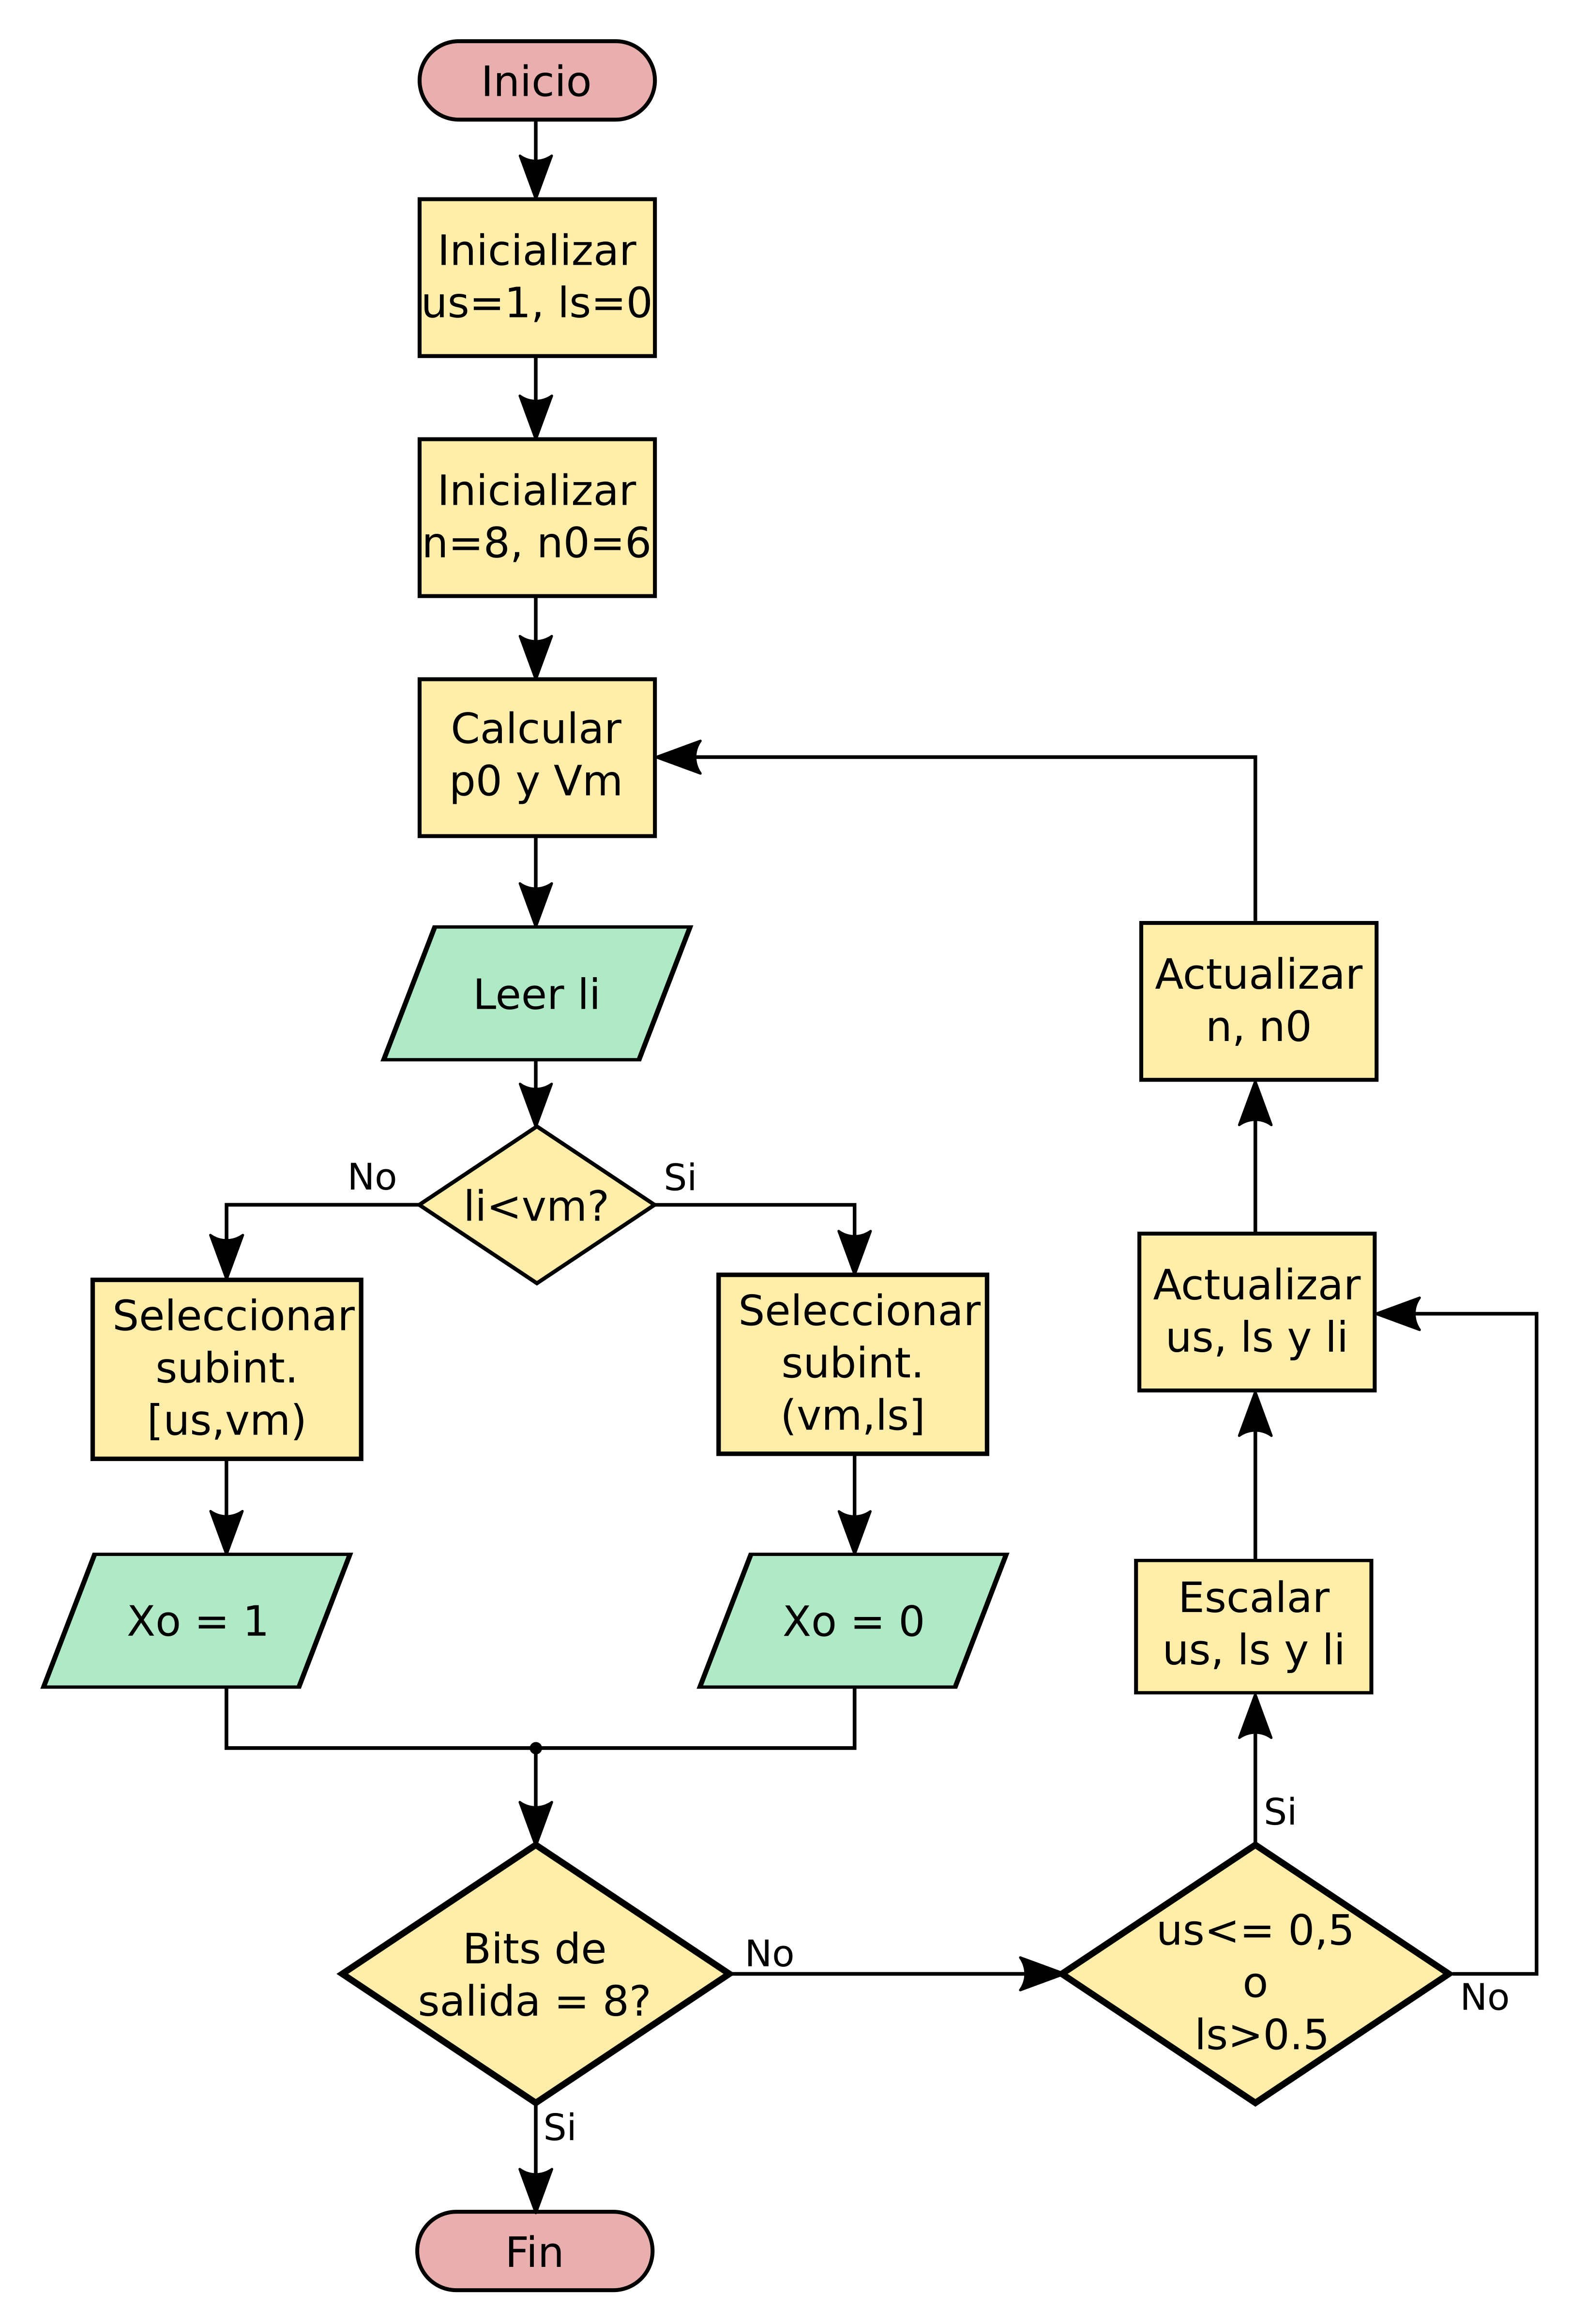
\includegraphics[ height=0.85\textheight]{Diagramas/diag_cisc.png}%
   \end{figure}
\end{frame}

\begin{frame}{Ejemplo de calculo de intervalo de salida del bloque codificador}
Para $Xi_{cod} = 1010$ y  $P_{(x=0)}=0.75$:
    \begin{figure}[H]
  \centering
  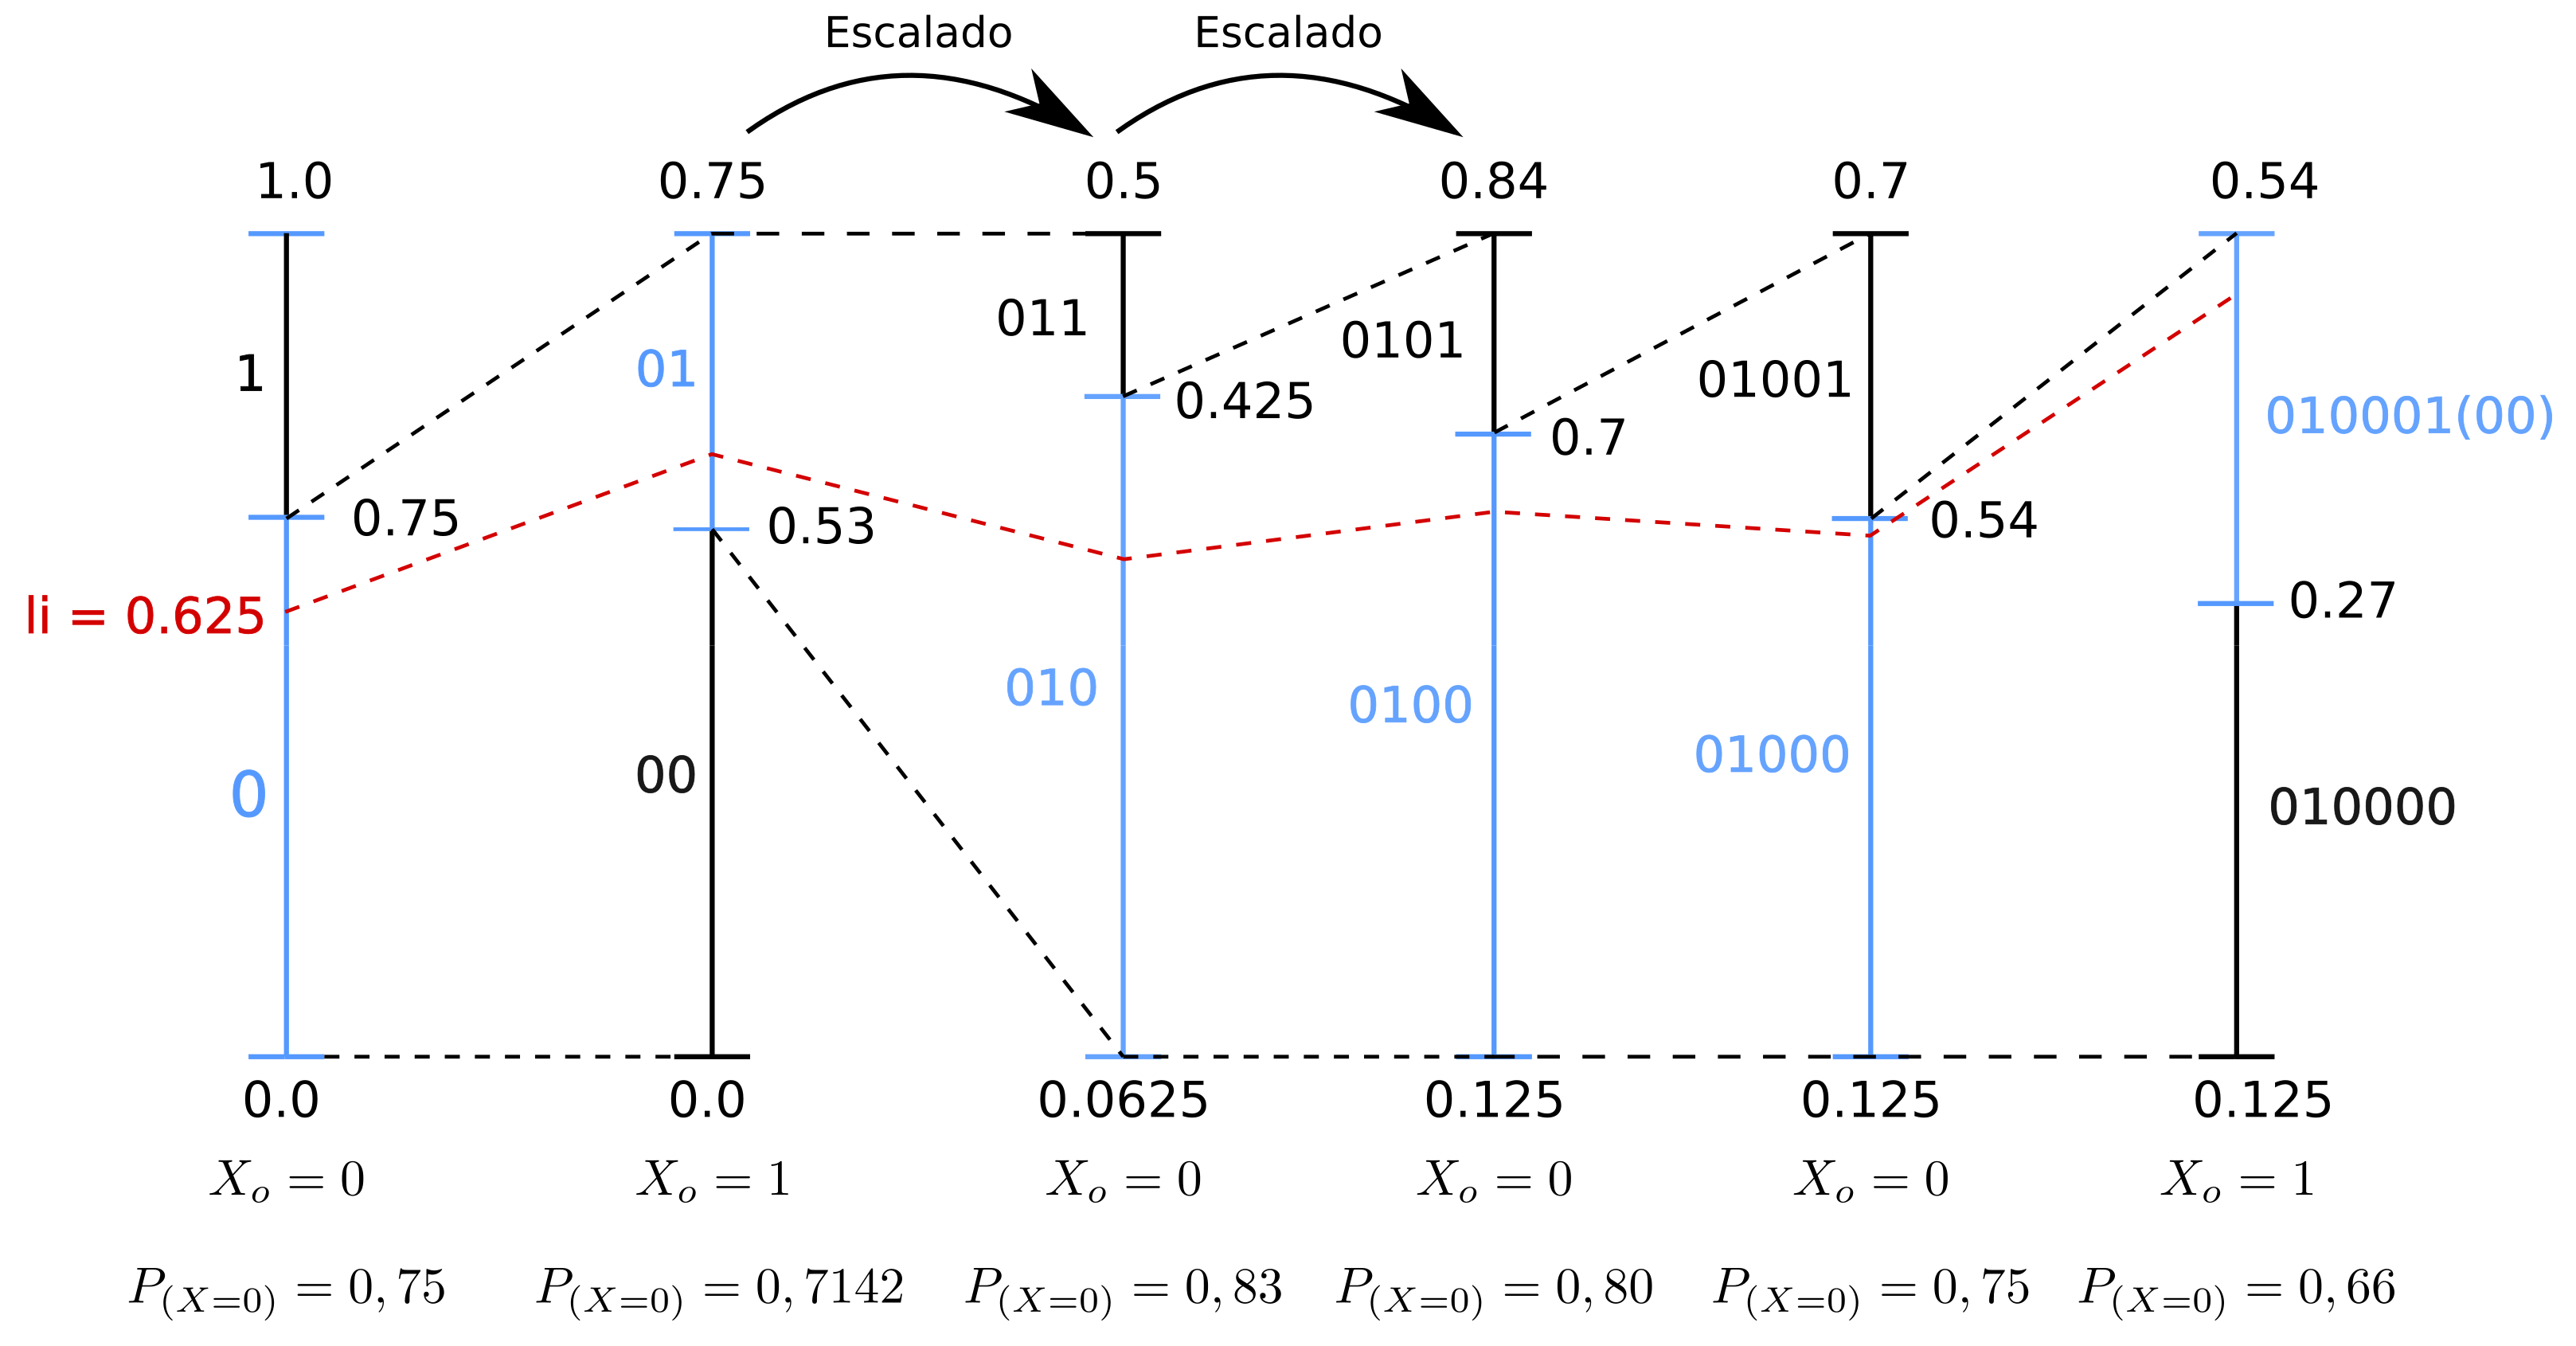
\includegraphics[width=0.85\paperwidth]{Diagramas/int_sal_cod.png}%
   \end{figure}
\end{frame}

\begin{frame}{Intervalos codificados}
 Siguiendo estos pasos para cada una de las posibles secuencias de entrada:
 
 \begin{table}[H]
\centering
\adjustbox{max height=\dimexpr\textheight-5.5cm\relax,
           max width=\textwidth}{\begin{tabular}{|c|c|}
\rowcolor{gray!50}
\hline
$Xi_{cod}$ & $Xo_{cod}$ \\ \hline
0000         &  00000011         \\ \hline
0001         &  00000101         \\ \hline
0010         &  00001001         \\ \hline
0011         &  00001100         \\ \hline
0100         &  00010010         \\ \hline
0101         &  00010100         \\ \hline
0110         &  00100001         \\ \hline
0111         &  00100100         \\ \hline
1000         &  00110000         \\ \hline
1001         &  01000001         \\ \hline
1010         &  01000100         \\ \hline
1011         &  01010000         \\ \hline
1100         &  10000001         \\ \hline
1101         &  10000010         \\ \hline
1110         &  10001000         \\ \hline
1111         &  10100000         \\ \hline
\end{tabular}}
\end{table}


\end{frame}

\begin{frame}{Calculo de intervalo de entrada del bloque decodificador}
\begin{itemize}
    \item Este proceso  es similar al calculo de intervalo de entrada del codificador.
    \item En este caso la secuencia de entrada no posee una distribución uniforme.
    \item Toma como entrada una secuencia de 8 bits. 
    \item Se toma como salida el limite superior del subintervalo final $u_s$, el cual es necesario para el calculo del intervalo de salida.
\end{itemize}
\end{frame}

\begin{frame}{Ejemplo de calculo de intervalo de entrada del bloque decodificador}
Para $Xi_{cod} = 01000100$ y  $P_{(x=0)}=0.75$:
\begin{figure}[H]
  \centering
  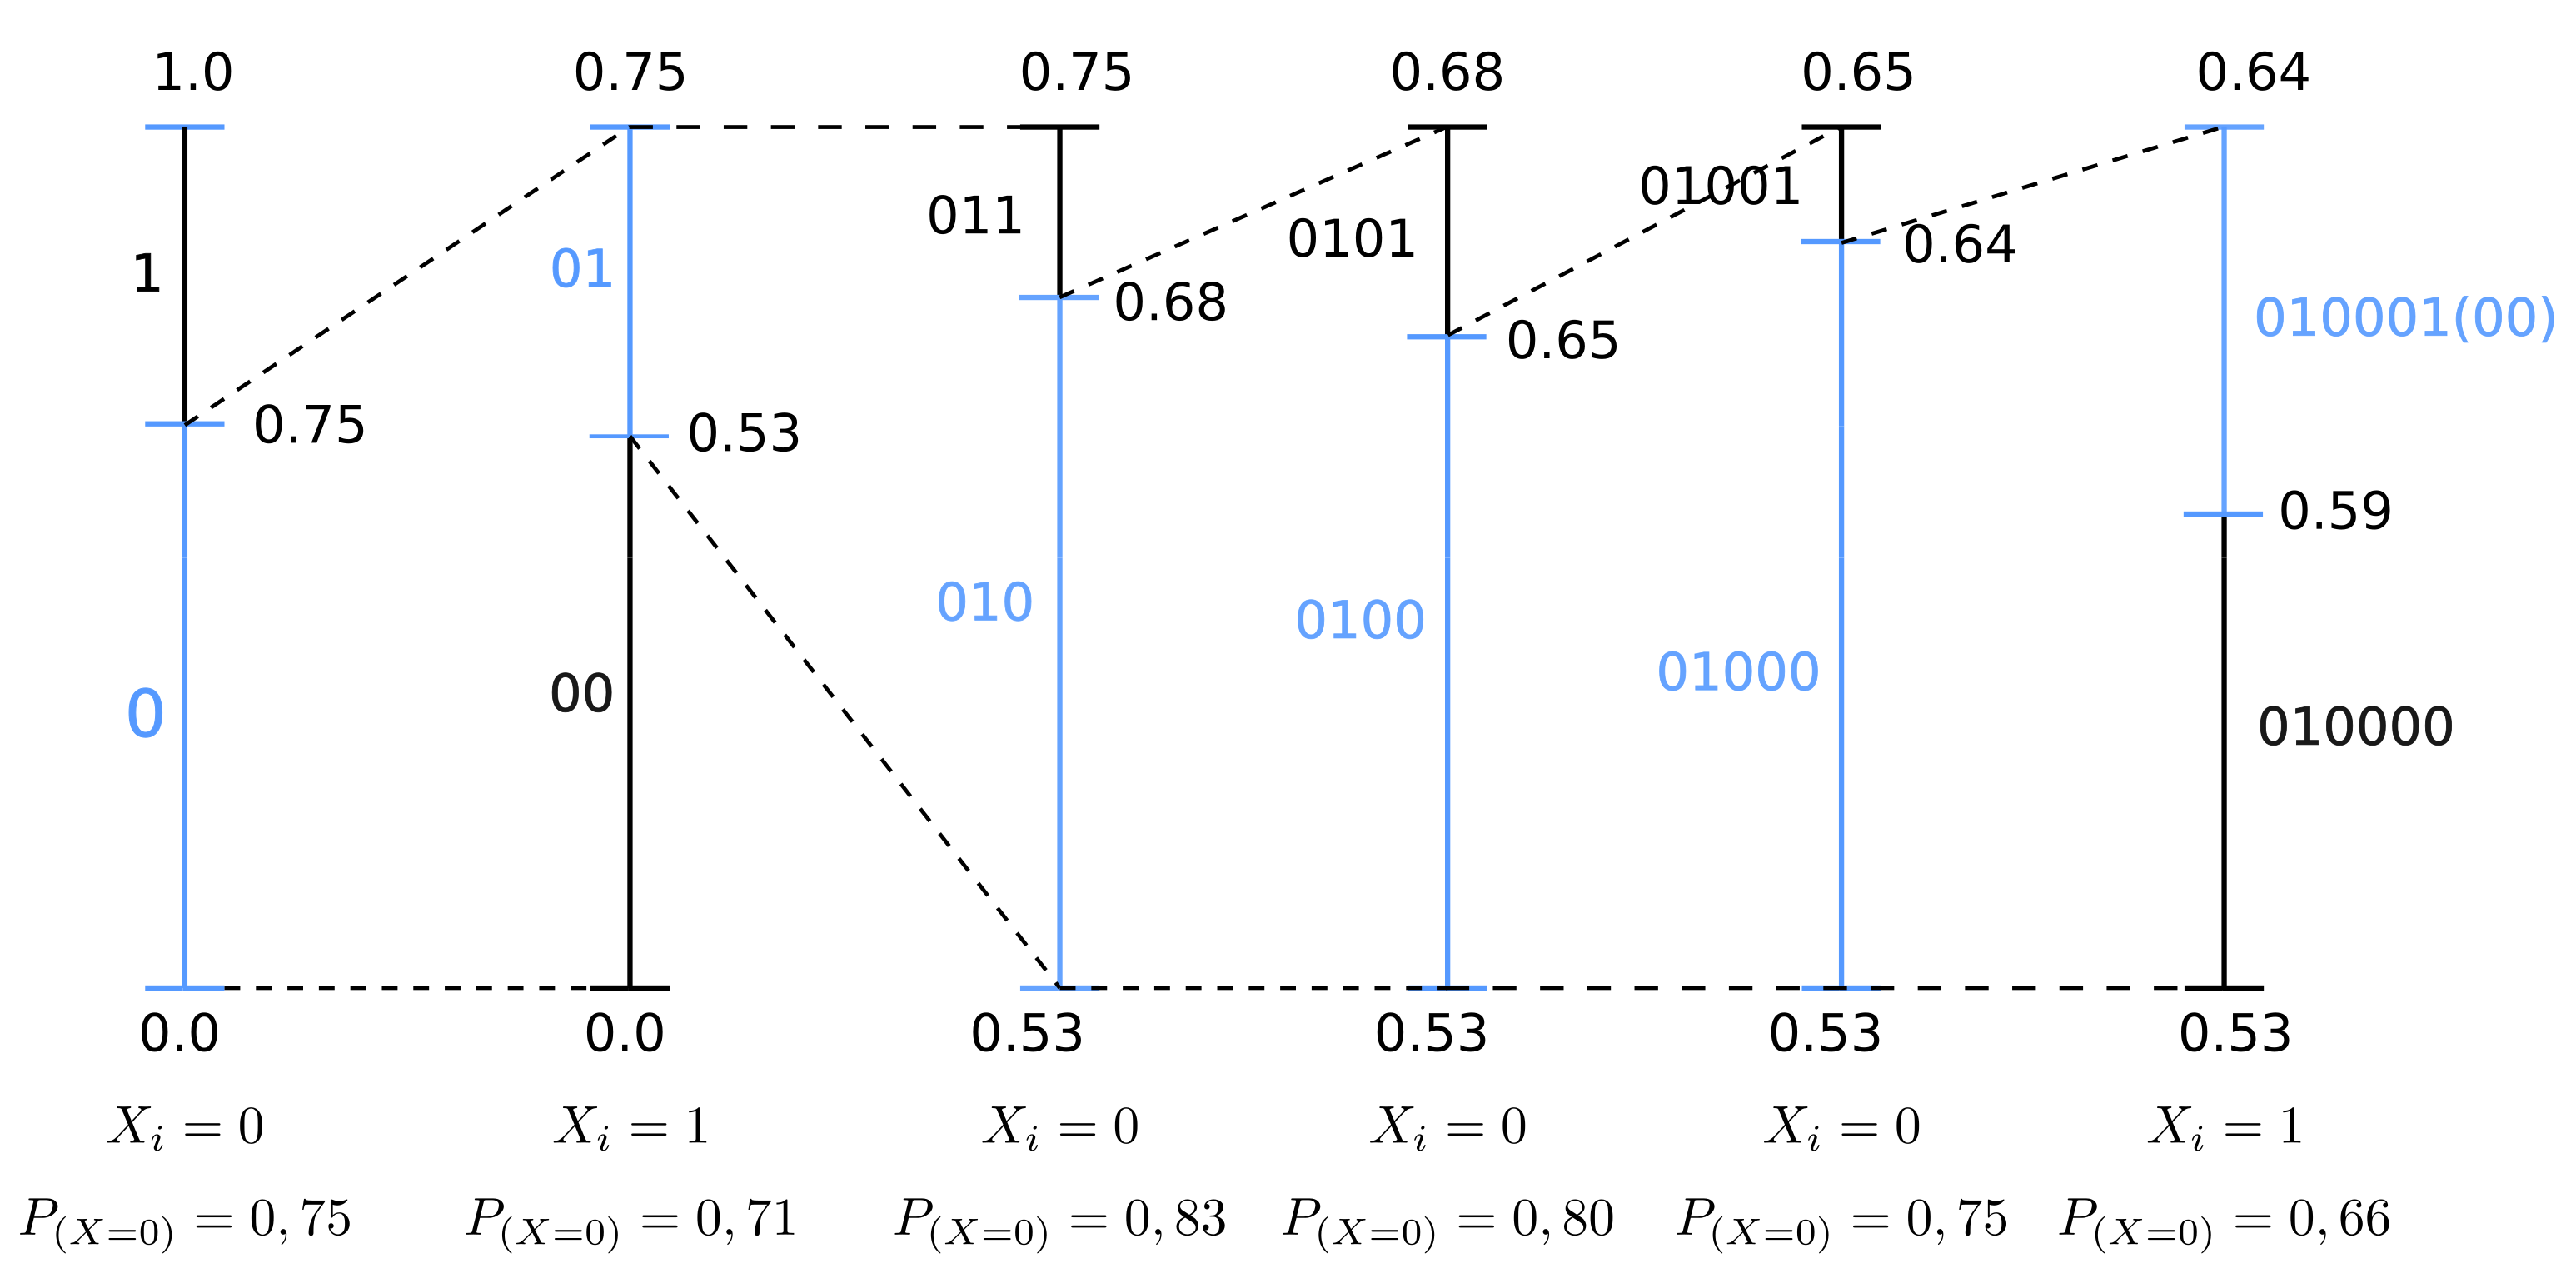
\includegraphics[width=0.85\paperwidth]{Diagramas/int_ent_dec.png}%
\end{figure}
\end{frame}

\begin{frame}{Calculo de intervalo de salida del bloque decodificador}
\begin{itemize}
    \item Este proceso  es similar al calculo de intervalo de salida del codificador.
    \item  En este caso la secuencia de salida posee una distribución uniforme.
    \item  Se tienen cuatro bits de salida.
    \item Se toma como entrada el limite superior del subintervalo final $u_s$
\end{itemize}
\end{frame}

\begin{frame}{Ejemplo de calculo de intervalo de salida de bloque decodificador}
Para $Xi_{cod} = 01000100$ y  $P_{(x=0)}=0.75$:
\begin{figure}[H]
  \centering
  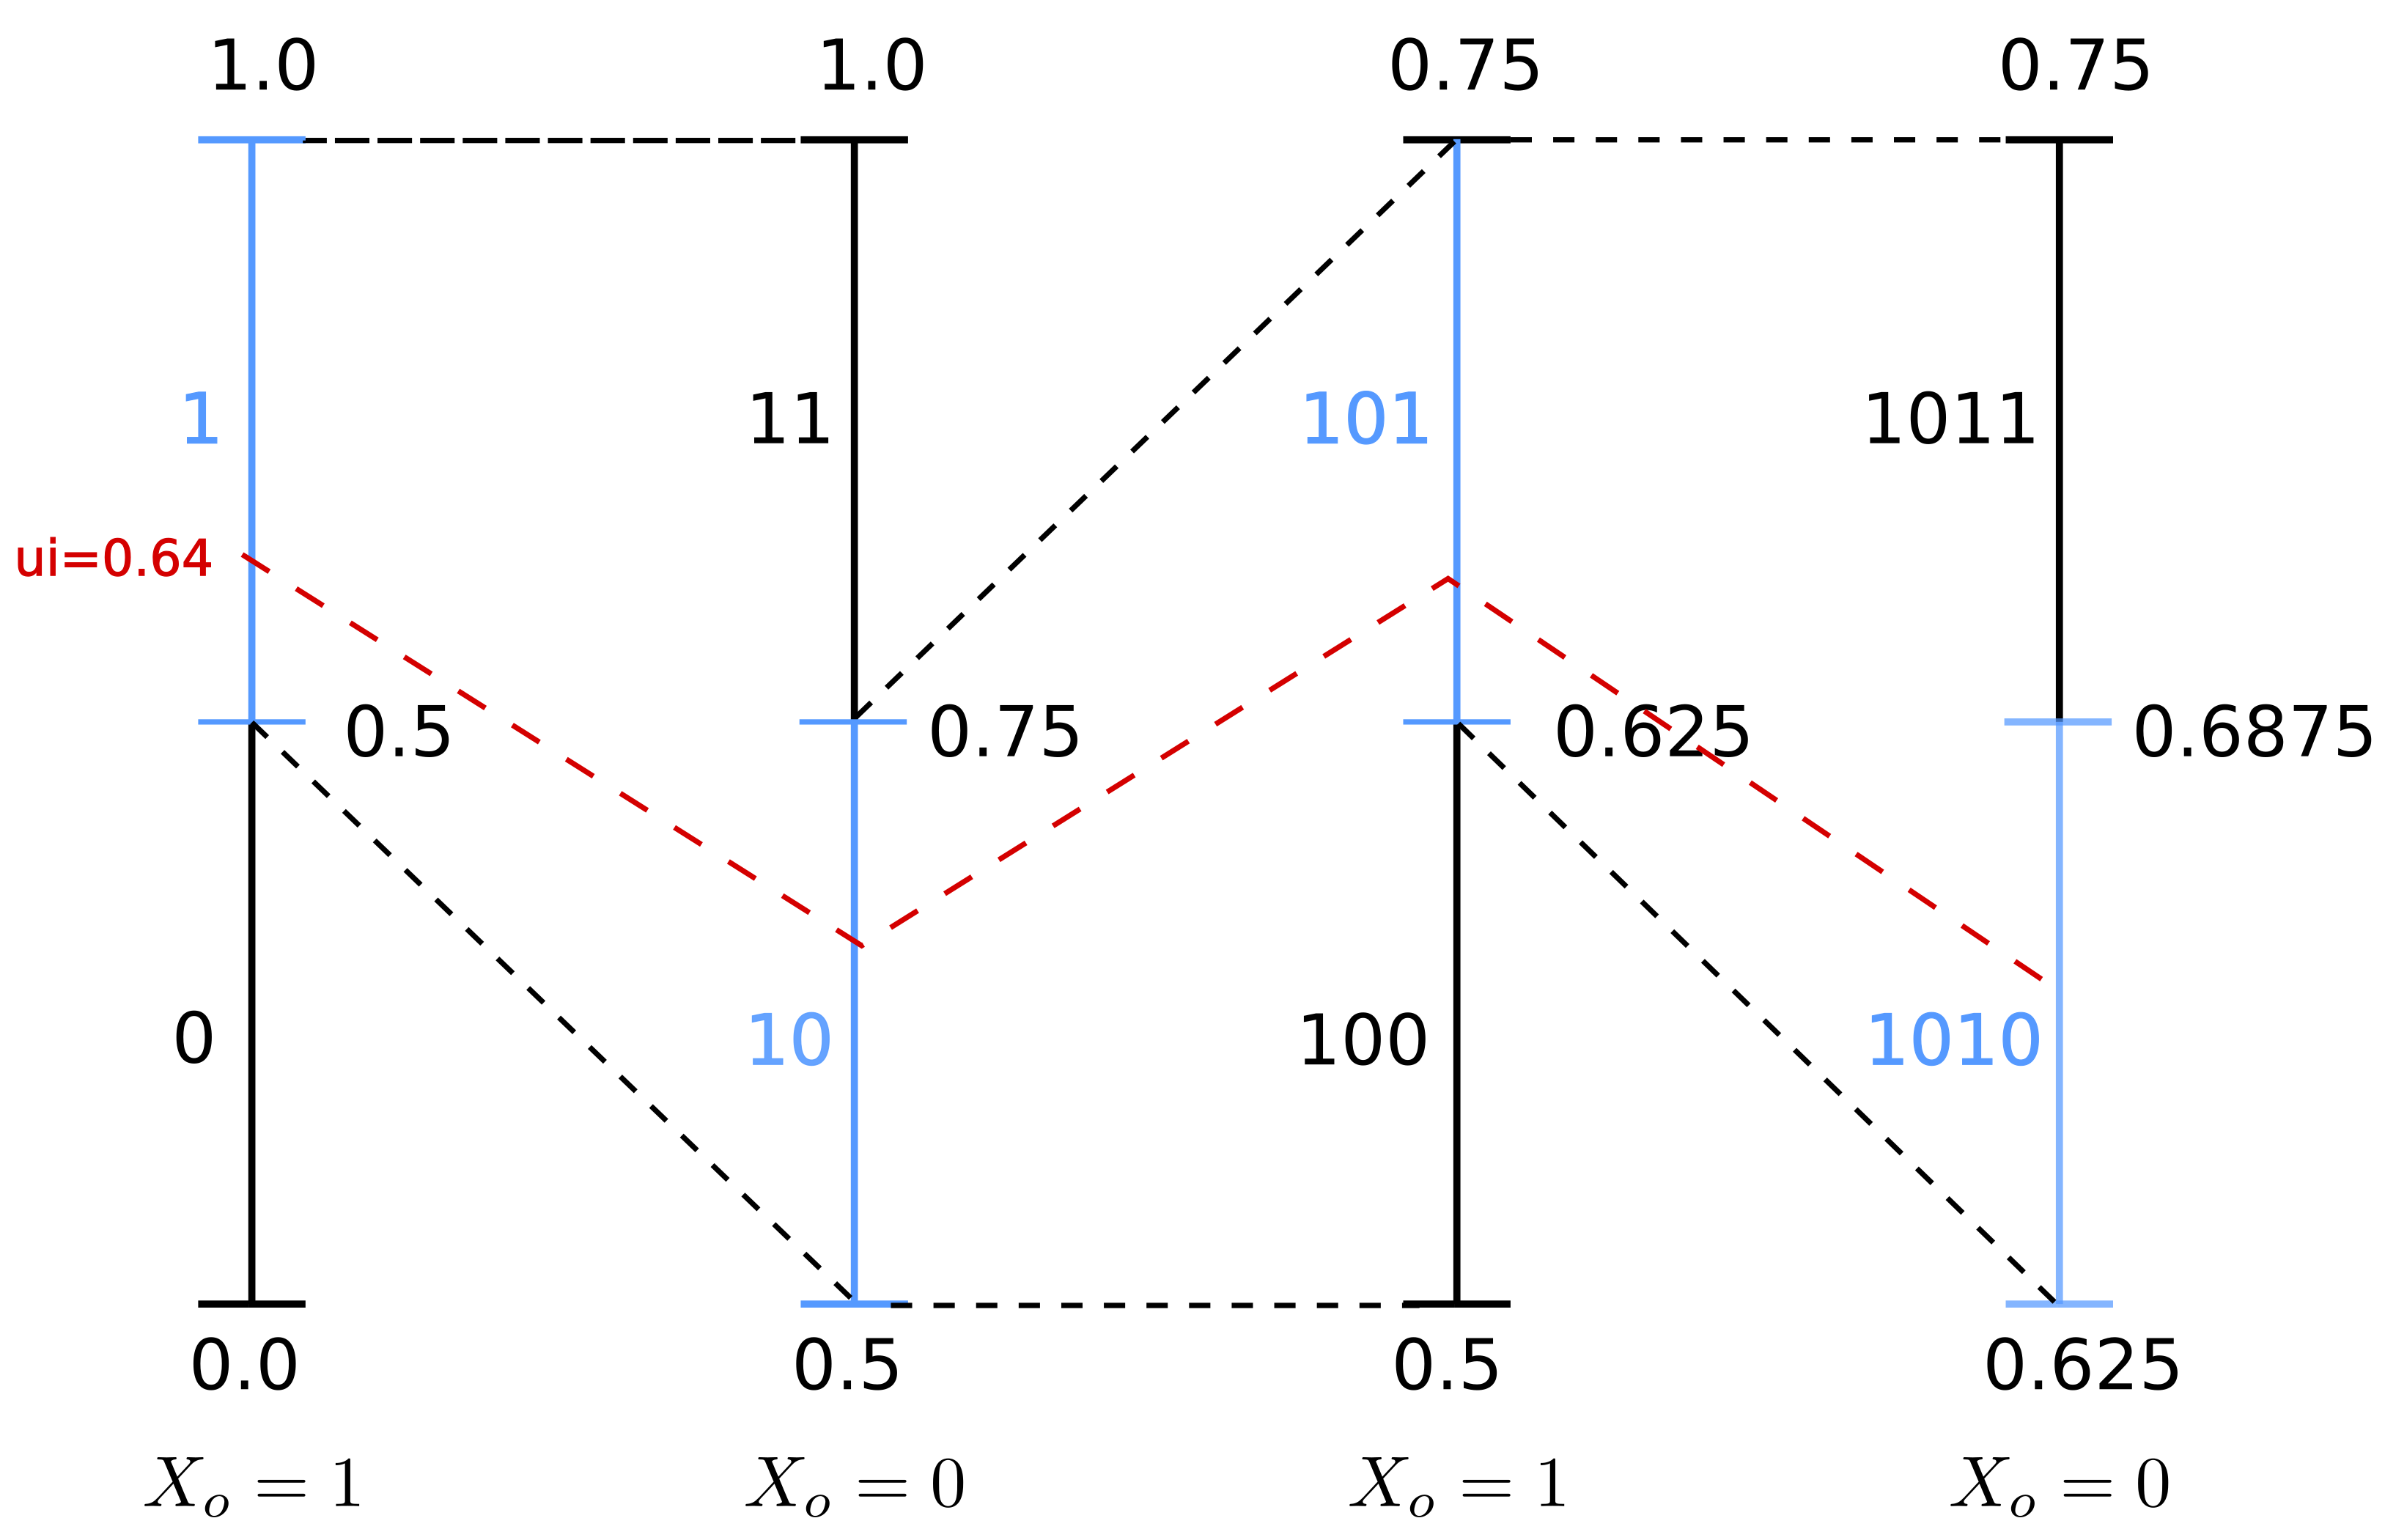
\includegraphics[width=0.70\paperwidth]{Diagramas/int_sal_dec.png}%
\end{figure}
\end{frame}

\subsection{Modelado en punto flotante}

\begin{frame}{Modelando en punto flotante}
\begin{figure}[H]
  \centering
  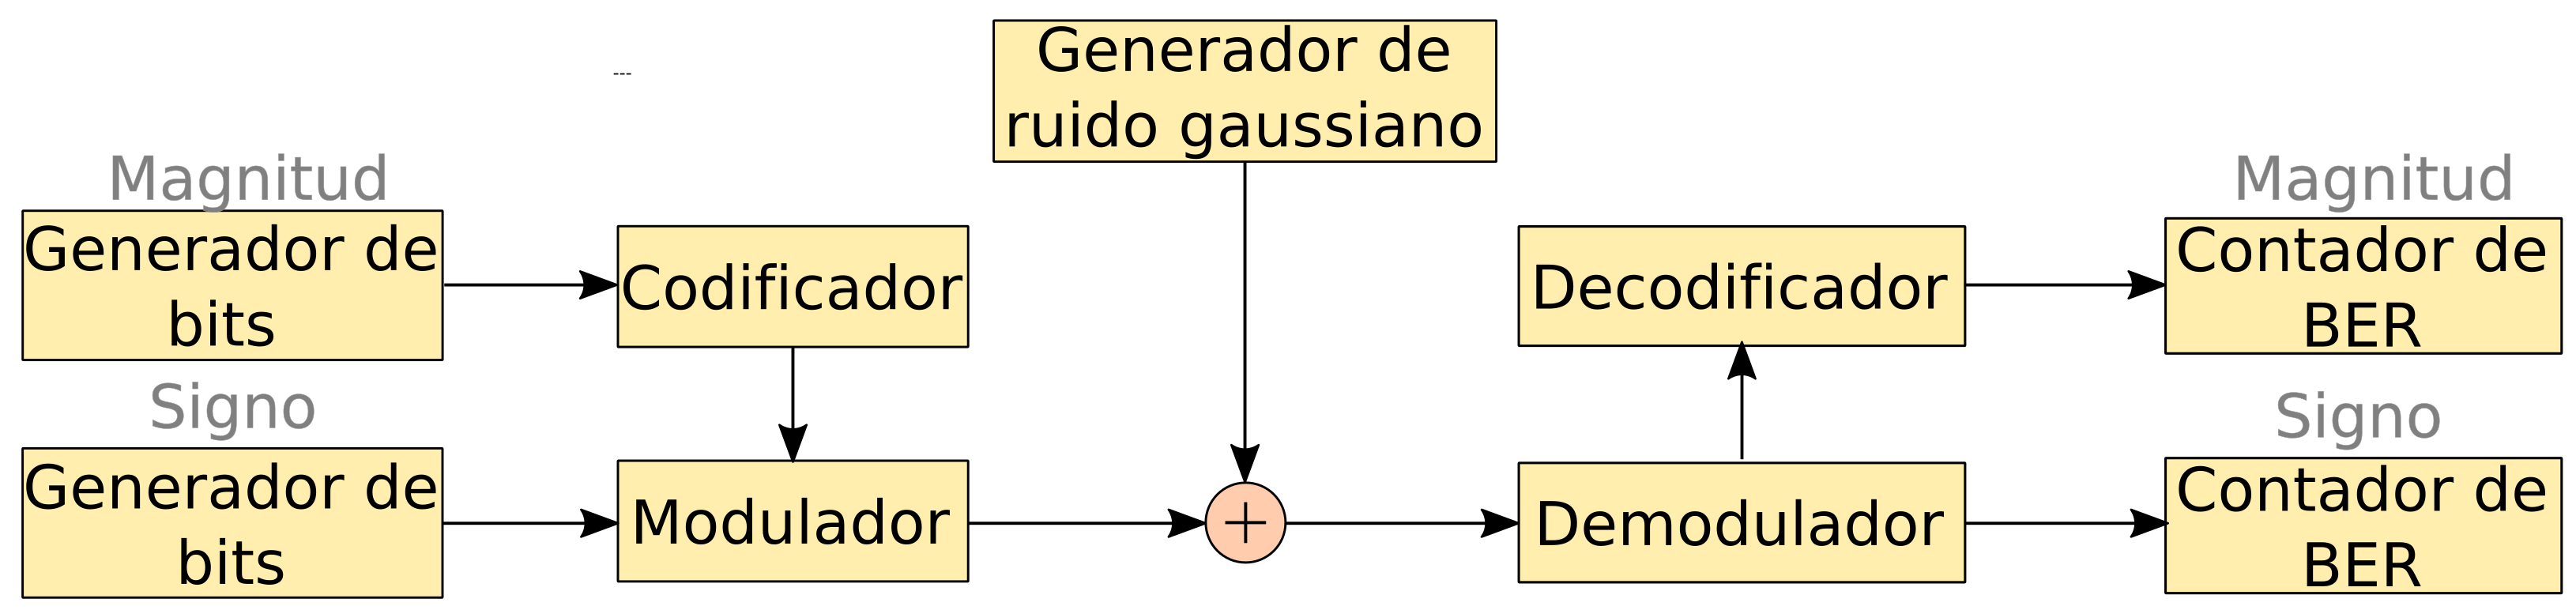
\includegraphics[width=0.85\paperwidth]{Diagramas/proyect_alto_nivel.png}%
\end{figure}
\end{frame}

\begin{frame}{Funcionamiento del codificador}
    \begin{itemize}
        \item Para el calculo del intervalo de entrada:
        
        \begin{itemize}
            \item Calculo del valor medio 
                \begin{equation*}
                    v_{m} = (u_{i} - l_{i}) / 2 + l_{i} 
                \end{equation*}
            \item if $x_{in} == 0$ : return \{$u_{i}$ , $v_{m}$\} \tap  else : return \{$v_{m}$ , $l_{i}$\}
        \end{itemize}
        
        \item Para el calculo del intervalo de salida 
        
        \begin{itemize}
            \item Calculo del valor medio 
                \begin{equation*}
                    v_{m} = (u_{s} - l_{s}) * p_{0} + l_{s} 
                \end{equation*}
            \item if $l_{i} >= v_{m}$ : return \{1 , $u_{s}$ , $v_{m}$\} \tap  else : return \{0, $v_{m}$ , $l_{s}$\}
            \item if $u_{s} <= 0.5\ | \ l_{s} > 0.5$ : escalado()
            \item $n = n-1$ ; if $x == 0$ : $n_{0} = n_{0} - 1$ ; $p{0} = n{0} / n$
        \end{itemize}
    
    \end{itemize}
\end{frame}

\begin{frame}{Resultados obtenidos en punto flotante}
\begin{columns}

    \begin{column}{0.506\paperwidth}
    \begin{figure}
        \centering
        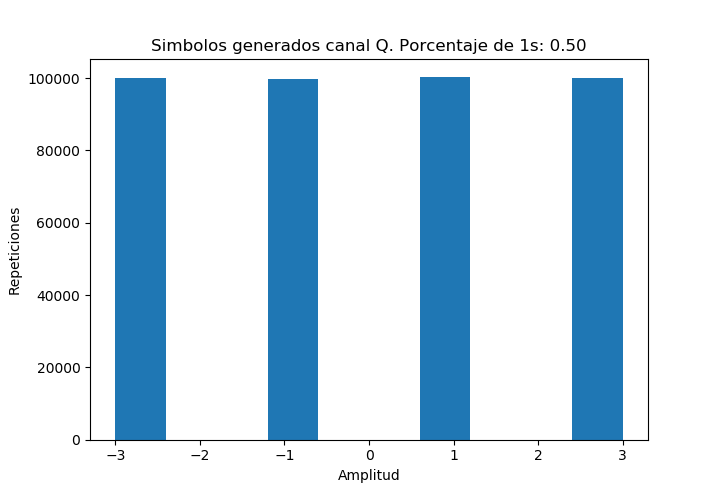
\includegraphics[width=\textwidth]{Graficos/Generated_symbols.png}%
        \caption{Símbolos sin codificar, $P_{(x=0)}=0.5$}
        % \label{fig:my_label}
    \end{figure}
    \end{column}
            

    \begin{column}{0.48\paperwidth}  
    \begin{figure}
        \centering
        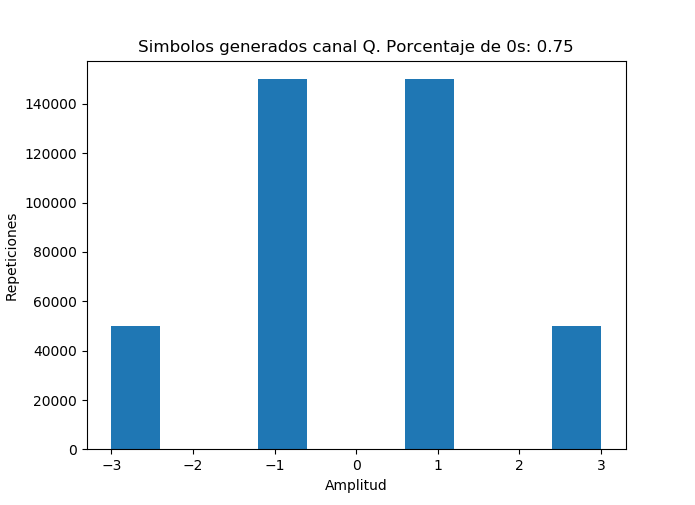
\includegraphics[width=\textwidth]{Graficos/coded_symbols_6.png}
        \caption{Símbolos codificados, $P_{(x=0)}=0.75$}
        %\label{fig:my_label}
    \end{figure}
    \end{column}
    
\end{columns}
\end{frame}

\begin{frame}{Resultados obtenidos en punto flotante}
\begin{columns}

    \begin{column}{0.48\paperwidth}
    \begin{figure}
        \centering
        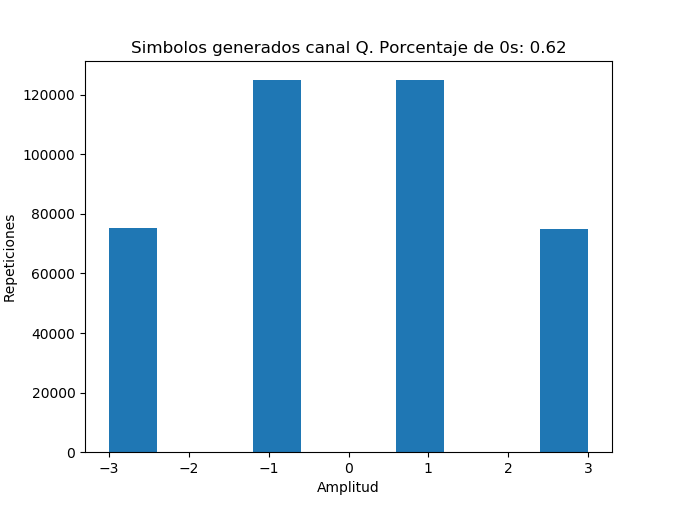
\includegraphics[width=\textwidth]{Graficos/coded_symbols_5.png}
        \caption{Símbolos codificados, $P_{(x=0)}=0.62$}
        \label{fig:my_label}
    \end{figure}
    
    \end{column}
    \begin{column}{0.51\paperwidth}  
    \begin{figure}
        \centering
        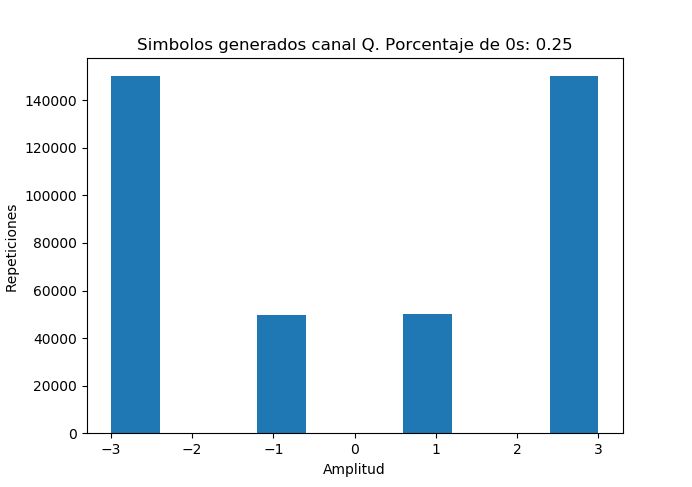
\includegraphics[width=\textwidth]{Graficos/coded_symbols_2.png}
        \caption{Símbolos codificados, $P_{(x=0)}=0.25$}
        \label{fig:my_label}
    \end{figure}

    \end{column}
\end{columns}
\end{frame}

\begin{frame}{Resultados obtenidos en punto flotante}
\begin{columns}

    \begin{column}{0.48\paperwidth}
    \begin{figure}
        \centering
        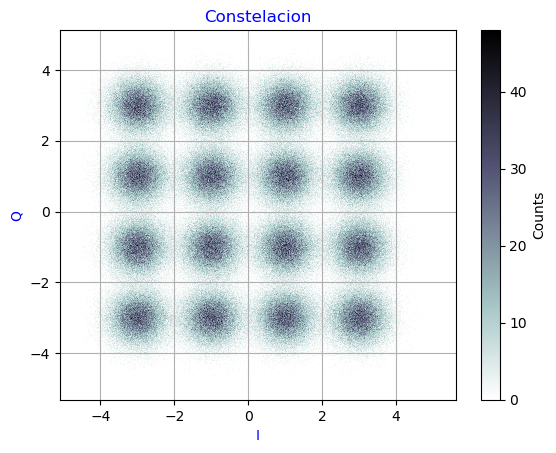
\includegraphics[width=\textwidth]{Graficos/Constellation_05.png}%
        \caption{Símbolos sin codificar, $P_{(x=0)}=0.5$}
        \label{fig:my_label}
    \end{figure}
    
    \end{column}
    \begin{column}{0.48\paperwidth}  
    
    \begin{figure}
        \centering
        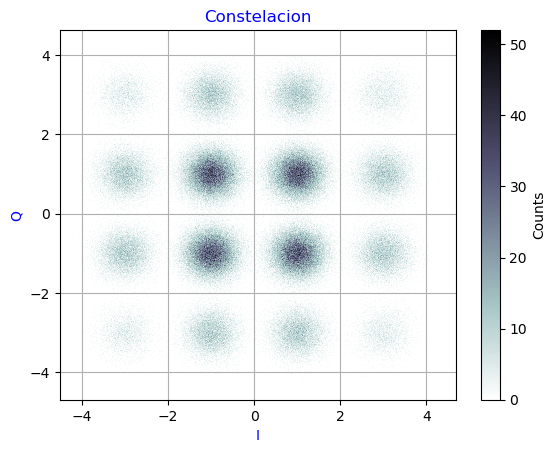
\includegraphics[width=\textwidth]{Graficos/Constellation_025.png}
        \caption{Símbolos codificados, $P_{(x=0)}=0.75$}
        \label{fig:my_label}
    \end{figure}
    
    \end{column}
\end{columns}
\end{frame}


\begin{frame}{Resultados obtenidos en punto flotante}
\begin{columns}
    \begin{column}{0.49\paperwidth}
    \small 
    \begin{figure}
        \centering
        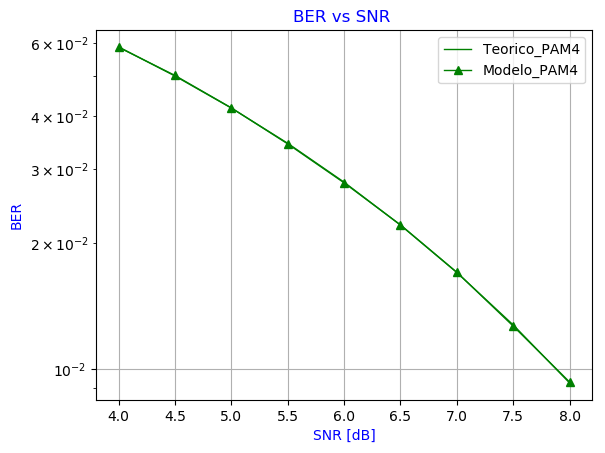
\includegraphics[width=\textwidth]{Graficos/BER_vs_SNR_1.png}%
        \caption{PAM-4 sin codificar}
        \label{fig:my_label}
    \end{figure}
    
    \end{column}
    \begin{column}{0.48\paperwidth}  
    \begin{figure}
        \centering
        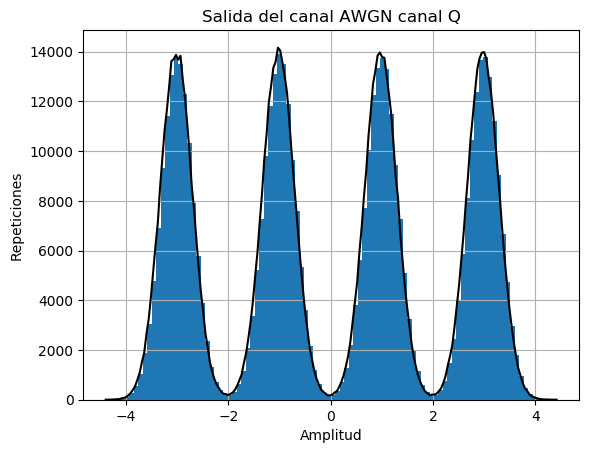
\includegraphics[width=\textwidth]{Graficos/AWGN_symbols.png}
        \caption{Símbolos sin codificar}
        \label{fig:my_label}
    \end{figure}
    % \small 
    
    \end{column}
\end{columns}
\end{frame}


\begin{frame}{Penalidad por redundancia }
\begin{itemize}
    \item Se tendrá que de 16 bits transmitidos solo 12 son de información 
    \item Se produce un desplazamiento en la curva de 
    \begin{equation*}
        10.log(16/12)\approx1,25\, dB
    \end{equation*}
    \item Esto se conoce como `Overhead' (OH)
    \end{itemize}
    \begin{figure}
      \centering
      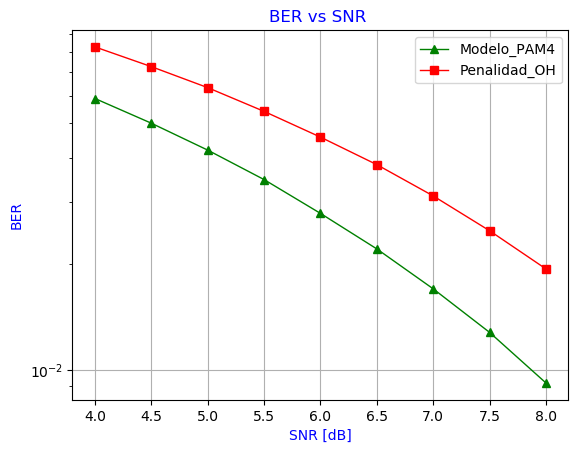
\includegraphics[width=0.55\paperwidth]{Graficos/BER_vs_SNR_2.png}%
    \end{figure}
\end{frame}

\begin{frame}{Ganancia por potencia}
\begin{itemize}
    \item La potencia transmitida está dada por:
    \begin{equation*}
        P_{tx} = P_{(s = 1)}  (1)^{2} + P_{(s = 3)}  (3)^{2}
    \end{equation*}
    \item Para $ P_{(s = 3)}=0.25$ se obtiene una reducción de potencia del 40\% respecto a $ P_{(s = 3)}=0.50$.
    \item SNR constante. 
    \end{itemize}
\begin{figure}
  \centering
  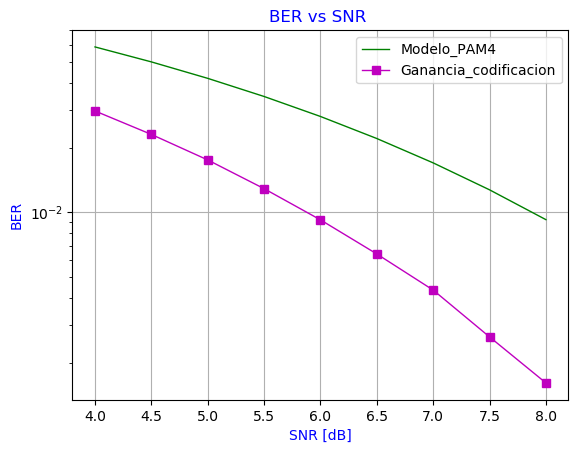
\includegraphics[width=0.55\paperwidth]{Graficos/BER_vs_SNR_3.png}%
\end{figure}
\end{frame}

\begin{frame}{Multiplicación de errores}
\begin{itemize}
    \item Un error de un bit transmitido puede verse reflejado en hasta 4 bits a la salida
 del decodificador
 \item Considerando este efecto, el sistema presenta un mejor desempeño que un sistema PAM-4 para una SNR mayor a 7dB.
 \end{itemize}
 
  \vspace{0.5cm}
\begin{columns}
    \begin{column}{0.48\paperwidth}
    \begin{figure}
        \centering
        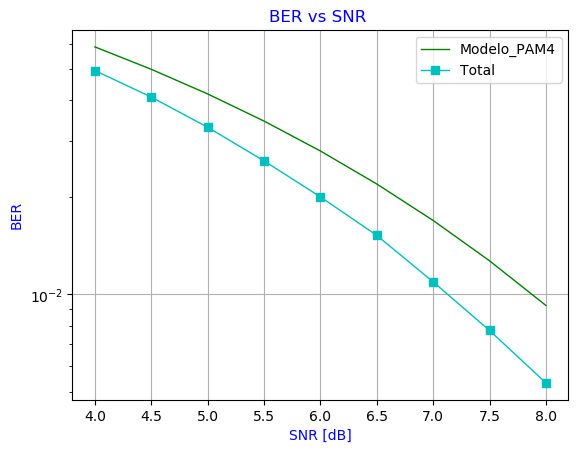
\includegraphics[width=\textwidth]{Graficos/BER_vs_SNR_4.png}%
        \caption{Suma total de efectos}
        \label{fig:my_label}
    \end{figure}
    
    
    \end{column}
    \begin{column}{0.48\paperwidth}  
    
    \begin{figure}
        \centering
        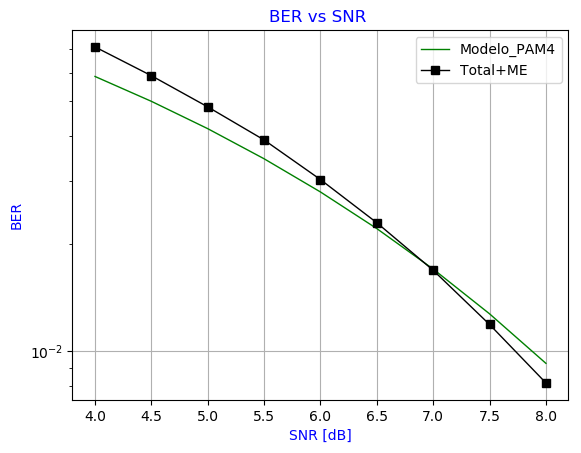
\includegraphics[width=\textwidth]{Graficos/BER_vs_SNR_5.png}
        \caption{Suma de efectos + errores}
        \label{fig:my_label}
    \end{figure}
    
    \end{column}
\end{columns}
% \begin{figure}
%   \centering
%   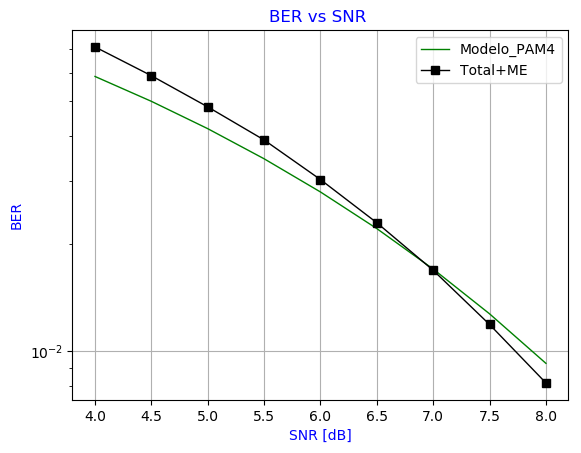
\includegraphics[width=0.55\paperwidth]{Graficos/BER_vs_SNR_5.png}%
% \end{figure}
\end{frame}

\begin{frame}{Modelo final}
Solo se tienen en cuenta los efectos:
\begin{itemize}
    \item Disminución de potencia
    \item Penalidad por redundancia 
 \end{itemize}
 
 
 \vspace{0.5cm}
\begin{columns}
    \begin{column}{0.48\paperwidth}
    \begin{figure}
        \centering
        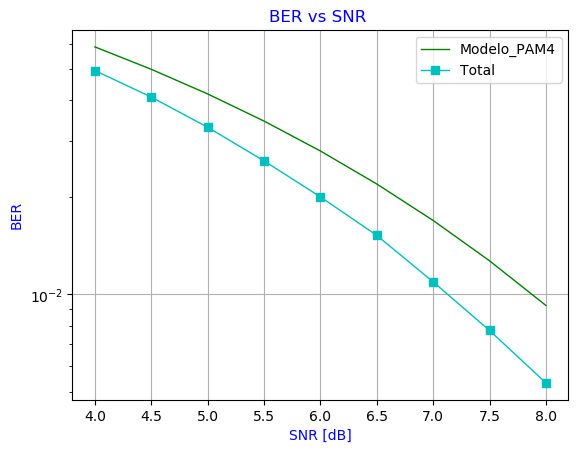
\includegraphics[width=\textwidth]{Graficos/BER_vs_SNR_4.png}%
        \caption{Comparación con PAM-4 teórica}
        \label{fig:my_label}
    \end{figure}
    
    
    \end{column}
    \begin{column}{0.48\paperwidth}  
    
    \begin{figure}
        \centering
        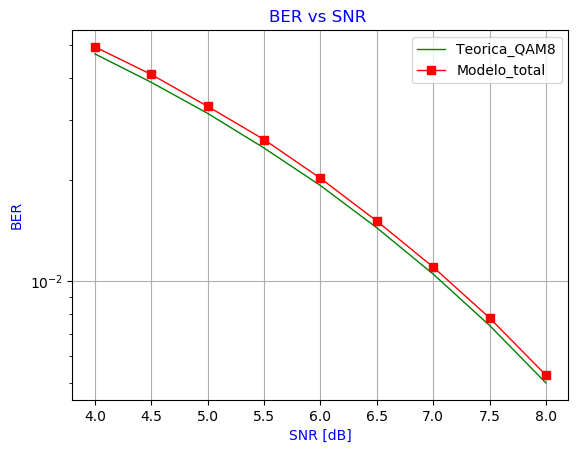
\includegraphics[width=\textwidth]{Graficos/BER_vs_SNR_6.png}
        \caption{Comparación con QAM-8 teórica}
        \label{fig:my_label}
    \end{figure}
    
    \end{column}
\end{columns}
\end{frame}

\begin{frame}{Modelo final}
Si se considera:
\begin{itemize}
    \item Secuencia de entrada de 100 bits 
    \item Probabilidad de $P_{(s=3)} = 0.12$
    \item Se mantiene la misma redundancia
 \end{itemize}
 \begin{figure}
  \centering
  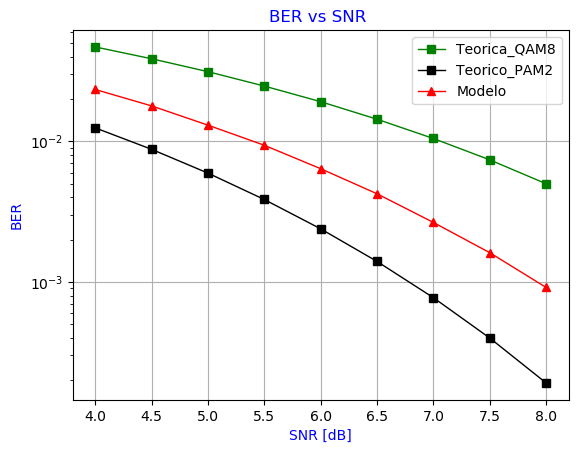
\includegraphics[width=0.6\paperwidth]{Graficos/BER_vs_SNR_8.png}%
\end{figure}
\end{frame}

\begin{frame}{Umbral de decisión}
    \begin{itemize}
        \item En el caso que $P_{(s=1)} \neq P_{(s=3)}$ el umbral óptimo esta dado por:
            \begin{equation}
            P_{(s=1)} exp{(\frac{-(\tau-1)}{2{\sigma}^{2}})} =  P_{(s=3)} exp{(\frac{-(\tau-3)}{2{\sigma}^{2}})}
            \end{equation}
    \item Donde:
    \begin{description}
    \item [$\tau:$] Umbral de decisión
    \item [$\sigma^2:$] Varianza del ruido
    \end{description}
    \item Para $P_{(s=1)}=0.75$ y $P_{(s=3)}=0.25$ :
    \begin{equation*}
         \tau = 2 + 0.55  {\sigma}^{2}
    \end{equation*}
    \end{itemize}
\end{frame}

\begin{frame}{Umbral de decisión}
\begin{columns}
    \begin{column}{0.48\paperwidth}
    \begin{figure}
        \centering
        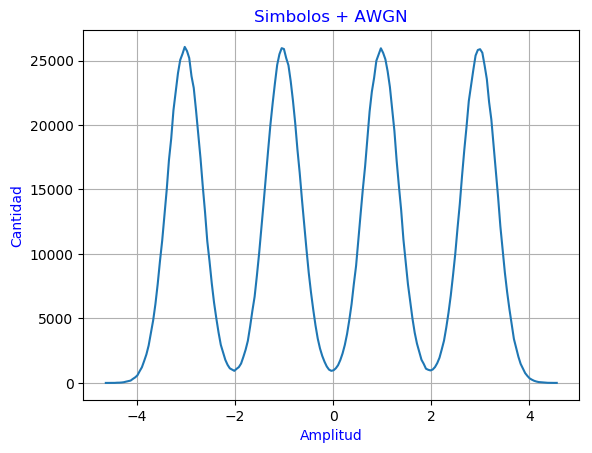
\includegraphics[width=\textwidth]{Graficos/Simbolos_05.png}%
        \caption{Símbolos sin codificar, $P_{(s=1)}=0.5$}
        \label{fig:my_label}
    \end{figure}
    
    \end{column}
    \begin{column}{0.48\paperwidth}  
    
    \begin{figure}
        \centering
         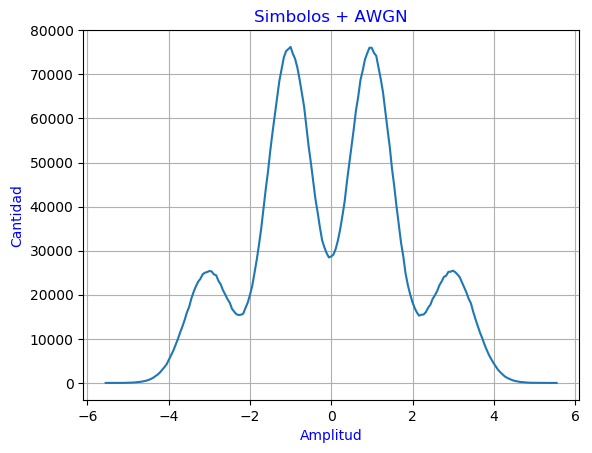
\includegraphics[width=\textwidth]{Graficos/Slicer_025.png}
        \caption{Símbolos codificados, $P_{(s=1)}=0.75$}
        \label{fig:my_label}
    \end{figure}
   
    \end{column}
\end{columns}
\end{frame}

\begin{frame}{Umbral de decisión}
\begin{itemize}
    \item Modelo con umbral de decisión original y con el umbral modificado.
\end{itemize}

 \begin{figure}
  \centering
  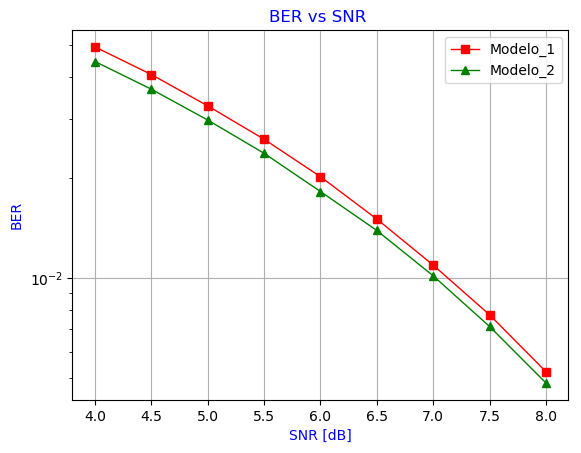
\includegraphics[width=0.70\paperwidth]{Graficos/BER_vs_SNR_9.png}%
\end{figure}
\end{frame}

\subsection{Modelado en punto fijo}
\begin{frame}{Modelado en punto fijo}

En el mismo se considera:

\begin{itemize}
    \item Cuantización de las variables utilizadas.
    \item Retardos utilizados en hardware.
    \item Se simula cada ciclo de clock mediante bucle `for'.
    \item Se almacenan entradas y salidas para verificar posteriormente la implementación. 
\end{itemize}
\end{frame}


\begin{frame}{Modelado en punto fijo}
Para el calculo de intervalos:
\begin{itemize}
    \item El calculo del intervalo de entrada se realiza a la mitad de frecuencia que el de salida en el bloque codificador y al revés decodificador.
    \item El cálculo del intervalo de entrada y salida del codificador se realiza de manera secuencial y recursiva respectivamente.
    \item El cálculo del intervalo de entrada y salida del decodificador se realiza de forma secuencial.
    \end{itemize}

\end{frame}


\begin{frame}{Resolución de intervalos del codificador}
\begin{itemize}
    \item Se cuantizan únicamente los limites de los subintervalos del codificador.
    \item La resolución elegida para este grupo de variables será U(7,6).
    \end{itemize}
    \begin{figure}
  \centering
  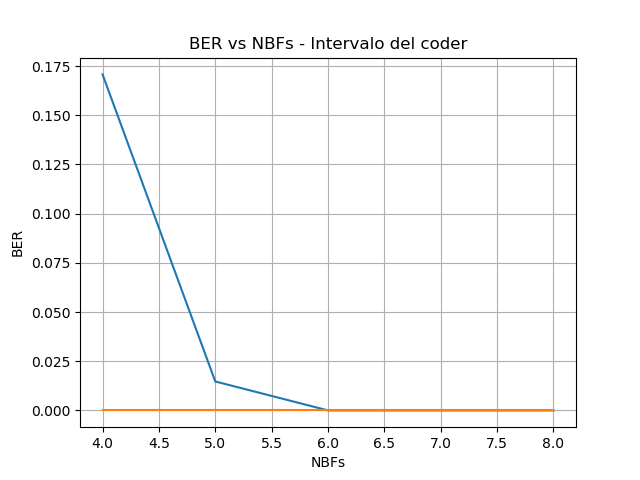
\includegraphics[width=0.60\paperwidth]{Graficos/cuantization.png}%
\end{figure}
\end{frame}

\begin{frame}{Resolución de probabilidades}
\begin{itemize}
    \item  La resolución de los intervalos del codificador se mantiene constante.
    \item  La resolución elegida para este grupo de variables será U(5,4).
    \end{itemize}
    \begin{figure}
  \centering
  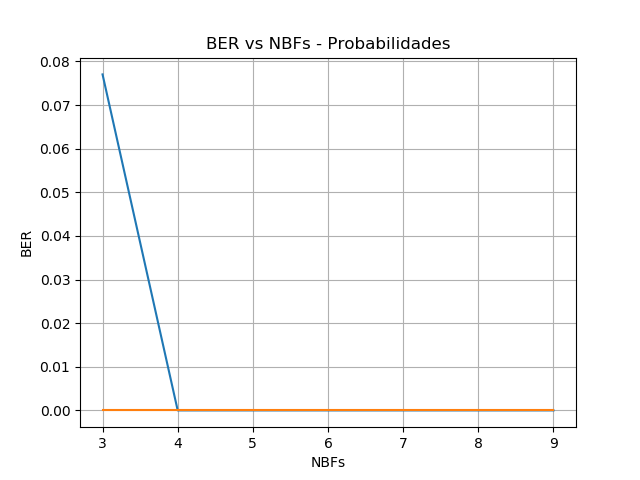
\includegraphics[width=0.60\paperwidth]{Graficos/cuantization2.png}%
\end{figure}
\end{frame}

\begin{frame}{Resolución de intervalos del decodificador}
\begin{itemize}
    \item Se mantiene constante la resolución de los intervalos del codificador y las variables de probabilidad.
    \item La resolución elegida para este grupo es U(10,9).
    \end{itemize}
    \begin{figure}
  \centering
  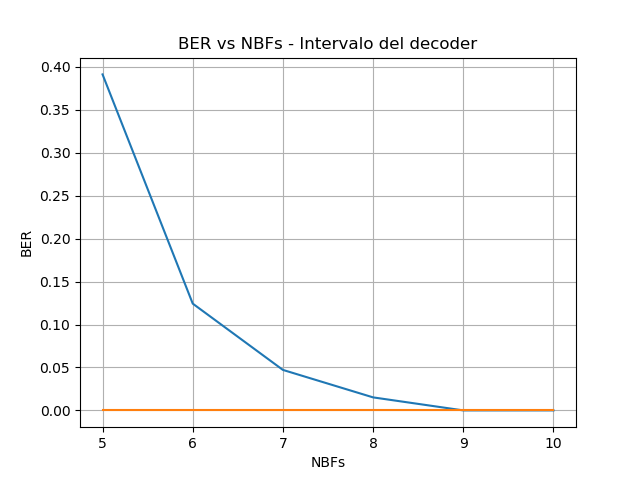
\includegraphics[width=0.60\paperwidth]{Graficos/cuantization3.png}%
\end{figure}
\end{frame}

\begin{frame}{Resoluciones sin considerar escalado}
\begin{itemize}
    \item Cuantización de intervalos del codificador 
\end{itemize}
    \begin{figure}
  \centering
  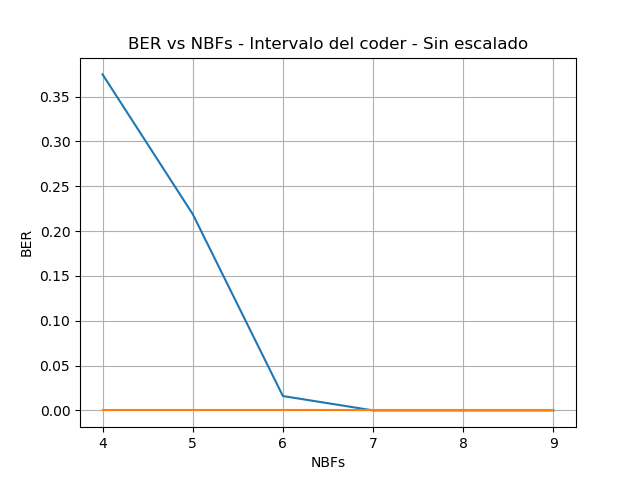
\includegraphics[width=0.60\paperwidth]{Graficos/cuantization4.png}%
\end{figure}
\end{frame}

\begin{frame}{Resoluciones sin considerar escalado}
    \begin{itemize}
        \item Cuantización de las variables de probabilidad 
    \end{itemize}
     
    \begin{figure}
  \centering
  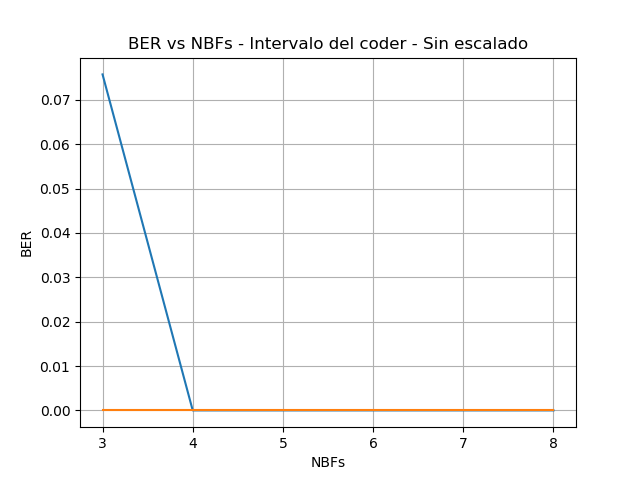
\includegraphics[width=0.60\paperwidth]{Graficos/cuantization5.png}%
\end{figure}
\end{frame}

\begin{frame}{Resoluciones sin considerar escalado}
    \begin{itemize}
        \item Cuantización de intervalos del decodificador 
    \end{itemize}
    \begin{figure}
  \centering
  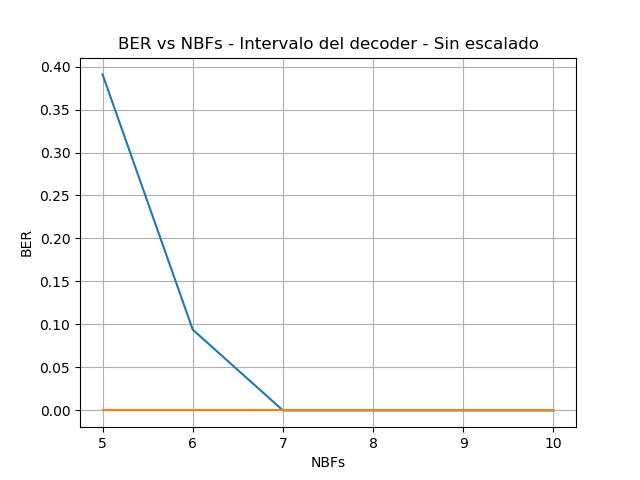
\includegraphics[width=0.60\paperwidth]{Graficos/cuantization6.png}%
\end{figure}
\end{frame}

\begin{frame}{Resoluciones con y sin  escalado}
 \begin{itemize}
     \item Con escalado:
        \begin{itemize}
        \item Intervalo del codificador: U(7,6)
         \item Probabilidades: U(5,4)
        \item Intervalo del decodificador: U(10,9)
        \end{itemize}

     \item  Sin escalado:
        \begin{itemize}
        \item Intervalo del codificador: U(8,7)
         \item Probabilidades: U(5,4)
        \item Intervalo del decodificador: U(8,7)
        \end{itemize}
 \end{itemize}
\end{frame}

\begin{frame}{Retardos en la salida del codificador}
 \begin{itemize}
     \item Se deben incluir de tal forma que no afecte el sincronismo de datos
      \item Se agregó una cantidad de retardos en el canal de comunicación para que esto no sea un problema

    \item Por ejemplo:\\
    La secuencia [1,0,0,0] se codifica a [0,1,0,0,0,0,1,0], si el canal presenta un retardo, la secuencia será [1,0,0,0,1,0,0,0]
     \end{itemize}
\end{frame}

\subsection{Implementación}

\begin{frame}{Bloque codificador}
    \begin{figure}
  \centering
  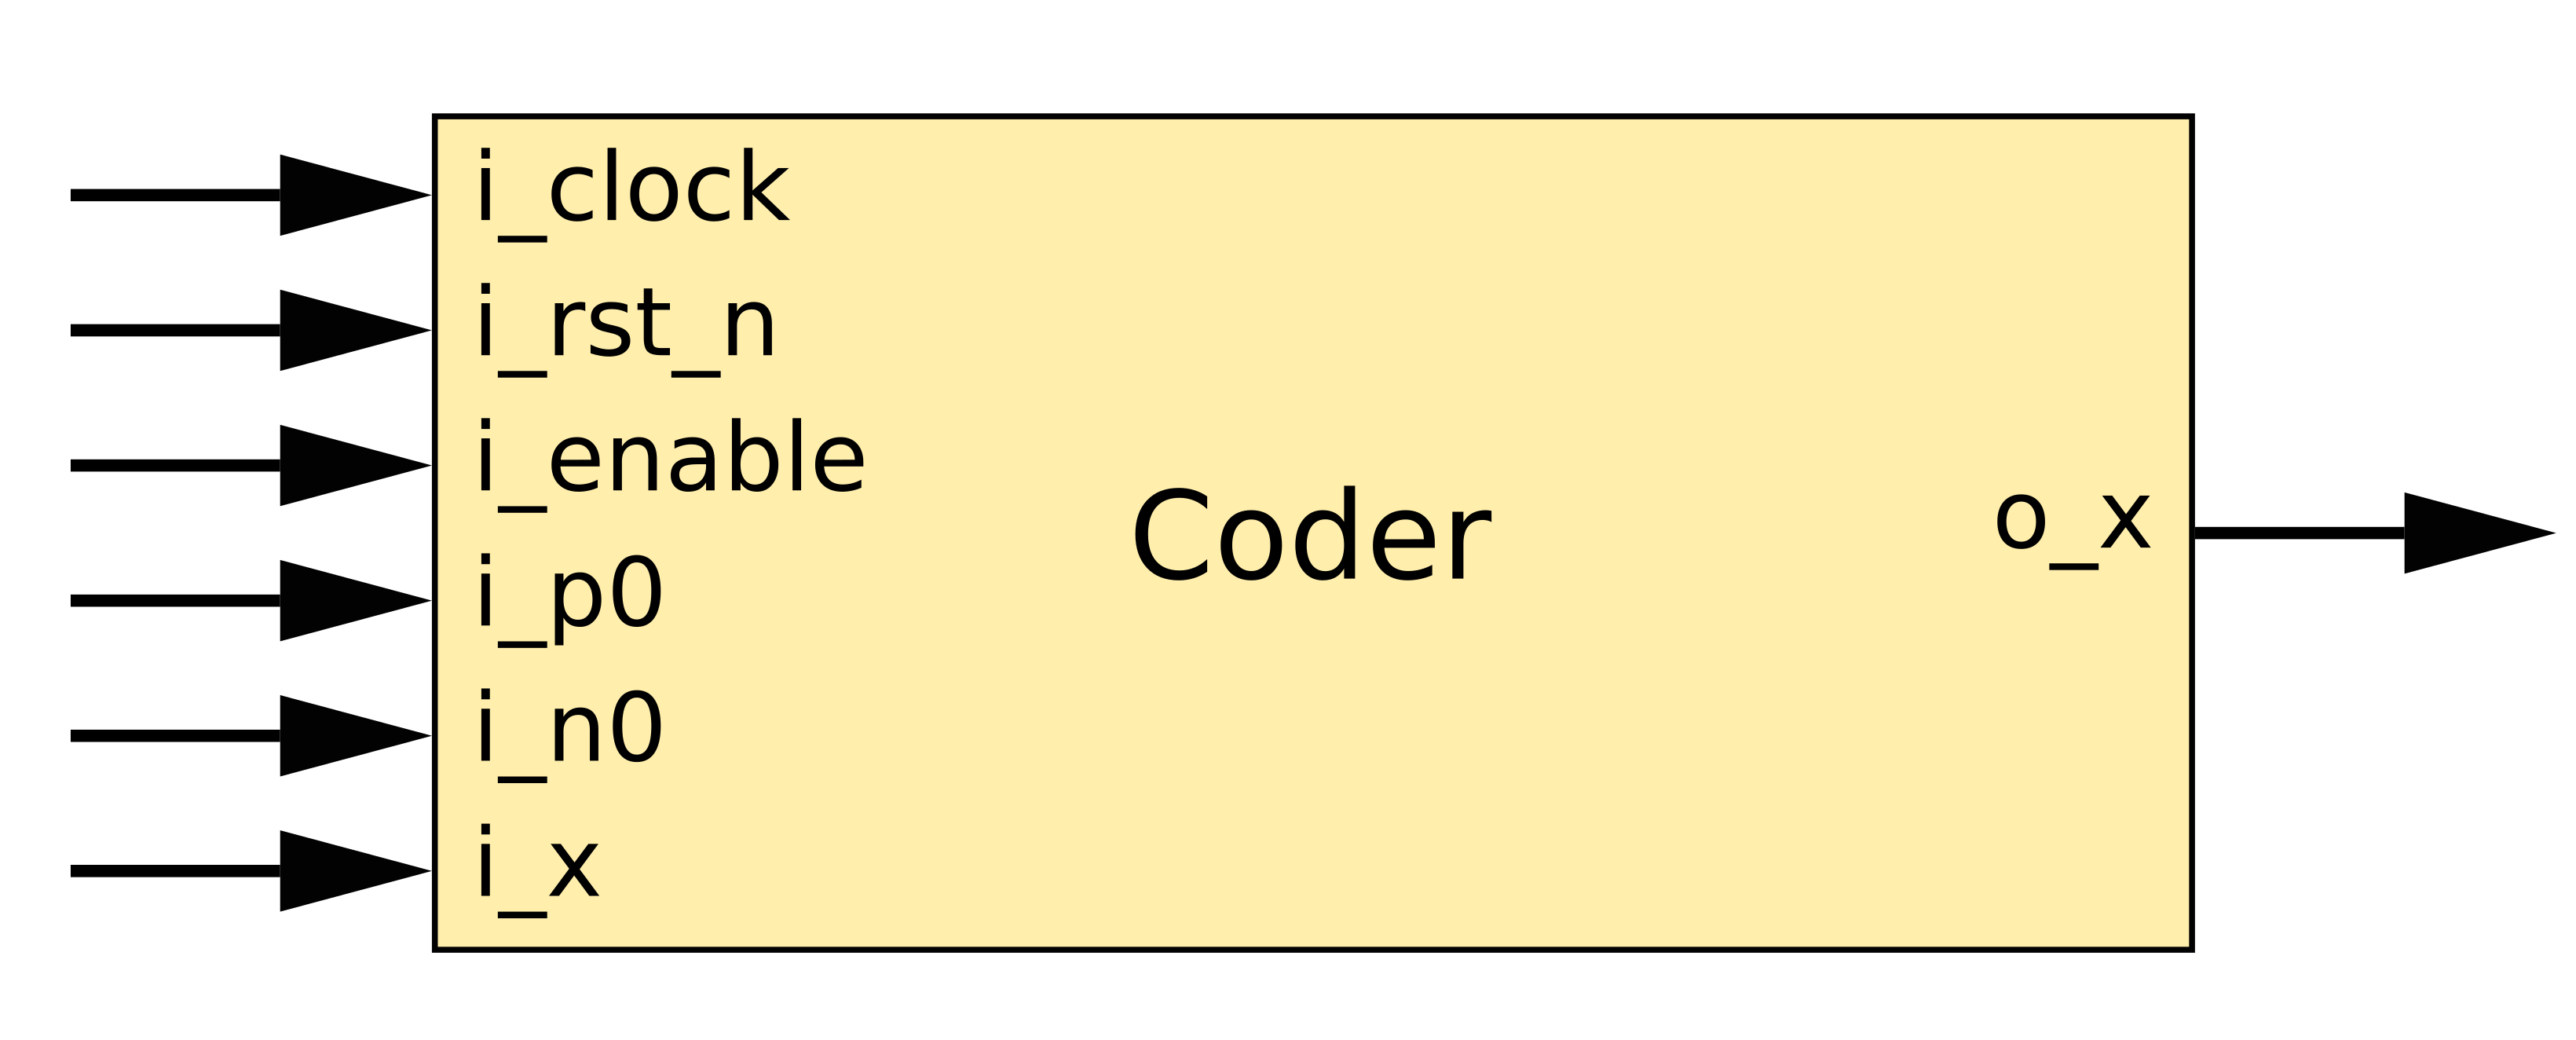
\includegraphics[width=0.70\paperwidth]{Diagramas/coder.png}%
\end{figure}
\end{frame}

\begin{frame}{Bloque codificador, estructura interna}
    
 \begin{figure}
  \centering
  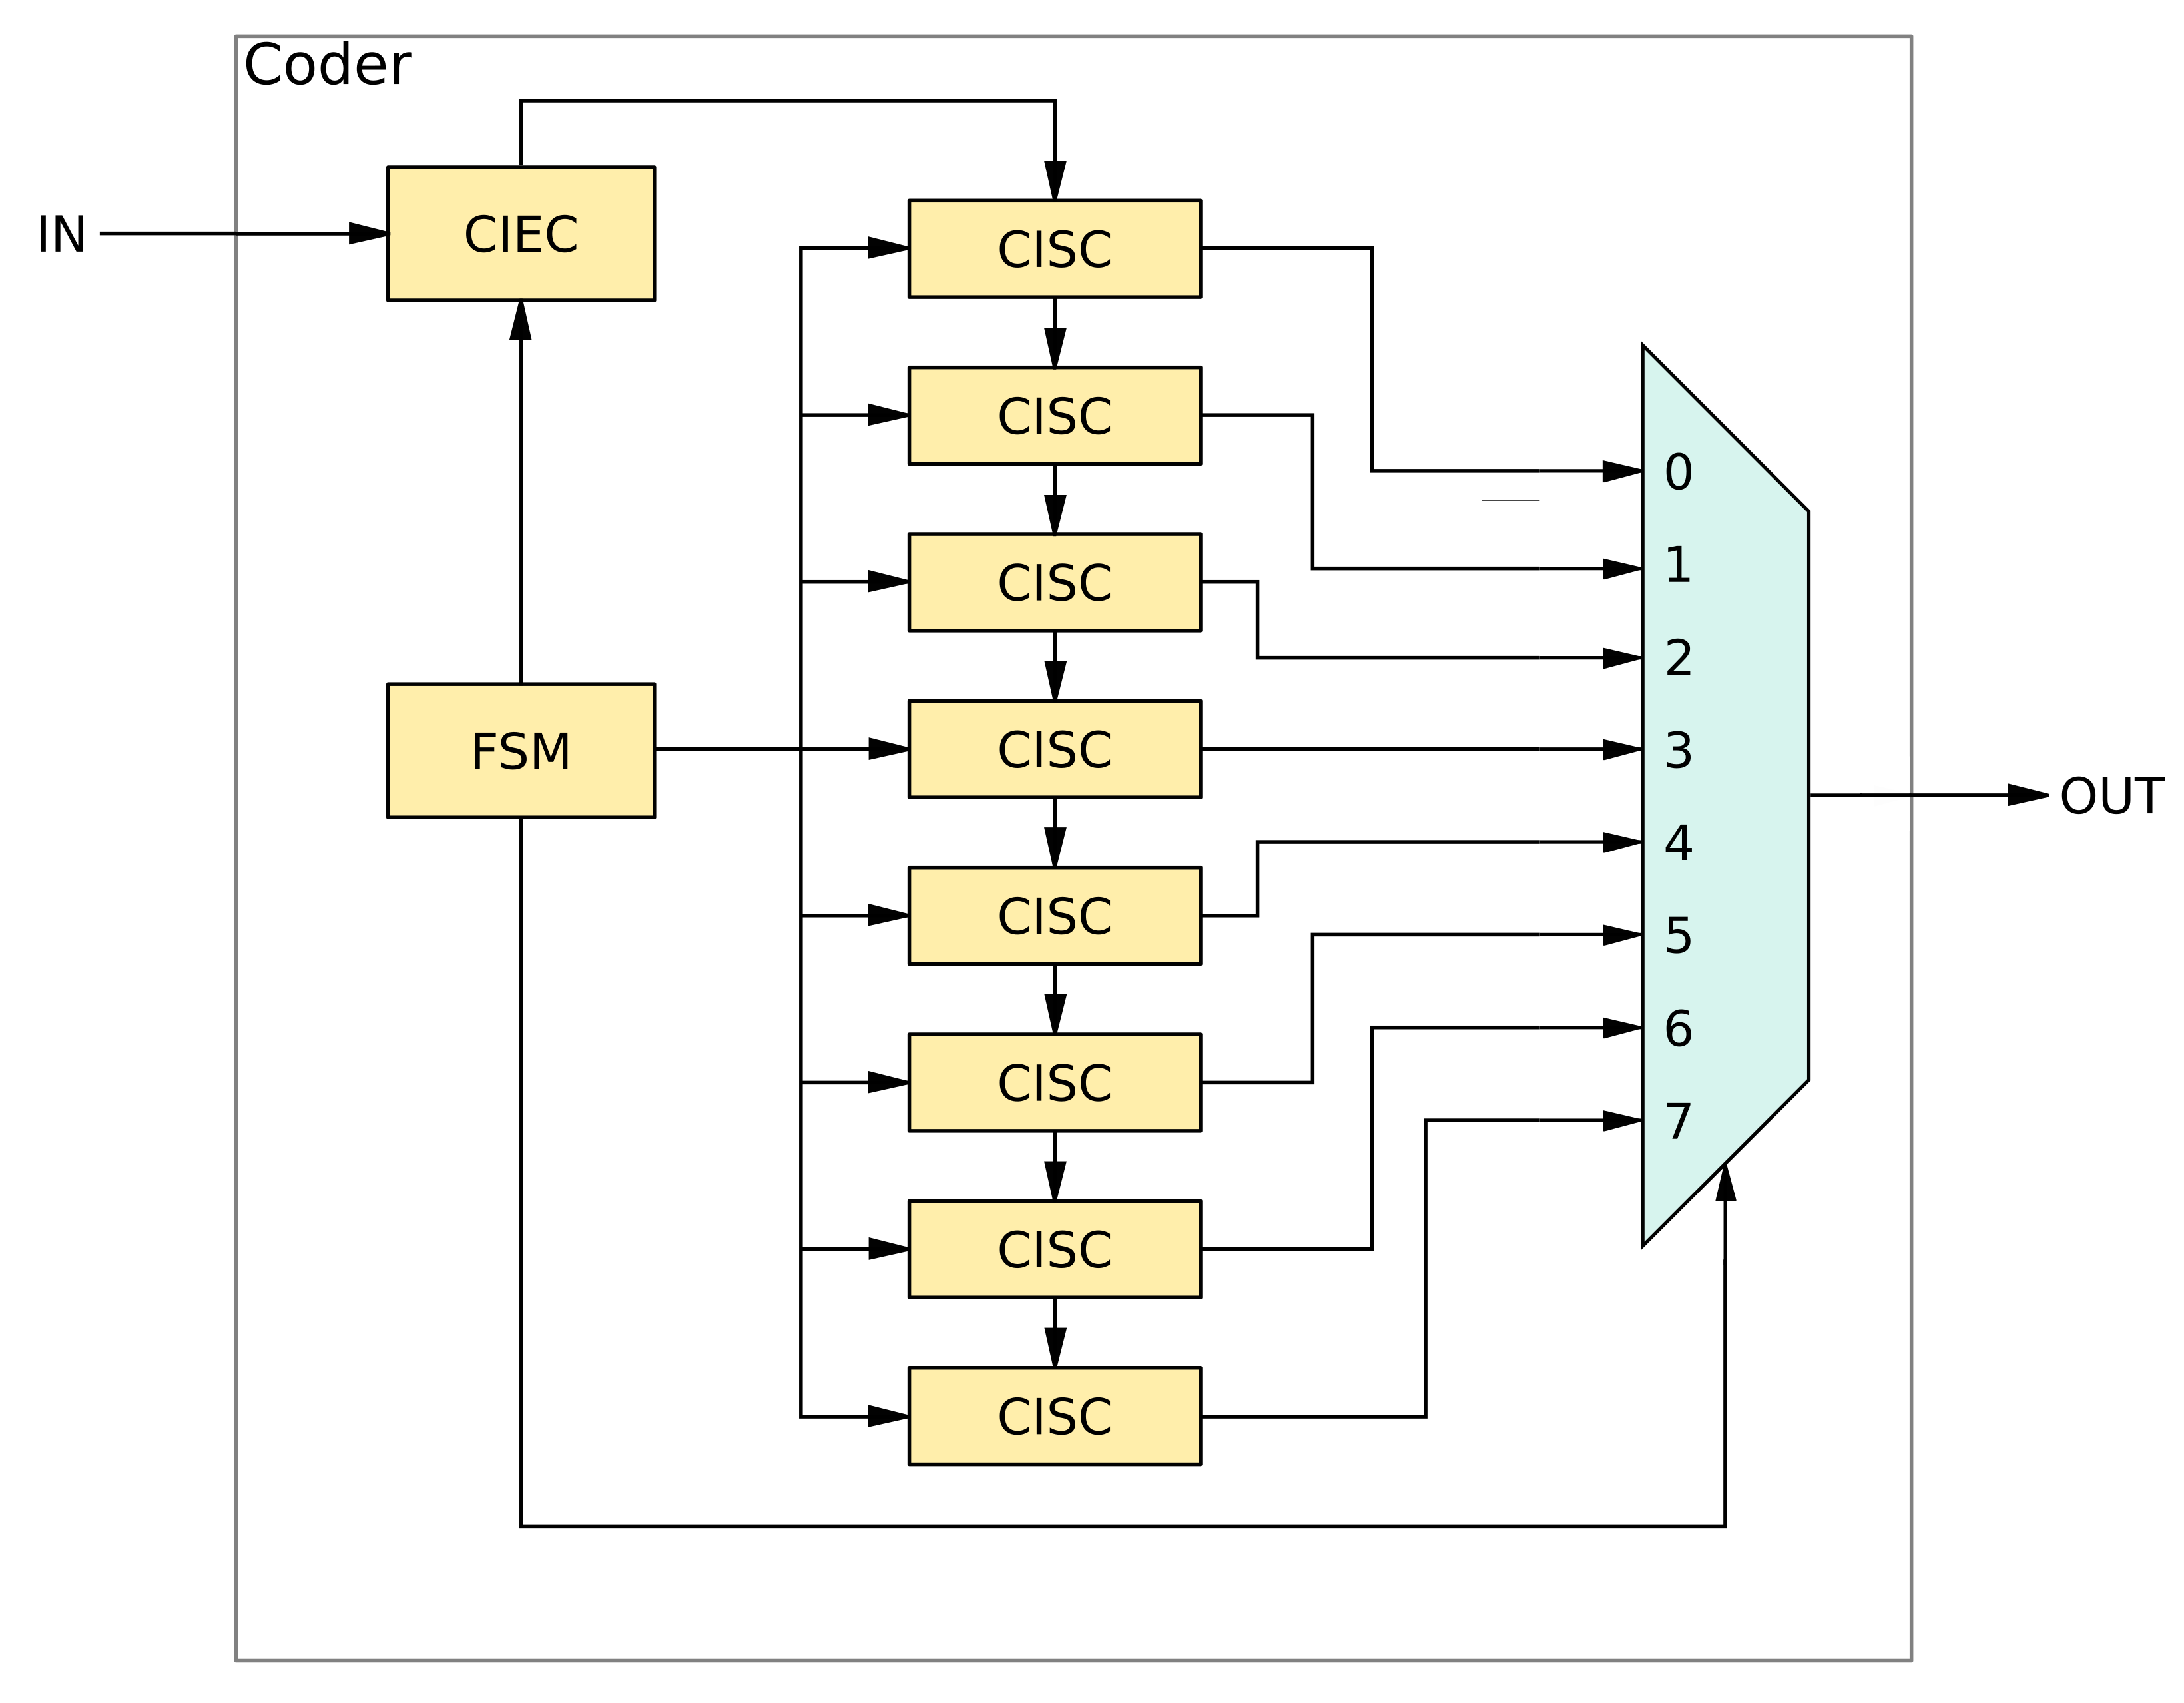
\includegraphics[width=0.70\paperwidth]{Diagramas/internal_coder.png}%
\end{figure}
\end{frame}

\begin{frame}{Bloque codificador}
\begin{enumerate}
    \item Cuando el bloque CIEC\footnote{Calculo de Intervalo de Entrada de Coder} finaliza se activa el primer bloque CISC\footnote{Calculo de Intervalo de Salida de Coder} 
    \item  La FSM deshabilita el primer bloque CISC actual y activa el siguiente.
    \item Se selecciona la salida del bloque CISC actual
    \item Este proceso se repite con todos los bloques CISC
\end{enumerate}
\end{frame}


\begin{frame}{Bloque CIEC}
 \begin{figure}
  \centering
  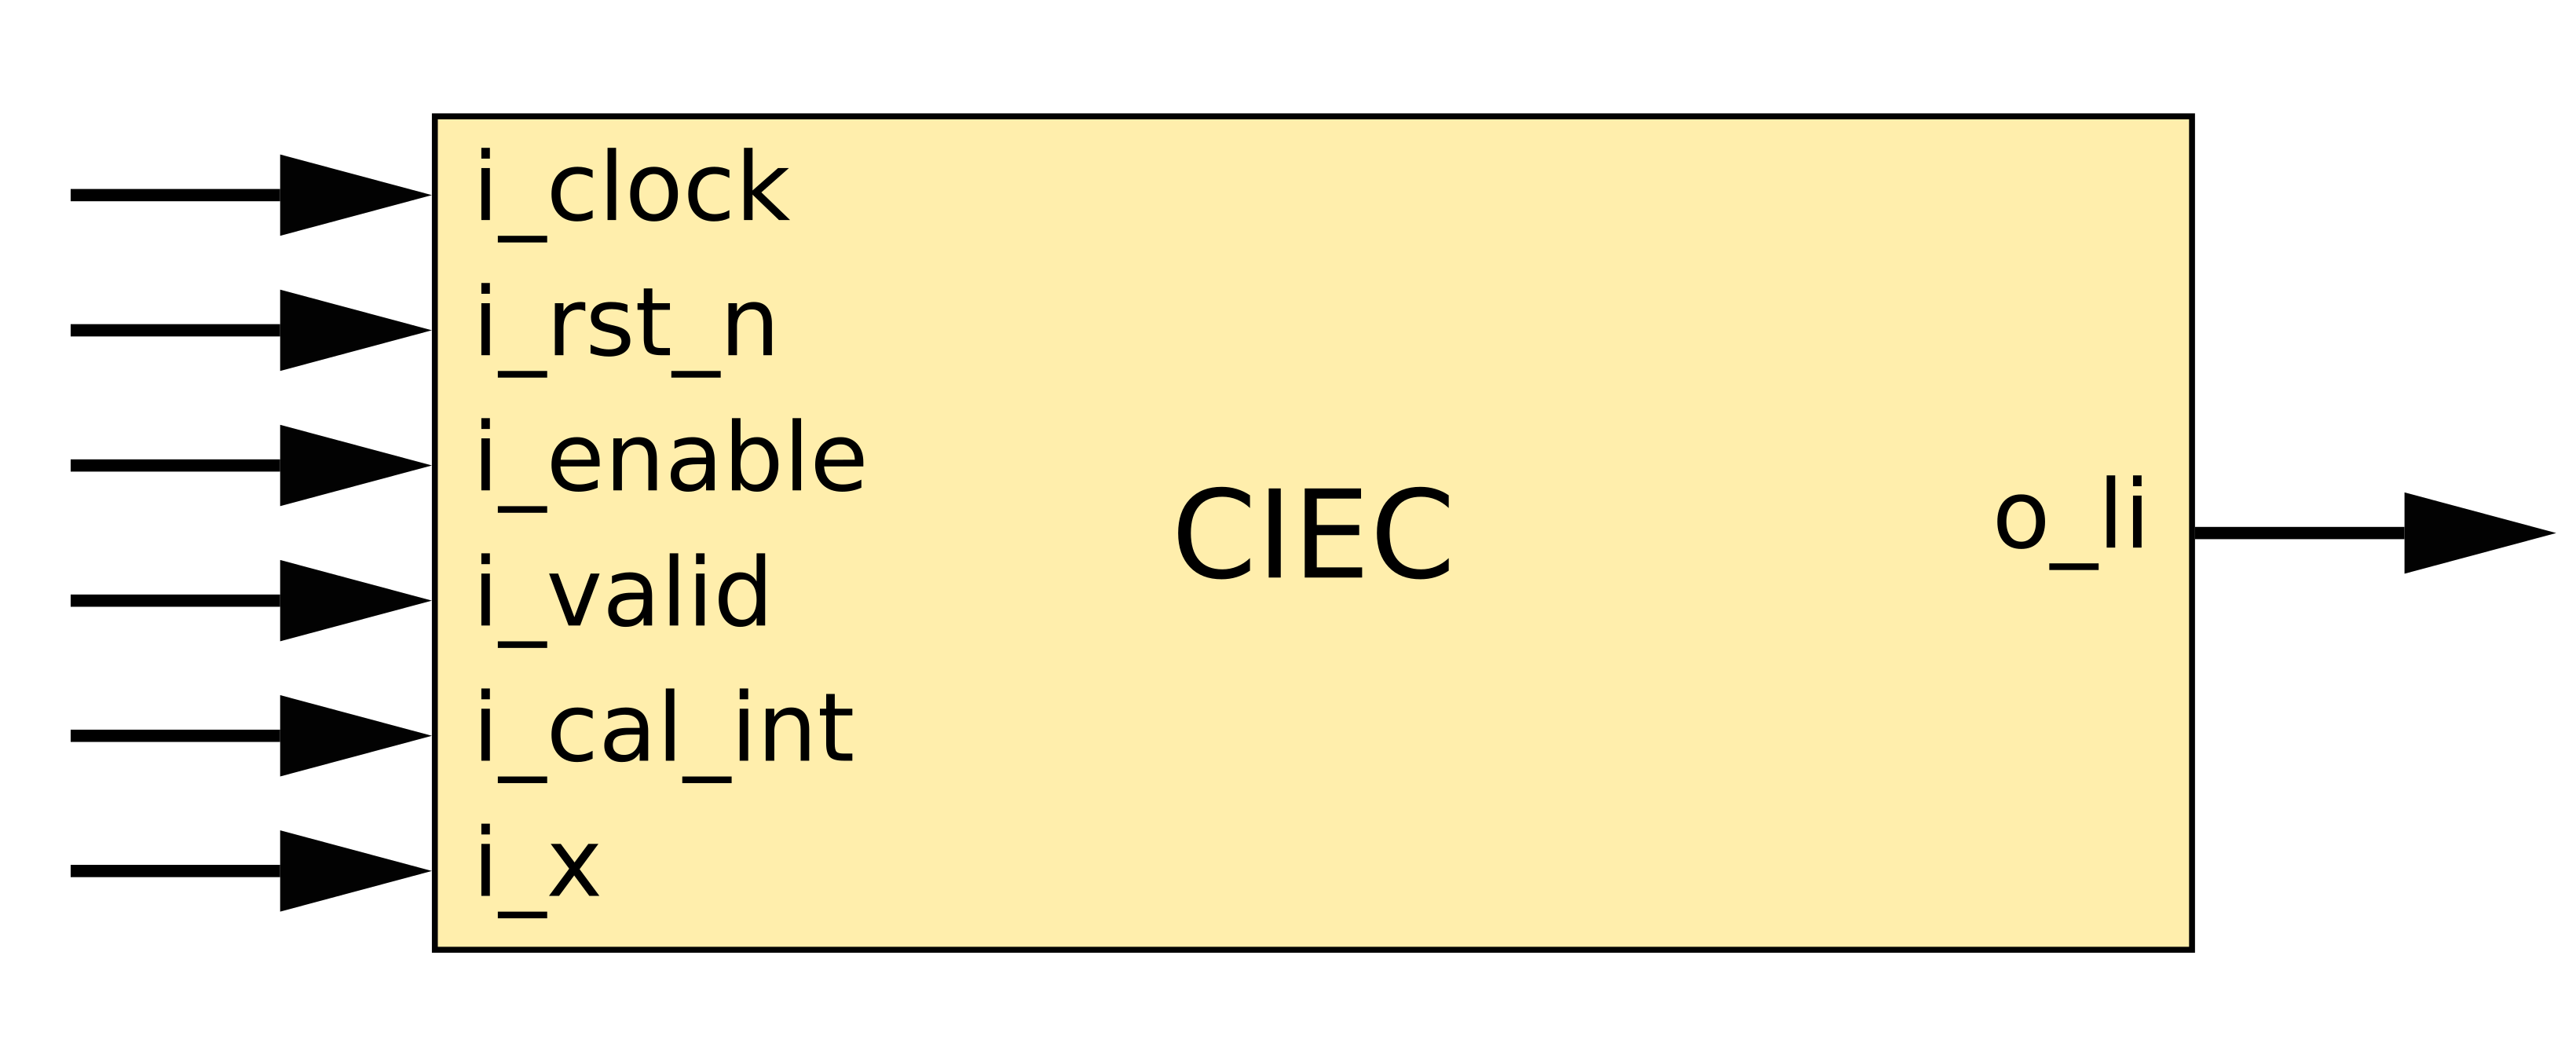
\includegraphics[width=0.70\paperwidth]{Diagramas/ciec.png}%
\end{figure}
\end{frame}

\begin{frame}{CIEC, estructura interna}

 \begin{figure}
  \centering
  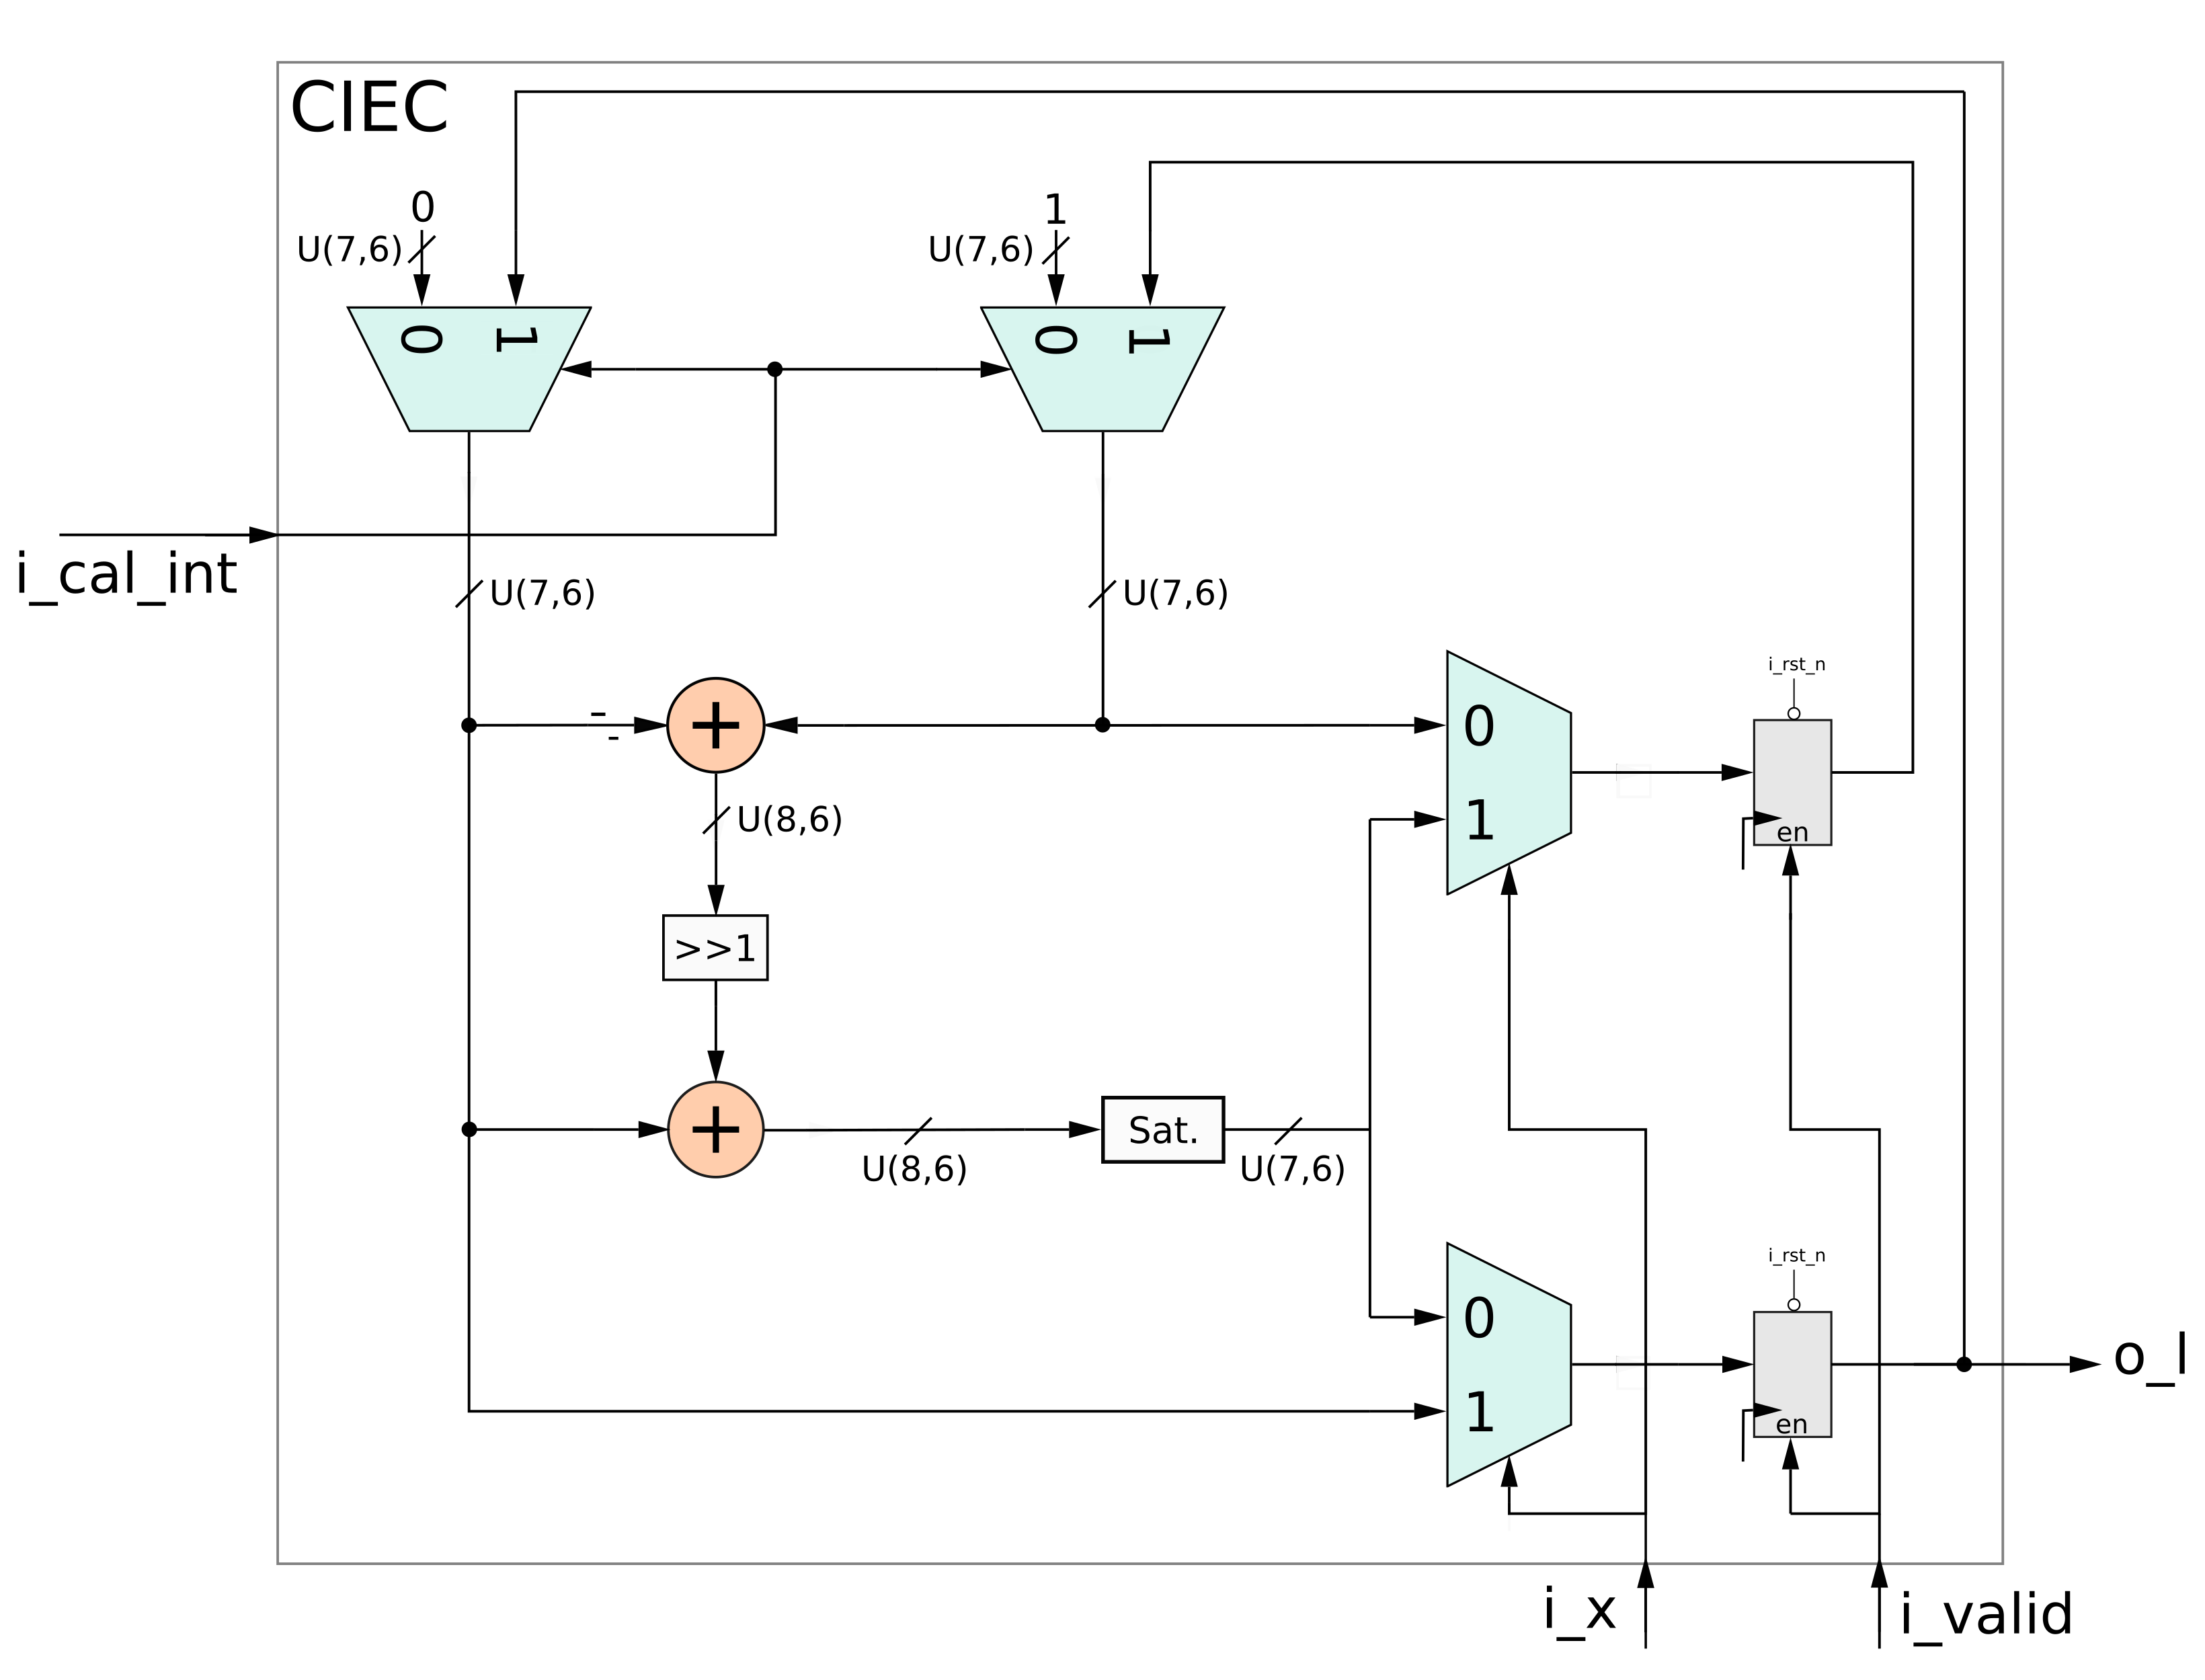
\includegraphics[width=0.70\paperwidth]{Diagramas/internal_ciec.png}%
\end{figure}
\end{frame}

\begin{frame}{Bloque CISC}

 \begin{figure}
  \centering
  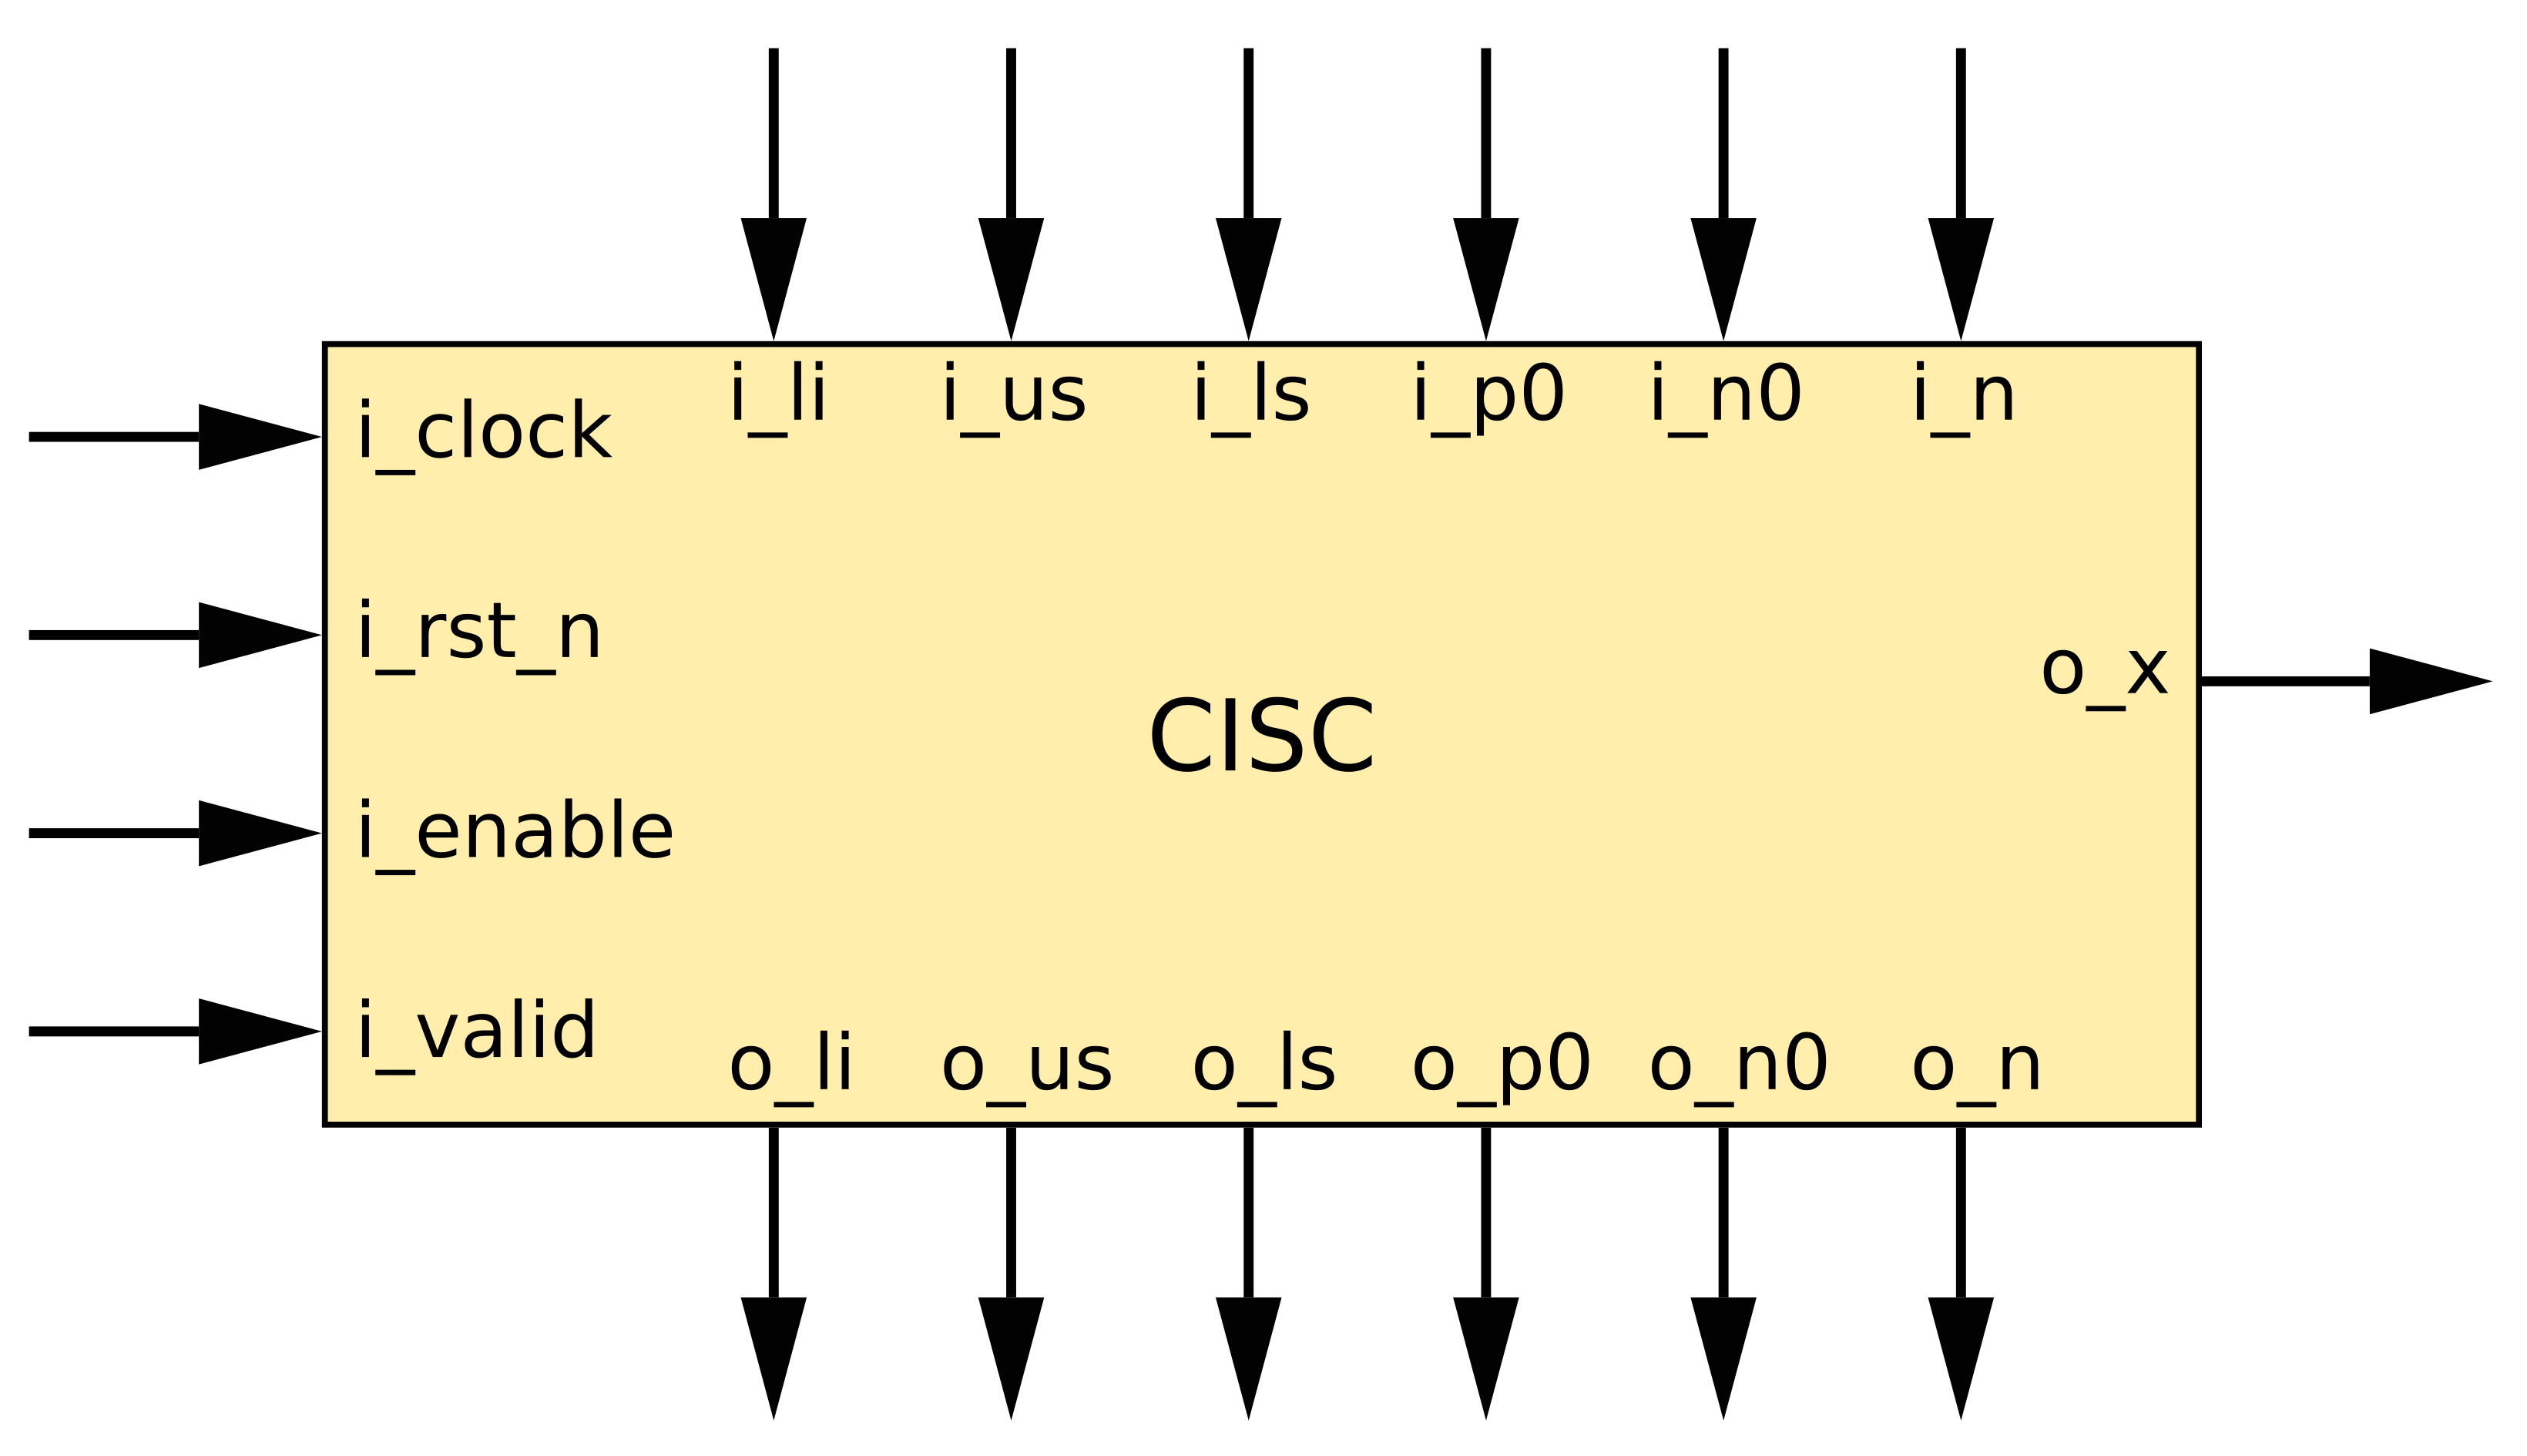
\includegraphics[width=0.70\paperwidth]{Diagramas/cisc.png}%
\end{figure}
\end{frame}

\begin{frame}{CISC, estructura interna}

 \begin{figure}
  \centering
  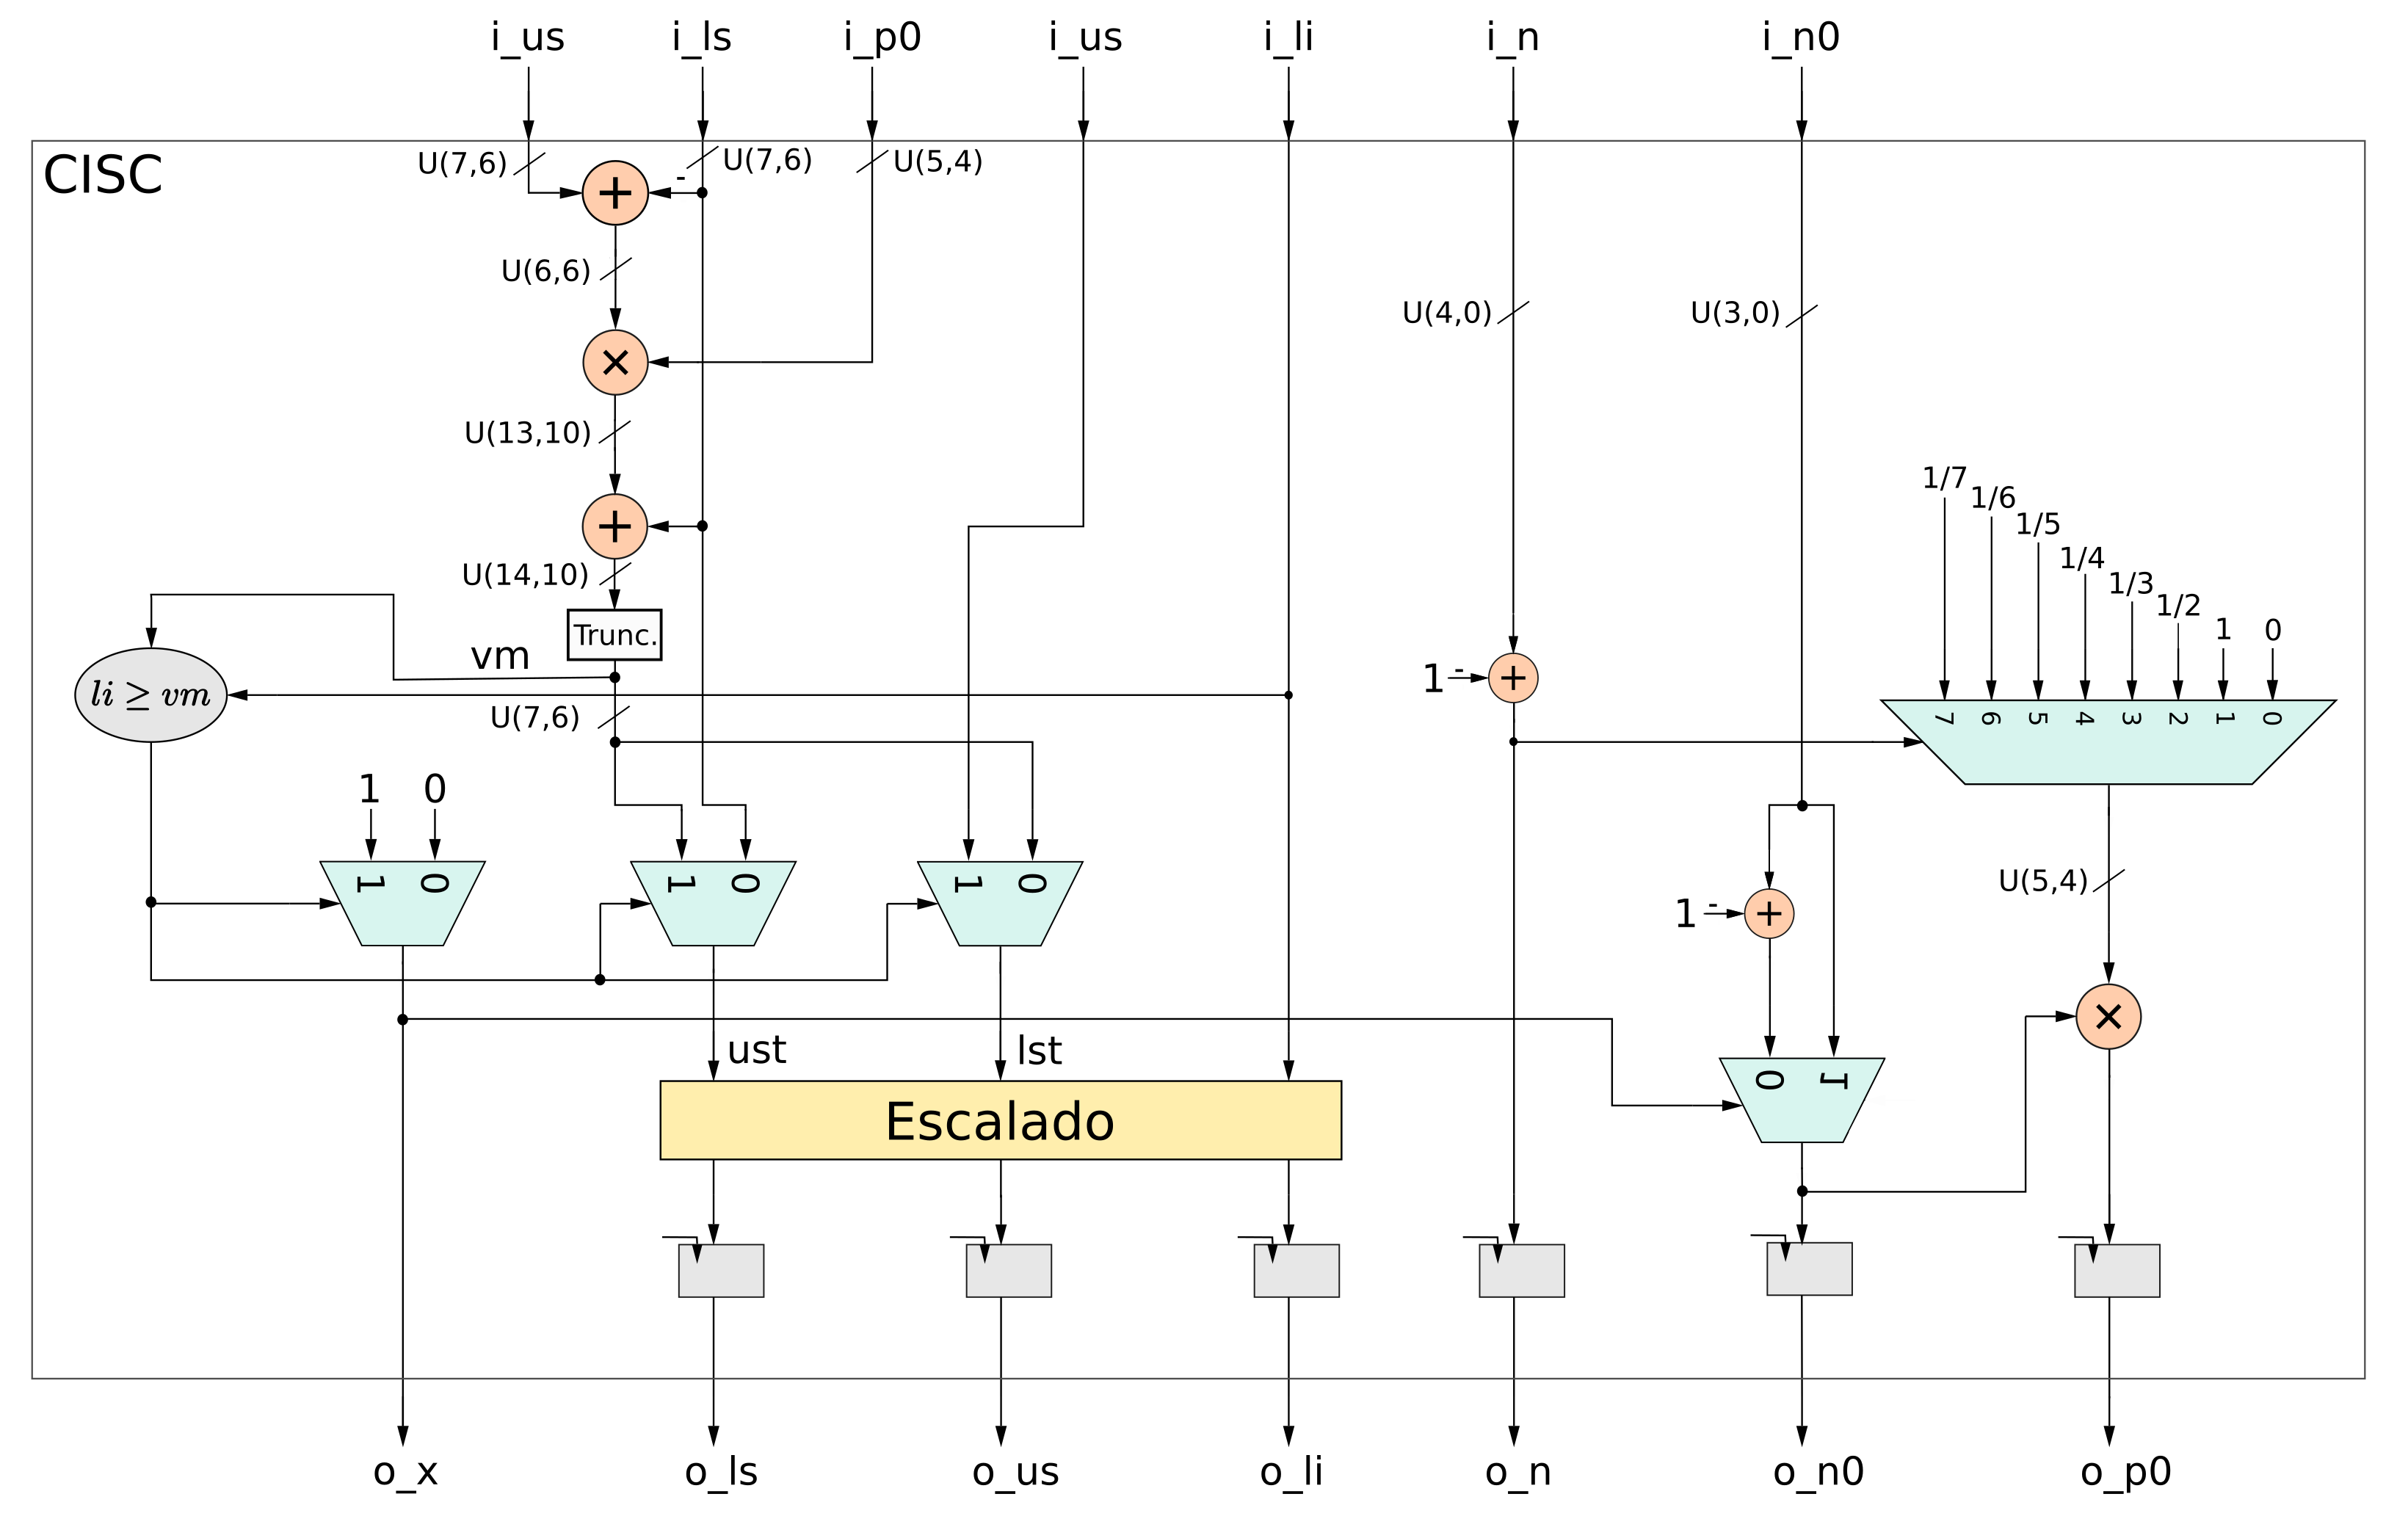
\includegraphics[width=0.70\paperwidth]{Diagramas/internal_cisc.png}%
\end{figure}
\end{frame}


\begin{frame}{Escalado, estructura interna}
 \begin{figure}
  \centering
  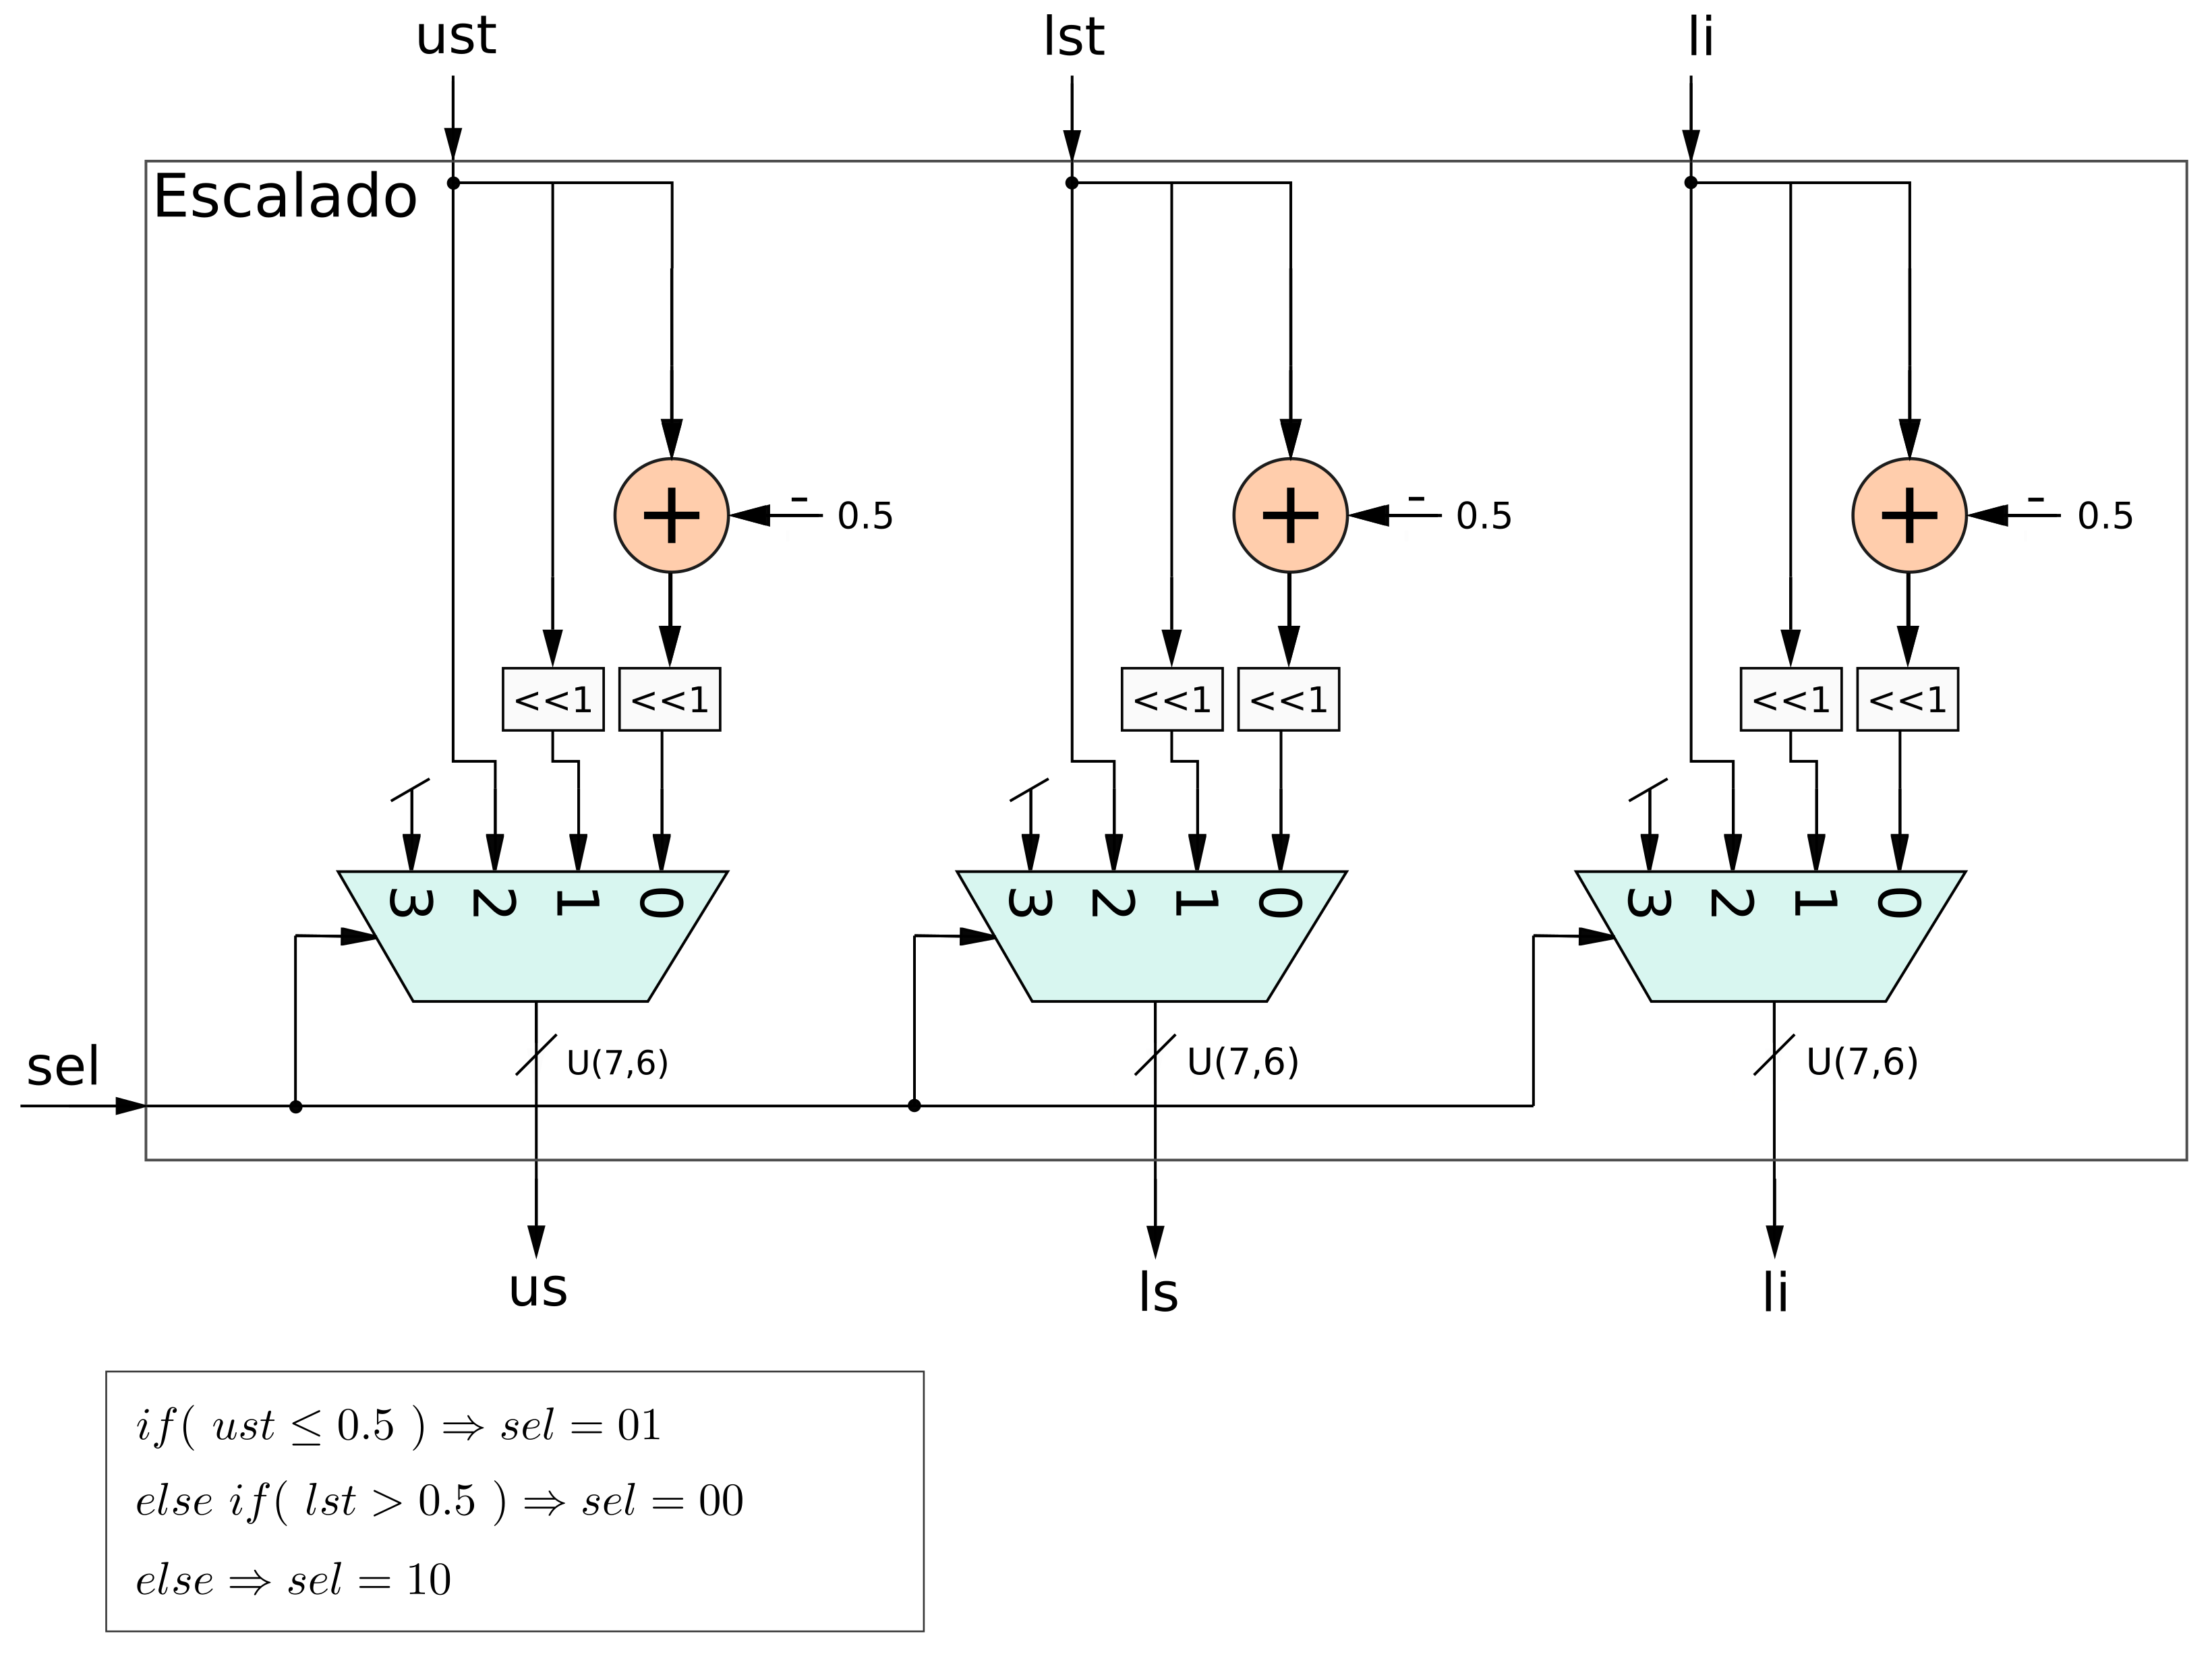
\includegraphics[width=0.70\paperwidth]{Diagramas/escalado.png}%
\end{figure}
\end{frame}

\begin{frame}{Flujo de datos de codificador}
    \begin{itemize}
        \item El bloque CIEC requiere de 4 u.t. pero es habilitado por la FSM la mitad de los ciclos, por lo que requiere 8 u.t.
        \item Se ejecuta un bloque CISC cada ciclo, por lo que requiere 8 u.t.
        \item Esto implica que se generan 8 bits de salida cada 16 unidades de tiempo
    \end{itemize}
 \begin{figure}
  \centering
  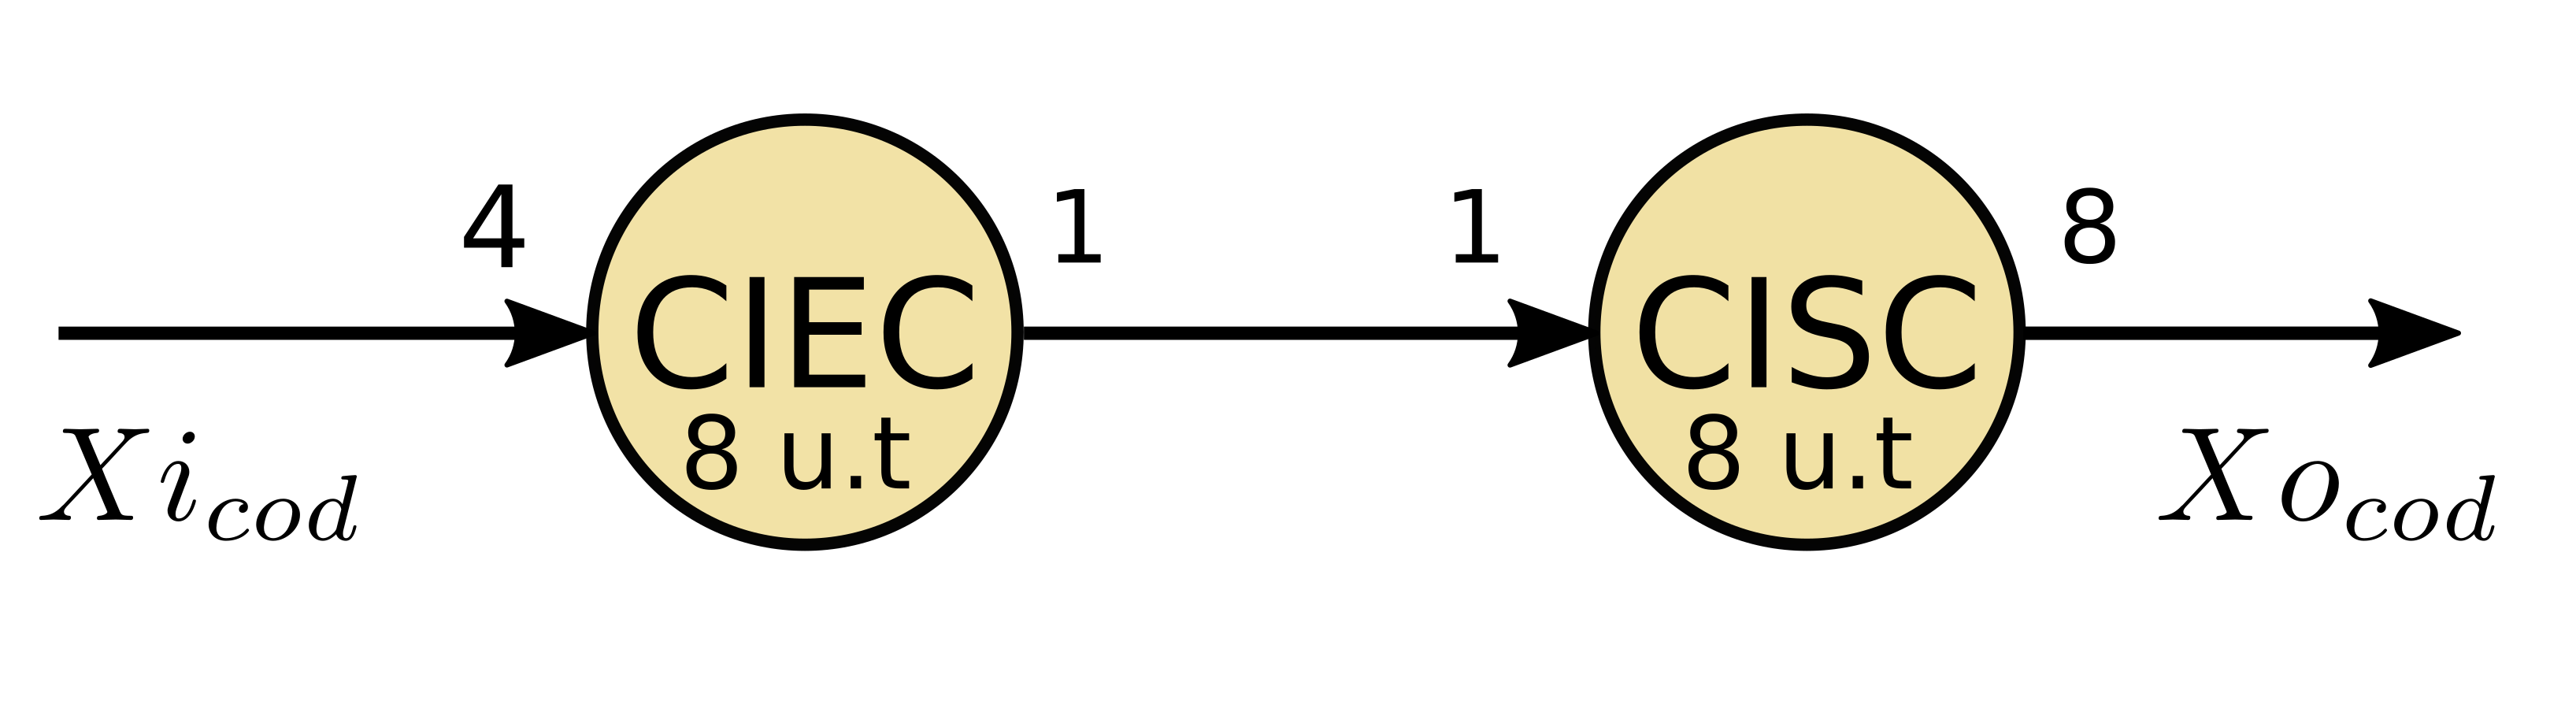
\includegraphics[width=0.70\paperwidth]{Diagramas/grafo_cod.png}%
\end{figure}
\end{frame}

\begin{frame}{Bloque decodificador}
    \begin{figure}
  \centering
  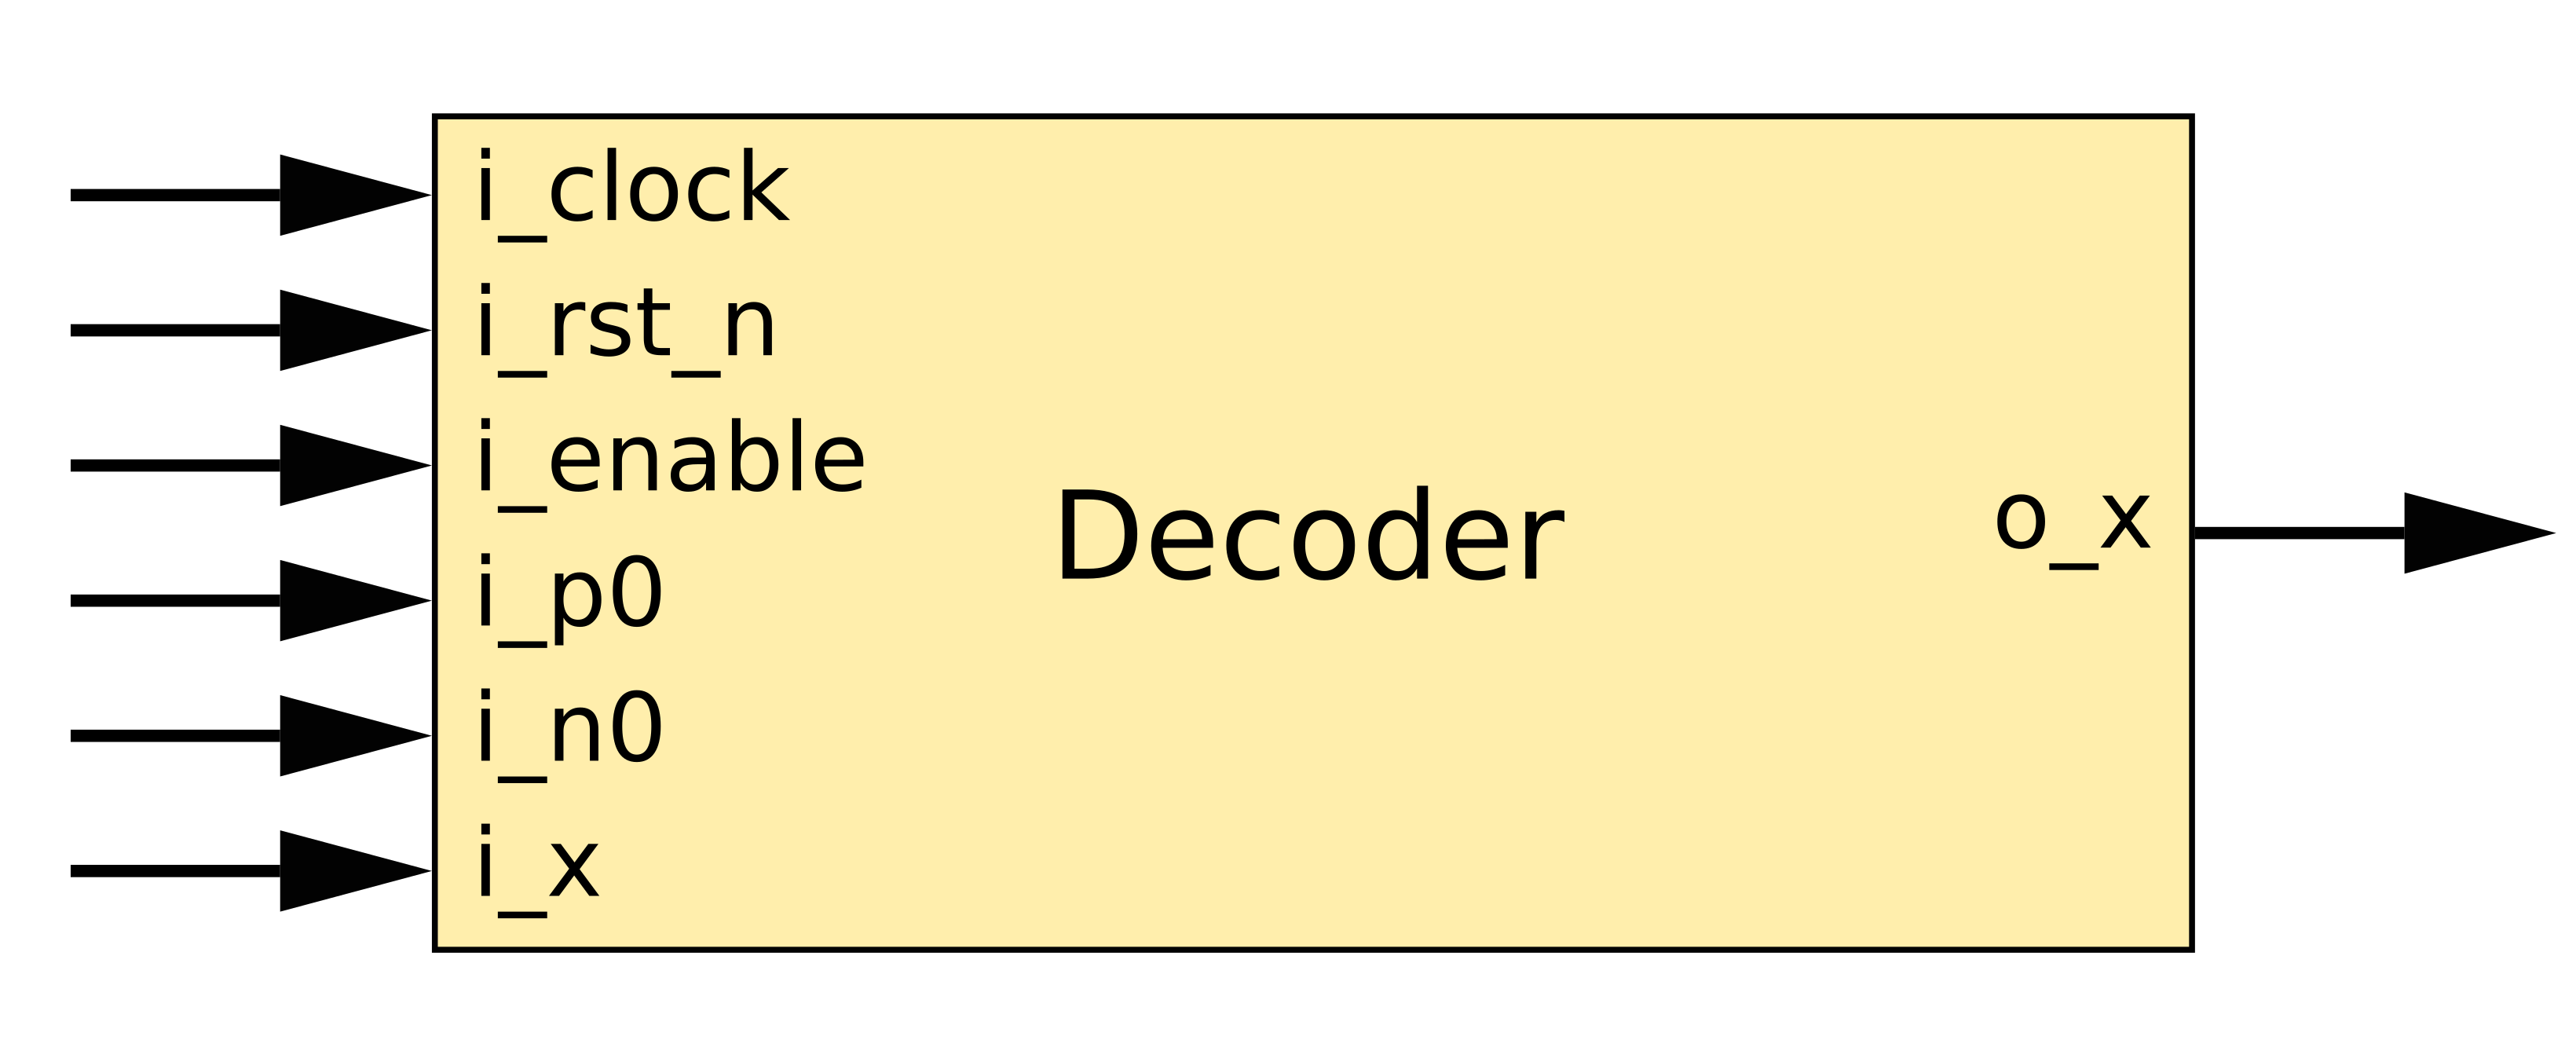
\includegraphics[width=0.70\paperwidth]{Diagramas/decoder.png}%
\end{figure}
\end{frame}

\begin{frame}{Bloque decodificador, estructura interna}
 
 \begin{itemize}
    \item  El proceso de CIED\footnote{Cálculo de Intervalo de Entrada de Decoder} y CISD\footnote{Cálculo de Intervalo de Salida de Decoder} se realiza mediante bloques recursivos
    \item La FSM habilita el bloque CISD la mitad de los ciclos de reloj con respecto al CIED
\end{itemize}
 
 \begin{figure}
  \centering
  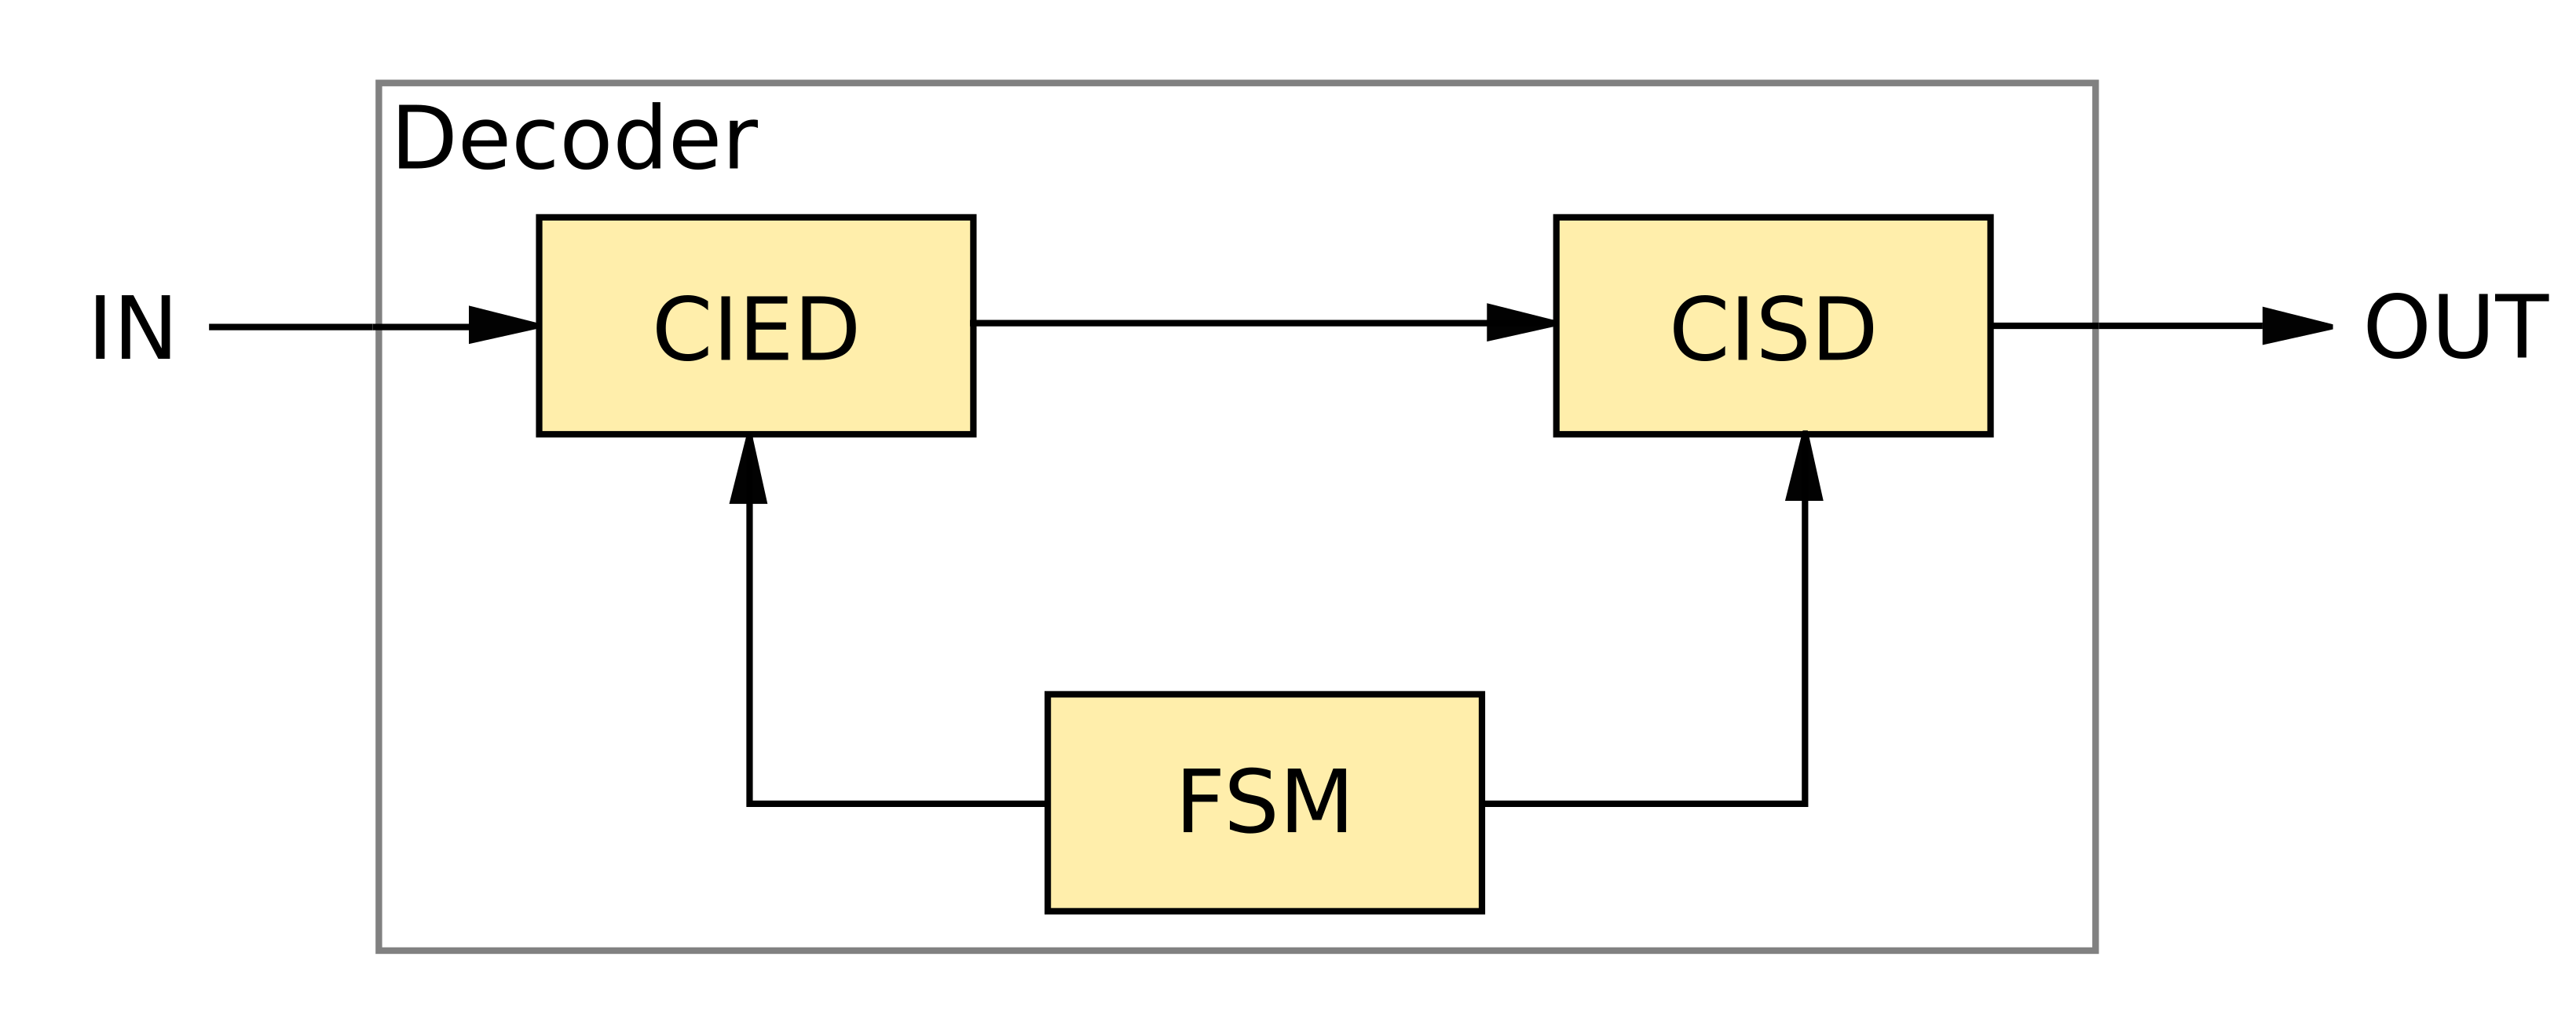
\includegraphics[width=0.70\paperwidth]{Diagramas/internal_decoder.png}%
\end{figure}
\end{frame}





\begin{frame}{Bloque CIED}

 \begin{figure}
  \centering
  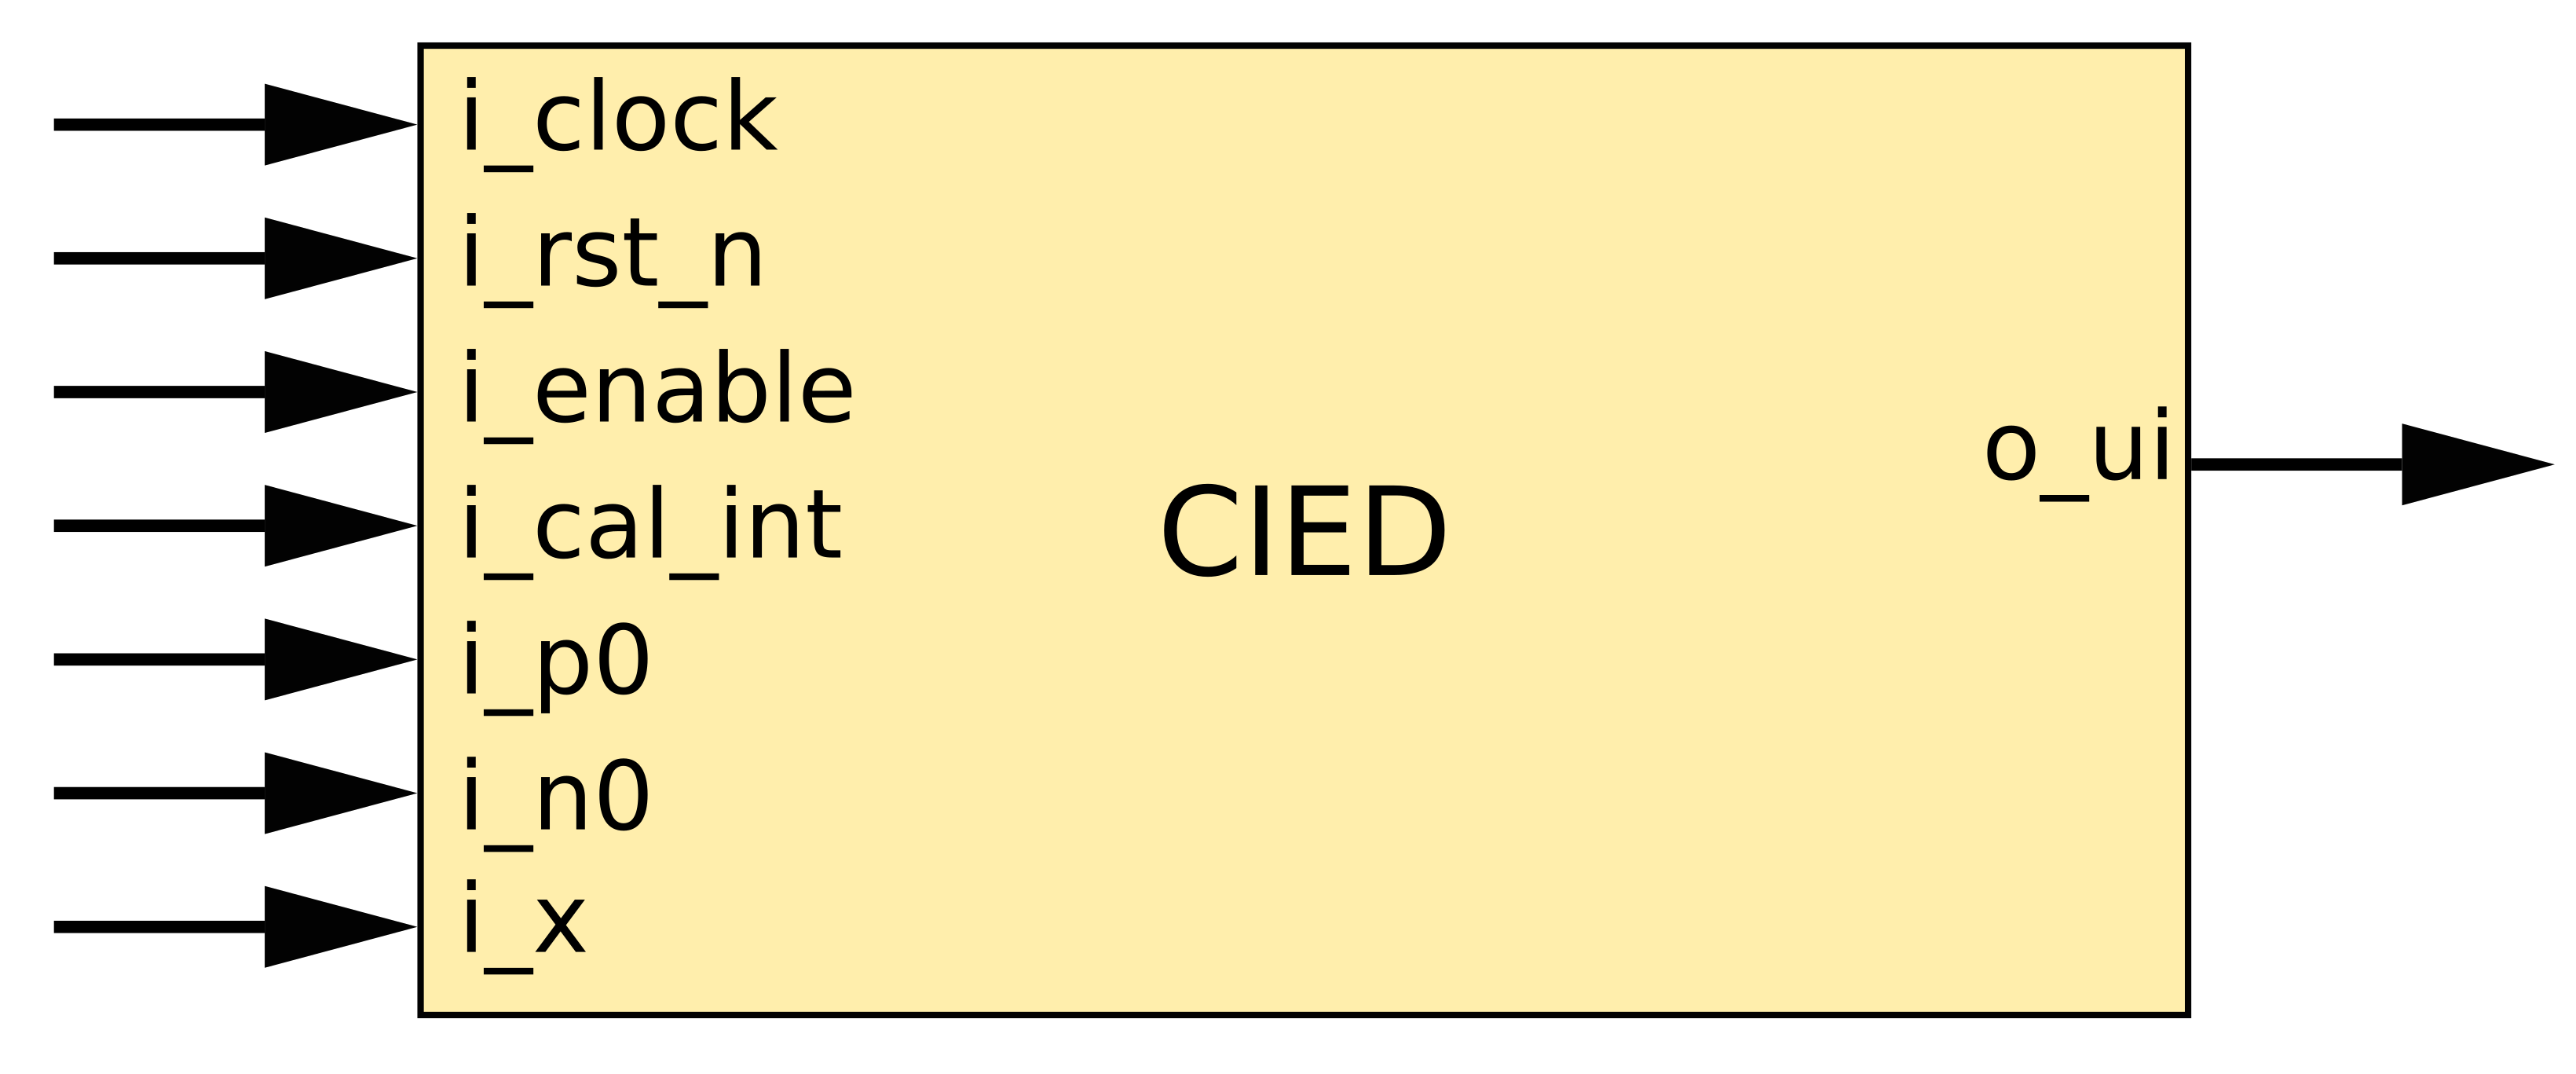
\includegraphics[width=0.70\paperwidth]{Diagramas/cied.png}%
\end{figure}
\end{frame}

\begin{frame}{CIED, estructura interna}

 \begin{figure}
  \centering
  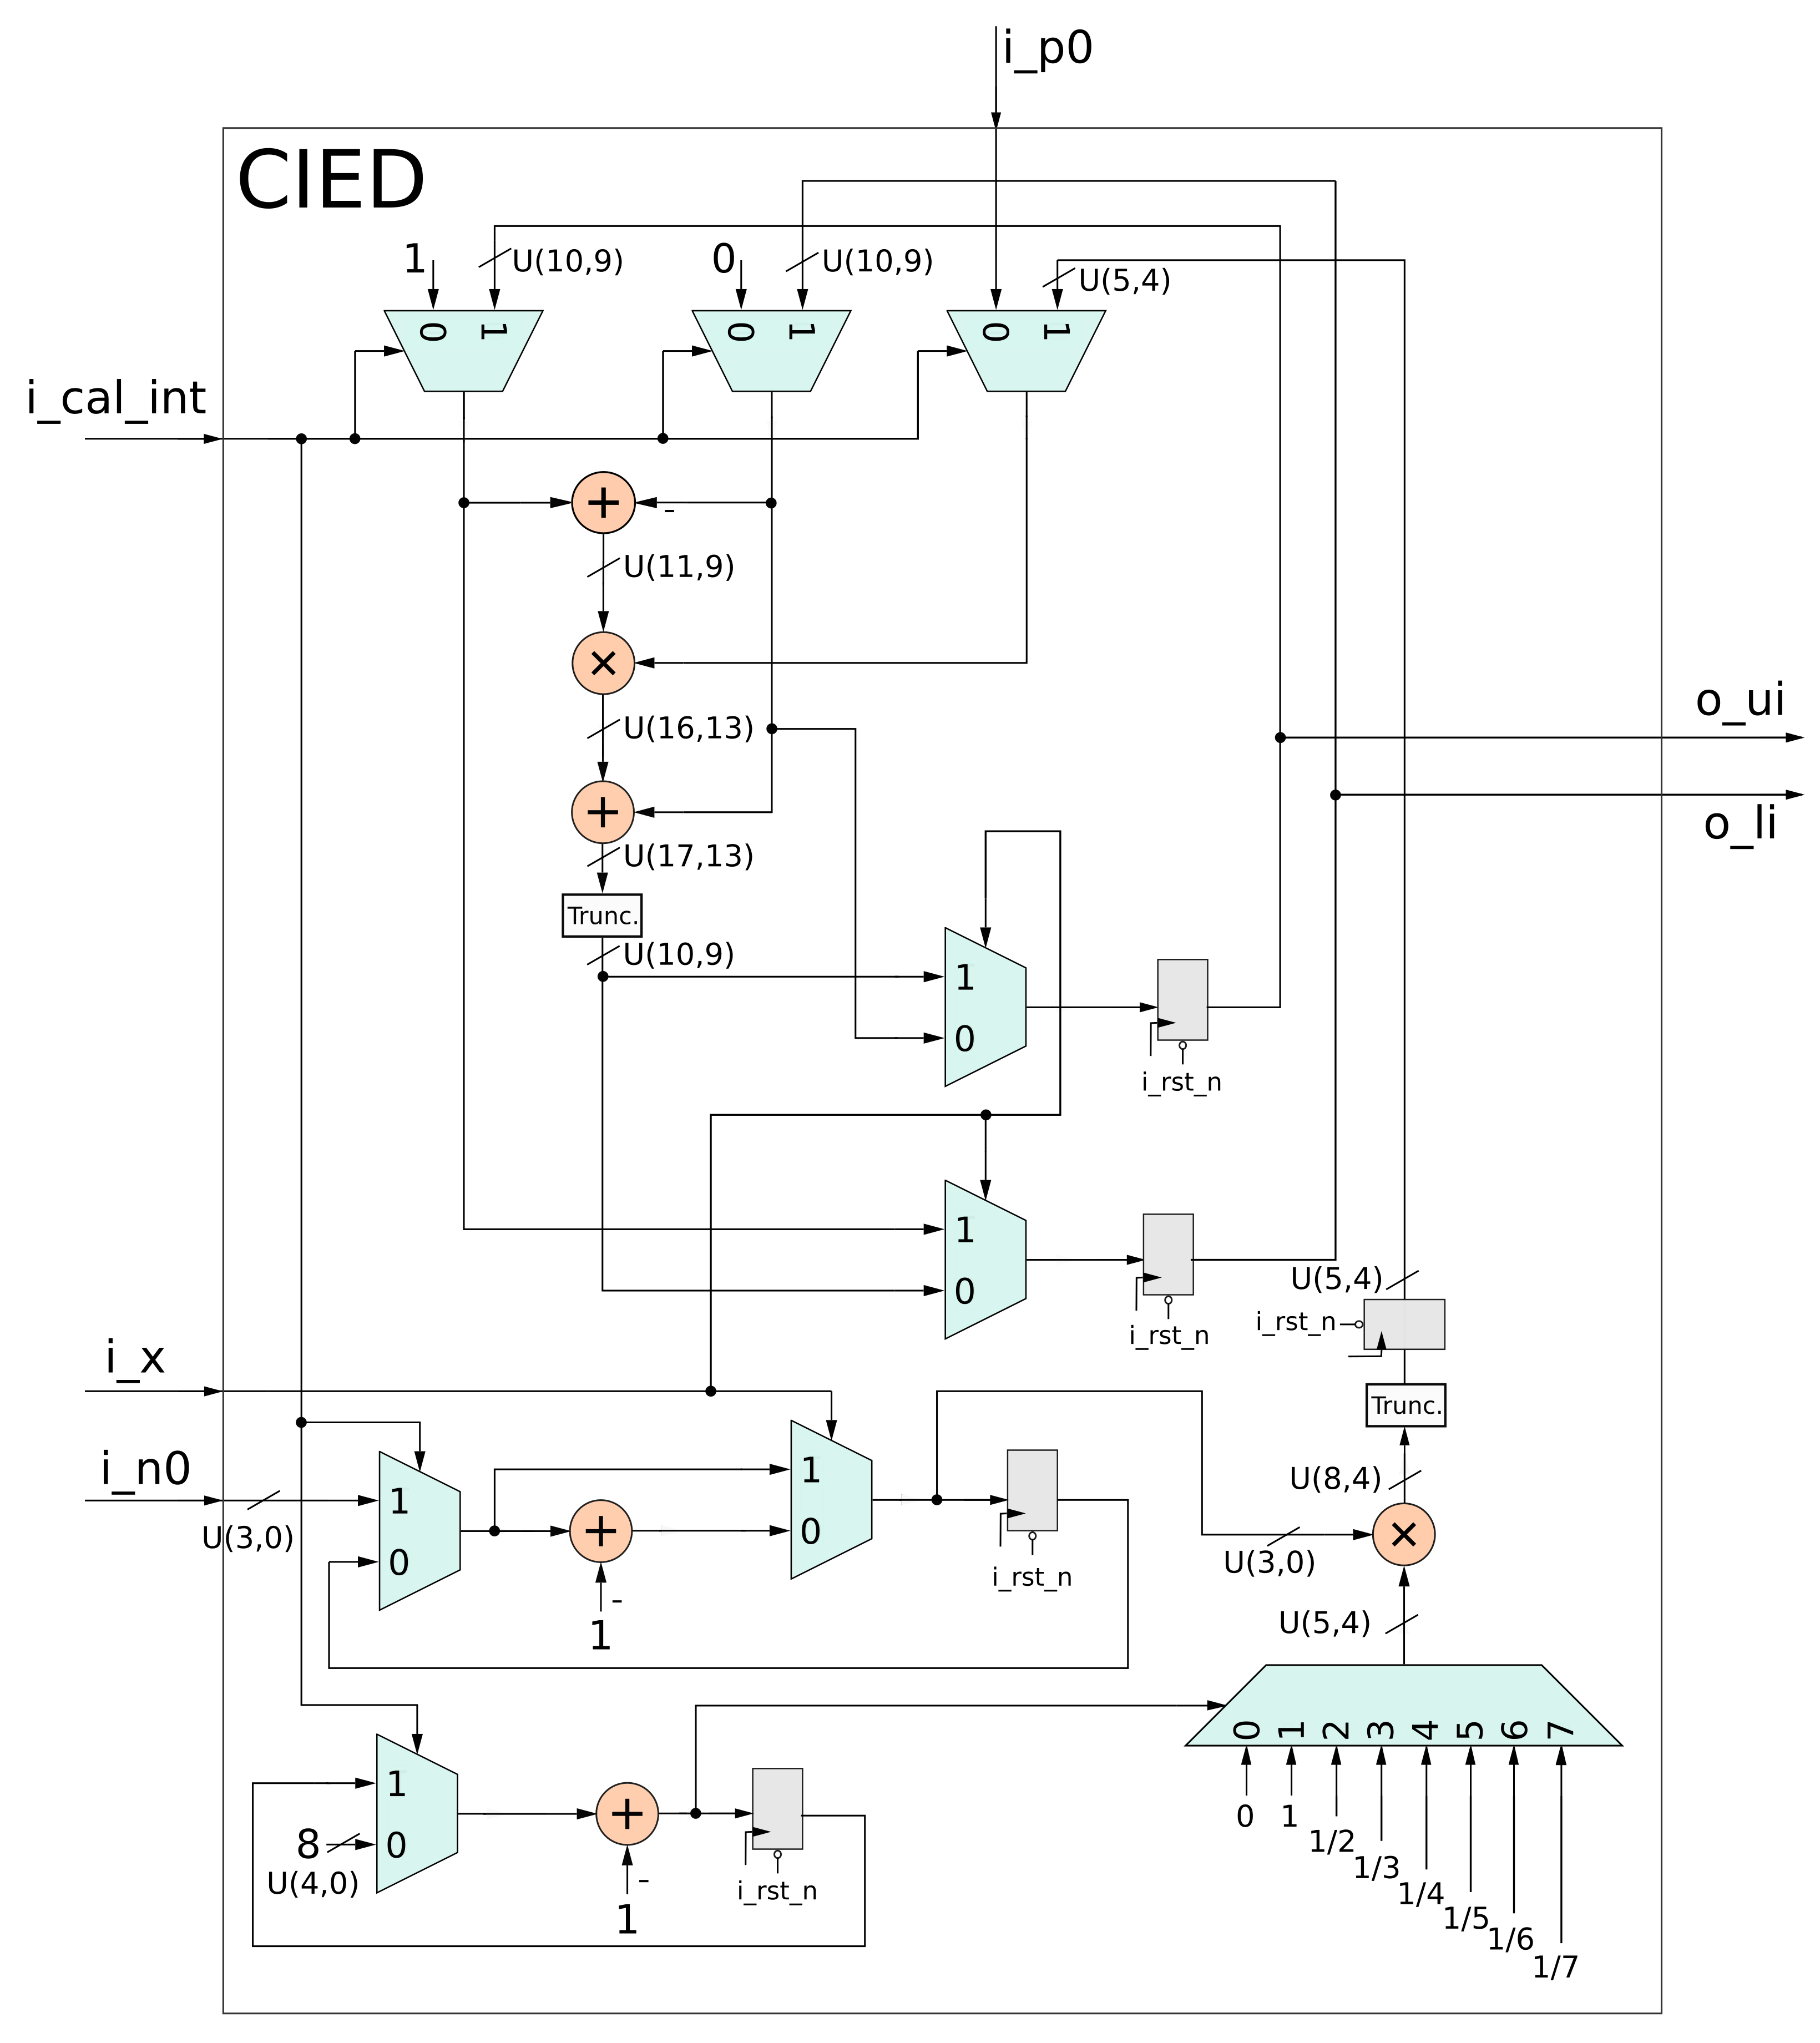
\includegraphics[height=0.85\paperheight]{Diagramas/internal_cied.png}%
\end{figure}
\end{frame}


\begin{frame}{Bloque CISD}

 \begin{figure}
  \centering
  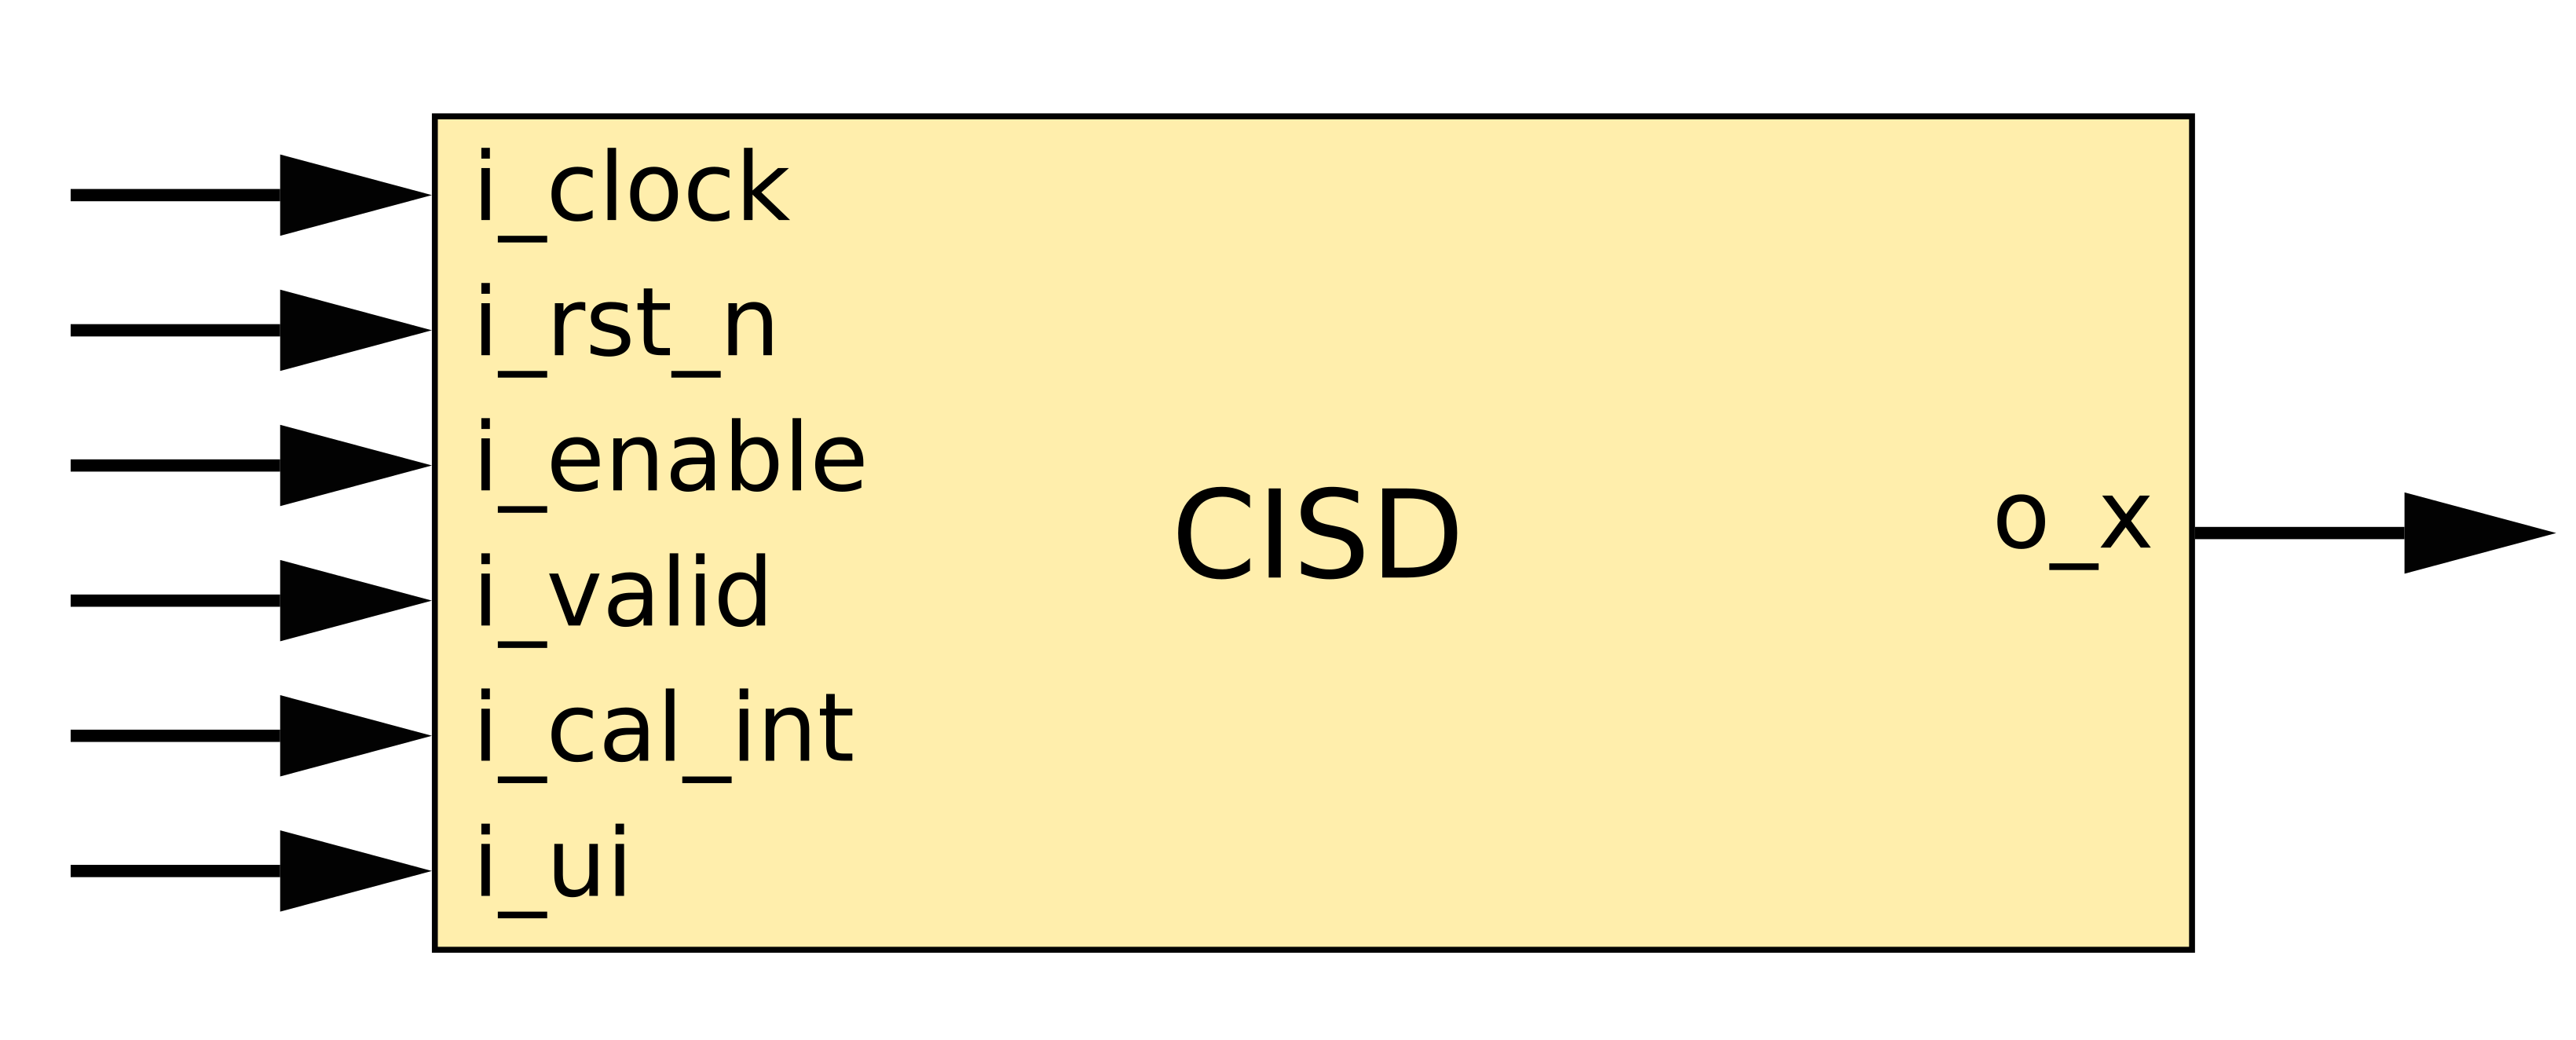
\includegraphics[width=0.70\paperwidth]{Diagramas/cisd.png}%
\end{figure}
\end{frame}

\begin{frame}{CISD, estructura interna}

 \begin{figure}
  \centering
  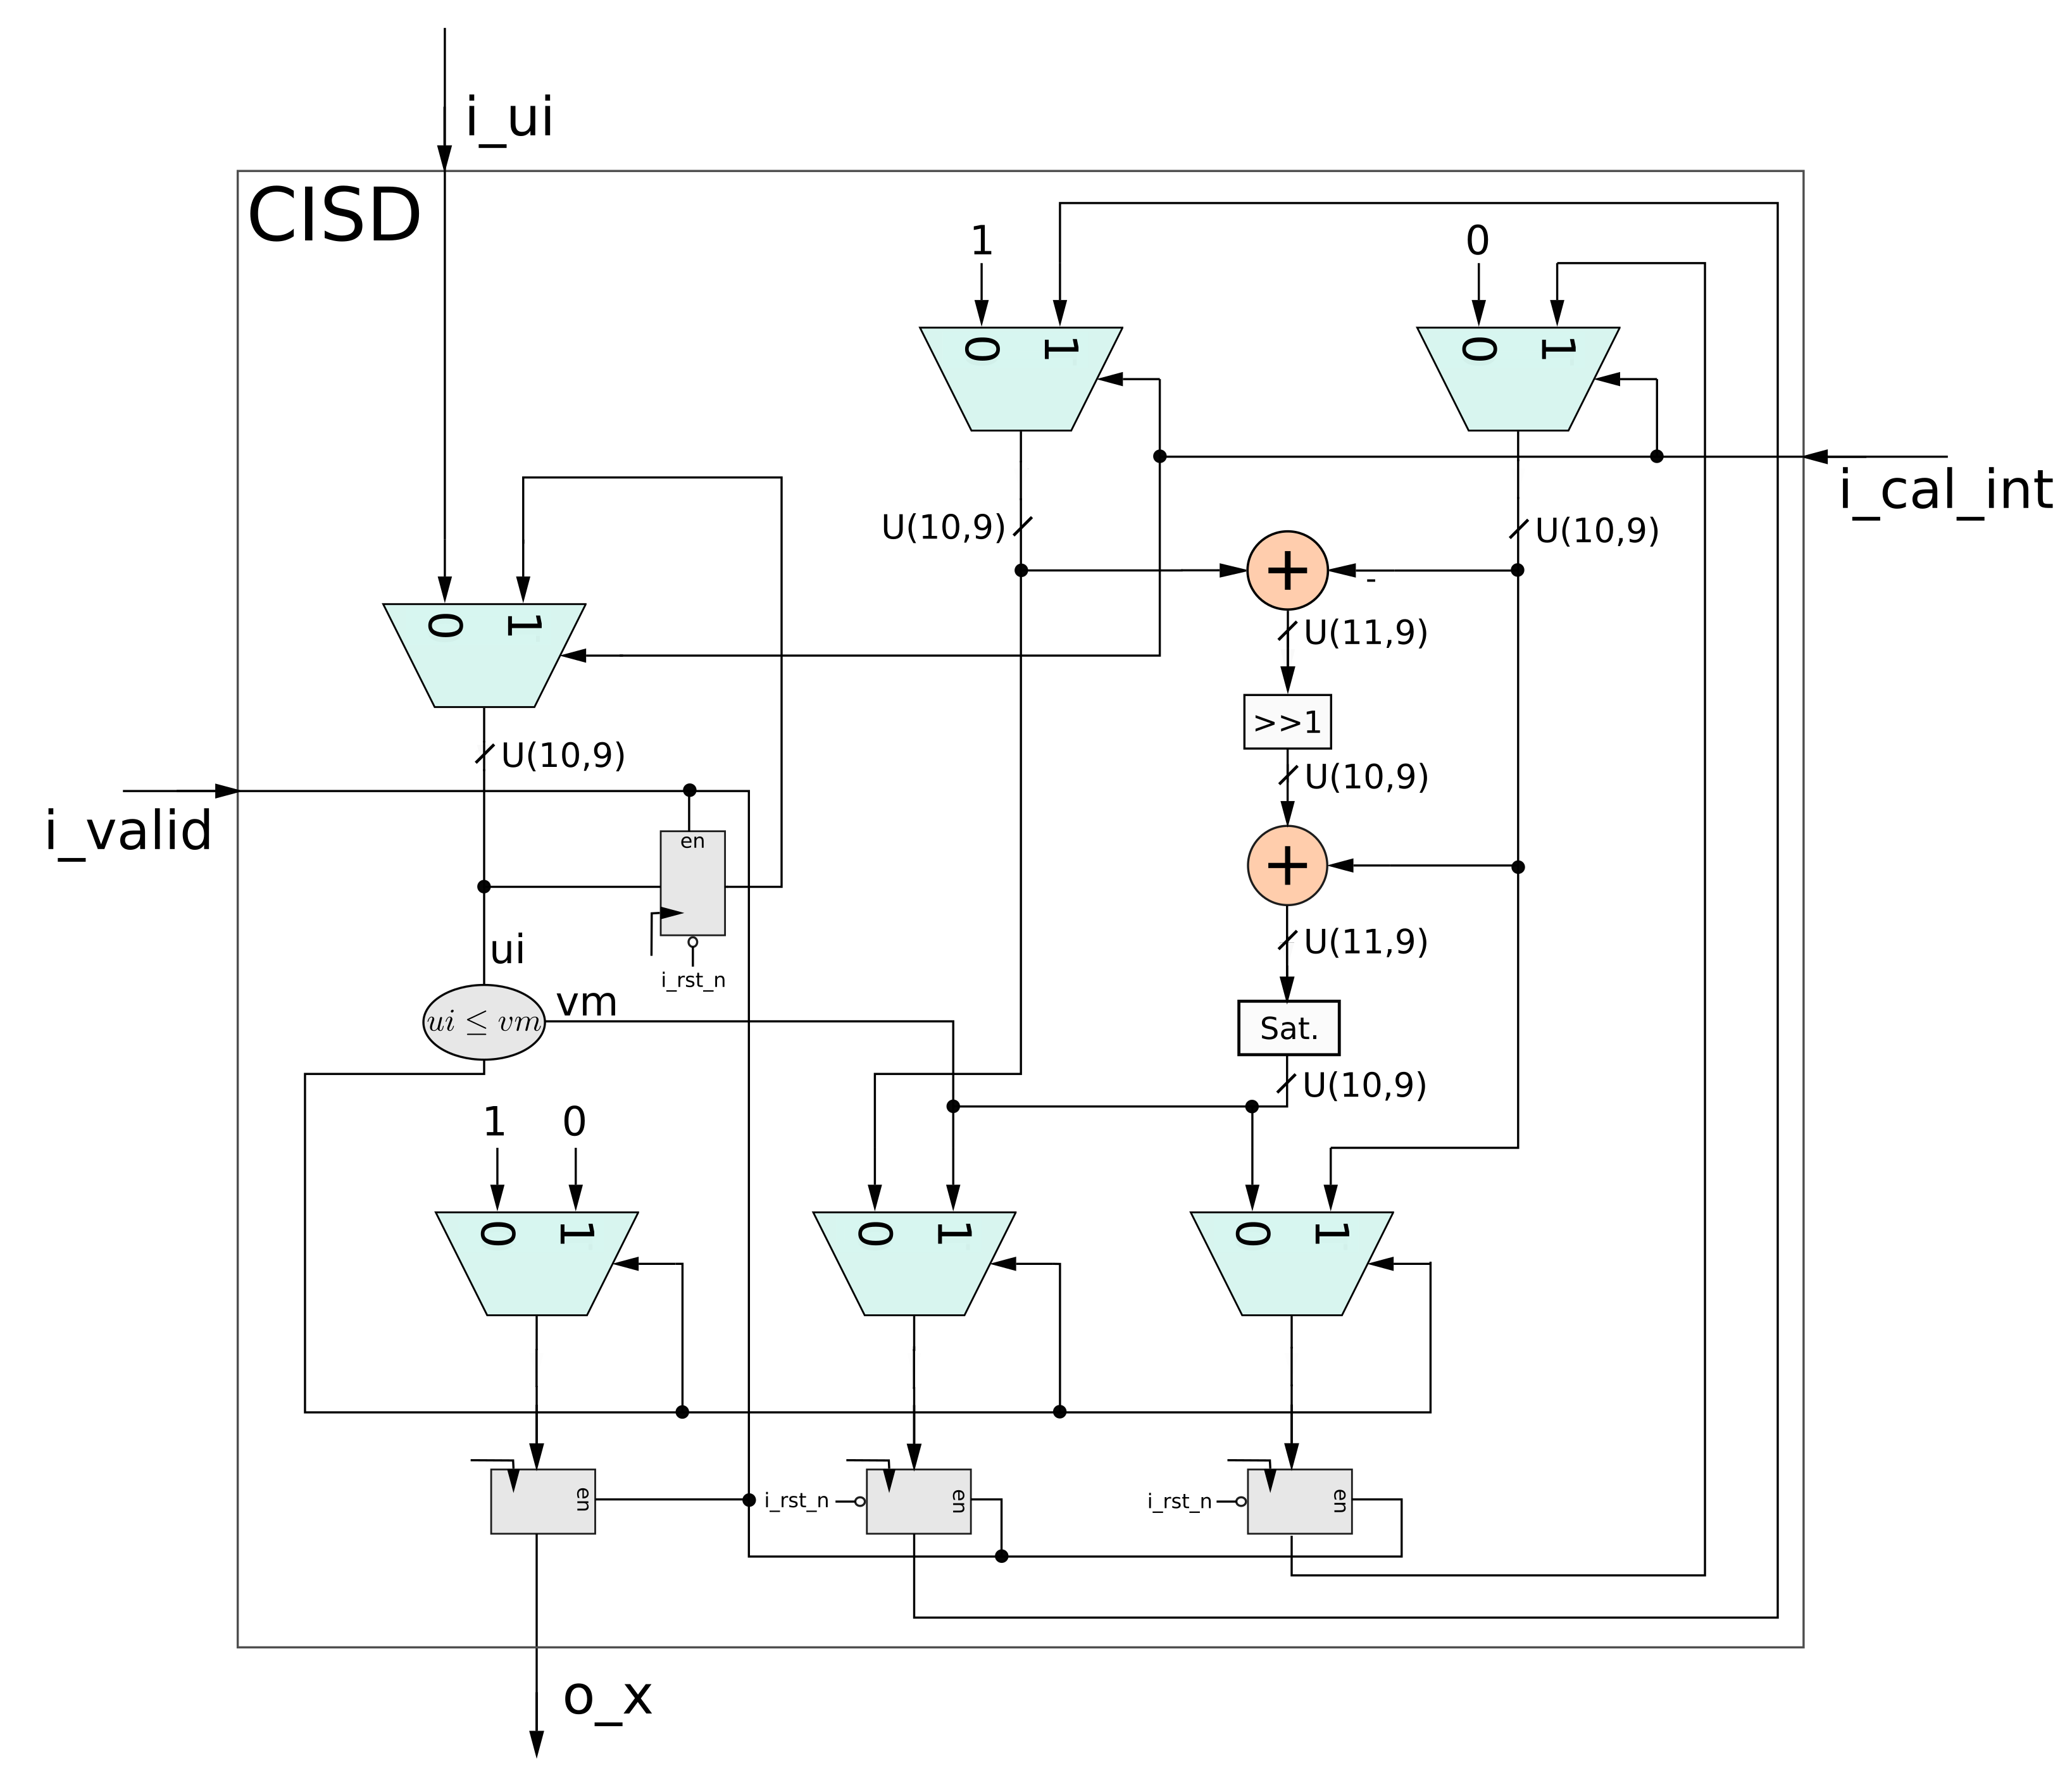
\includegraphics[width=0.70\paperwidth]{Diagramas/internal_cisd.png}%
\end{figure}
\end{frame}

\begin{frame}{Flujo de datos del decodificador}
    \begin{itemize}
        \item El bloque CISD requiere de 4 u.t. pero es habilitado por la FSM la mitad de los ciclos, por lo que requiere 8 u.t.
        \item Se ejecuta el bloque CISD cada ciclo, por lo que requiere 8 u.t.
        \item Esto implica que se generan 8 bits de salida cada 16 unidades de tiempo
    \end{itemize}
 \begin{figure}
  \centering
  \includegraphics[width=0.70\paperwidth]{Diagramas/grafo_dec.png}%
\end{figure}
\end{frame}

\begin{frame}{Dependencia de ejecuciones de codificador/decodificador}
    \begin{itemize}
        \item Para evitar un tiempo de procesamiento total de 16 u.t. se corren ambos procesos en paralelo
        \item Esto implica que se generan 8 bits de salida cada 8 u.t
    \end{itemize}
 \begin{figure}
  \centering
  \includegraphics[ height=0.60\paperheight]{Diagramas/dep_graph.png}%
\end{figure}
\end{frame}

\begin{frame}{Top FPGA}
 \begin{figure}
  \centering
  \includegraphics[ width=0.70\paperwidth]{Diagramas/fpga.png}%
\end{figure}
\end{frame}


\begin{frame}{Top FPGA, estructura interna }
 \begin{figure}
  \centering
  \includegraphics[ width=0.85\paperwidth]{Diagramas/internal_fpga.png}%
\end{figure}
\end{frame}


\begin{frame}{Bloque PAM-4}
\begin{itemize}
    \item El sistema implementa una modulación 16-QAM. Esta puede verse como dos canales PAM-4 (canal I y Q) 
\end{itemize}

 \begin{figure}
  \centering
  \includegraphics[ height=0.70\paperheight]{Diagramas/top_project.png}%
\end{figure}
\end{frame}

\begin{frame}{Bloque PRBS}
\begin{itemize}
    \item Para generar una modulación PAM-4 se utilizan dos PRBS. Una genera el bit de signo mientras y la otra el de magnitud. 
\end{itemize}

 \begin{figure}
  \centering
  \includegraphics[ width=0.70\paperwidth]{Diagramas/prbs.png}%
\end{figure}
\end{frame}


\begin{frame}{Bloque BER}
Consta de dos etapas:
\begin{enumerate}
    \item Sincroniza la secuencia de datos decodificada con la secuencia proveniente de la PRBS
    \item  Dos contadores de 64 bits almacenan la cantidad de muestras de entrada y de errores
\end{enumerate}
 \begin{figure}
  \centering
  \includegraphics[height=0.60\paperheight]{Diagramas/ber.png}%
\end{figure}
\end{frame}


\begin{frame}{Bloque GNG}
\begin{itemize}
    \item Permite medir nieveles de BER extremadamente bajos (~$10^{-15}$). El mismo fue obtenido de \cite{gng}. 
\end{itemize}


 \begin{figure}
  \centering
  \includegraphics[ width=0.70\paperwidth]{Diagramas/gng.png}%
\end{figure}
\end{frame}

\begin{frame}{GNG, estructura interna }
 \begin{figure}
  \centering
  \includegraphics[ width=0.85\paperwidth]{Diagramas/internal_gng.png}%
\end{figure}
\end{frame}

\subsection{Verificación}

\begin{frame}{Plataforma de verificación}
\begin{itemize}
    \item Permite controlar diferentes parámetros del sistema y obtener los datos del canal.
    \item Esta compuesto por:
    \begin{itemize}
        \item Programa de control
        \item Microcontrolador
        \item Register-file
        \item Memoria RAM
    \end{itemize}
\end{itemize}


\end{frame}



\begin{frame}{Comunicación serial}
\begin{itemize}
    \item Se utiliza un sistema de tramas largas y cortas 
\end{itemize}

\begin{figure}
  \centering
  \includegraphics[ height=0.70\paperheight]{Graficos/trama1.png}%
\end{figure}
\end{frame}

\begin{frame}{Comunicación GPIO}
\begin{itemize}
    \item Se utiliza para realizar la comunicación entre el microprocesador y el Register-file 
\end{itemize}
\begin{figure}
  \centering
  \includegraphics[ width=0.70\paperwidth]{Graficos/trama_GPIO.png}%
\end{figure}
\end{frame}

\begin{frame}{Implementación, resultados obtenidos}
\begin{itemize}
    \item Comparación entre implementación y modelo de punto flotante con codificador habilitado y deshabilitado.
\end{itemize}
\begin{figure}
  \centering
      \includegraphics[ width=0.75\paperwidth]{Graficos/BER_vs_SNR_fpga.png}%
\end{figure}
\end{frame}

\begin{frame}{Implementación, resultados obtenidos}
    \begin{itemize}
        \item Constelación del canal e histograma de símbolos para $P_{(s=1)}=0.75$
    \end{itemize}
    
\begin{columns}
    \begin{column}{0.48\paperwidth}
    \includegraphics[width=\textwidth]{Graficos/Channel_Constelation.png}%
    \end{column}
    \begin{column}{0.48\paperwidth}  
    \includegraphics[width=\textwidth]{Graficos/I_symbols_slicer.png}
    \end{column}
\end{columns}
\end{frame}

\begin{frame}{Implementación, resultados obtenidos}
     \begin{itemize}
        \item Constelación del canal e histograma de símbolos para $P_{(s=1)}=0.25$
    \end{itemize}
\begin{columns}
    \begin{column}{0.48\paperwidth}
    \includegraphics[width=\textwidth]{Graficos/Channel_Constelation_3.png}%
    \end{column}
    \begin{column}{0.48\paperwidth}  
    \includegraphics[width=\textwidth]{Graficos/I_symbols_slicer_3.png}
    \end{column}
\end{columns}
\end{frame}


\begin{frame}{Implementación, resultados obtenidos}
     \begin{itemize}
        \item Constelación del canal e histograma de símbolos para $P_{(s=1)}=0.5$
    \end{itemize}
\begin{columns}
    \begin{column}{0.48\paperwidth}
    \includegraphics[width=\textwidth]{Graficos/Channel_Constelation_2.png}%
    \end{column}
    \begin{column}{0.48\paperwidth}  
    \includegraphics[width=\textwidth]{Graficos/I_symbols_slicer_2.png}
    \end{column}
\end{columns}
\end{frame}

\section{Conclusiones}
\begin{frame}{Conclusiones}
    \begin{itemize}
    \item Técnica de `probabilistic shaping'
    \begin{itemize}
        \item Permite disminuir la tasa de error total del sistema
        \item Agrega una determinada cantidad de bits de redundancia
        \item Se vuelve mas eficiente a medida que la longitud de entrada aumenta 
    \end{itemize}
    \item Técnica de `constant distribution matching'
    \begin{itemize}
        \item Se debe utilizar técnica de escalado.
        \item La actualización de la nueva probabilidad implica realizar una división.
        \item Fácil adaptación a nuevas distribuciones de probabilidad. 
    \end{itemize}
    \item Implementación 
    \begin{itemize}
        \item El calculo de los intervalos, se puede realizar de manera recursiva o secuencial
        \item  El sistema implementado es poco practico para una longitud de entrada de 4 bits. 
    \end{itemize}
    \end{itemize}
\end{frame}

%
%

\section{Referencias}
\begin{frame}{Referencias}
        \bibliographystyle{unsrt}
        \bibliography{./biblio.bib}
\end{frame}

\end{document}